% !TeX program = pdflatex

\documentclass[manuscript,screen,review,natbib=false]{acmart}

% invited from LICS 2025 by the EIC

% \BibTeX command to typeset BibTeX logo in the docs
\AtBeginDocument{%
  \providecommand\BibTeX{{%
    Bib\TeX}}}

% !TEX root = main.tex

\newcommand\hmmax{0}
\newcommand\bmmax{0}
% \DeclareMathVersion{normal2}

% \usepackage{ebgaramond}
\ifluatex
% lualatex: acmart already loads fontspec/unicode-math and sets Linux Libertine O
% (TU encoding); the pdflatex font packages below would override that, and
% inputenc is a no-op, leaving \DeclareUnicodeCharacter undefined.
\else
\usepackage[T1]{fontenc}
\usepackage[utf8x]{inputenc}
\usepackage{type1ec}
\fi
% \usepackage{fontspec}
\usepackage{stmaryrd}
\usepackage{amsmath}
\usepackage{multicol}

% \usepackage{biblatex}
% \usepackage[natbib,style=authoryear,refsection=chapter]{biblatex}

\RequirePackage[datamodel=acmdatamodel, style=acmnumeric]{biblatex}

% \let\proof\relax
% \let\endproof\relax
\usepackage{amsthm}

% \usepackage{amssymb}
\usepackage{bbm}
\usepackage{dsfont}
\usepackage{mathtools}
\usepackage{thm-restate}
\usepackage{xspace}
\usepackage[textwidth=2cm,textsize=small]{todonotes}

\let\labelindent\relax
\usepackage{enumitem}
\usepackage{hyperref}
\usepackage{cleveref}
\usepackage{stackrel}
% \usepackage{MnSymbol} % for \cupdot
\usepackage{todonotes}
% \usepackage{shuffle}
% \usepackage{paralist}
\usepackage{graphicx}
\usepackage{etoolbox}
\usepackage{textcase}
\usepackage[bb=boondox]{mathalfa}
\usepackage{verbatim}

\usepackage[contents={}]{background}
% \newcommand\BGfrom[1]{%
% \AddEverypageHook{%
%   \ifnum\value{page}>\numexpr#1-1\relax
%     \backgroundsetup{
%       contents={Over the limit},
%       color=red,
%       scale=10,
%       opacity=0.5
%     }%
%   \fi
%   \BgMaterial%
%   }%
% }
% adds a red background for pages after the limit
% \BGfrom{7}

\usepackage{amstext} % for \text macro
\usepackage{array}   % for \newcolumntype macro
\newcolumntype{C}{>{$}c<{$}} % math-mode version of "c" column type
\newcolumntype{L}{>{$}l<{$}} % math-mode version of "l" column type

\hypersetup{
    colorlinks,
    linkcolor={red!50!black},
    citecolor={blue!50!black},
    urlcolor={blue!80!black}
}

\usepackage{tikz}
\usetikzlibrary{positioning}
\usetikzlibrary{decorations.markings}

\makeatletter
\patchcmd{\@sect}{\uppercase}{\MakeTextUppercase}{}{}
\patchcmd{\@sect}{\uppercase}{\MakeTextUppercase}{}{}
\makeatother
%!TEX root main.tex

% general macros
\newcommand{\tuple}[1]{(#1)}
\newcommand{\tuplesmall}[1]{(#1)}
\newcommand{\goesto}[1]{\xrightarrow{#1}}
\newcommand{\from}{\leftarrow}
\newcommand{\e}{\varepsilon}
\newcommand{\sep}{\mid}

\newcommand{\ignore}[1]{}

% English
\newcommand{\wlg}{w.l.o.g.}
\newcommand{\Wlg}{W.l.o.g.}
\newcommand{\wrt}{w.r.t.}
\newcommand{\vs}{vs.}
\newcommand{\cf}{cf.}
\newcommand{\eg}{e.g.}
\newcommand{\Eg}{E.g.}
\newcommand{\aka}{a.k.a.}
\newcommand{\ie}{i.e.}
\newcommand{\Ie}{I.e.}
\newcommand{\rhs}{r.h.s.}
\newcommand{\lhs}{l.h.s.}
\newcommand{\egs}{EGS}
\newcommand{\etal}{\emph{et al.}}
\newif\ifstartedinmathmode
\newcommand*{\st}{%s.t.~
  \relax\ifmmode\startedinmathmodetrue\else\startedinmathmodefalse\fi
  \ifstartedinmathmode{\;\cdot\;}\else{s.t.}\fi%
}

\makeatletter
\providecommand*{\cupdot}{%
  \mathbin{%
    \mathpalette\@cupdot{}%
  }%
}
\newcommand*{\@cupdot}[2]{%
  \ooalign{%
    $\m@th#1\cup$\cr
    \hidewidth$\m@th#1\cdot$\hidewidth
  }%
}
\makeatother

% sets
\newcommand{\A}{\mathbb A}
\renewcommand{\AA}{\mathcal A}
\newcommand{\B}{\mathbb B}
\newcommand{\BB}{\mathcal B}
\newcommand{\C}{\mathbb C}
\newcommand{\D}{\mathbb D}
\newcommand{\F}{\mathbb F}
\renewcommand{\H}{\mathbb H}
\newcommand{\N}{\mathbb N}
\newcommand{\Z}{\mathbb Z}
\newcommand{\Q}{\mathbb Q}
\newcommand{\R}{\mathbb R}
\renewcommand{\S}{\mathbb S}
\newcommand{\Sleft}{\S^{\mathsf L}}
\newcommand{\Sright}{\S^{\mathsf R}}
\newcommand{\Ssyn}{\S_{\text{syn}}}
\renewcommand{\SS}{\mathcal S}
\newcommand{\T}{\mathbb T}
\newcommand{\Tleft}{\T^{\mathsf L}}
\newcommand{\Tright}{\T^{\mathsf R}}
\newcommand{\Tsyn}{\T_{\text{syn}}}
\newcommand{\TT}{\mathcal T}
\newcommand{\V}{\mathbb V}
\renewcommand{\k}{\kappa}
\renewcommand{\a}{\mathfrak a}

\newcommand{\x}{\mathtt x}
\newcommand{\y}{\mathtt y}
\newcommand{\z}{\mathtt z}

\newcommand{\FF}{\mathcal F}
\newcommand{\GG}{\mathcal G}

% maths
\let\oldcirc\circ
\let\circ\relax
\DeclareMathOperator{\circ}{\oldcirc\,}

\newcommand{\compose}[1]{\,\oldcirc_{#1}\,}

\DeclareMathOperator{\binconv}{\ast}
% \DeclareMathOperator{\rel}{{\ensuremath R}}
\DeclareMathOperator{\bisimulation}{\sim}

\newcommand{\rel}{\mathrel R}
\newcommand{\relation}[1]{\mathrel {#1}}
\newcommand{\tilderel}{\mathrel {\widetilde R}}
\newcommand{\tilderelation}[1]{\mathrel {\widetilde {#1}}}

% METAFONT mumbo-jumbo for shuffle
% \DeclareSymbolFont{Shuffle}{U}{shuffle}{m}{n}
% \DeclareFontFamily{U}{shuffle}{}
% \DeclareFontShape{U}{shuffle}{m}{n}{%
%   <-8>shuffle7%
%   <8->shuffle10%
% }{}
% \DeclareMathSymbol\shuffle{\mathbin}{Shuffle}{"001}
% \DeclareMathSymbol\cshuffle{\mathbin}{Shuffle}{"002}

% \let\oldshuffle\shuffle
% \let\shuffle\relax
% \DeclareMathOperator{\shuffle}{\oldshuffle}
% \newcommand{\shufflepower}[2]{{#1}^{\oldshuffle#2}}
% \newcommand{\shinv}[1]{\shufflepower {#1}{-1}}

% shuffle by hand
% https://tex.stackexchange.com/questions/183988/how-to-make-the-shuffle-product-symbol-in-latex-math-mode
\makeatletter
\providecommand*{\shuffle}{%
  \mathbin{\mathpalette\shuffle@{}}%
}
\newcommand*{\shuffle@}[2]{%
  % #1: math style
  % #2: unused
  \sbox0{$#1\vcenter{}$}%
  \kern .15\ht0 % side bearing
  \rlap{\vrule height .25\ht0 depth 0pt width 2.5\ht0}%
  \raise.1\ht0\hbox to 2.5\ht0{%
    \vrule height 1.75\ht0 depth -.1\ht0 width .17\ht0 %
    \hfill
    \vrule height 1.75\ht0 depth -.1\ht0 width .17\ht0 %
    \hfill
    \vrule height 1.75\ht0 depth -.1\ht0 width .17\ht0 %
  }%
  \kern .15\ht0 % side bearing
}
\makeatother

\let\oldcolon\colon
\let\colon\relax
\DeclareMathOperator{\colon}{\,:\,}

\let\oldmod\mod
\let\mod\relax
\DeclareMathOperator{\mod}{mod}

\DeclareMathOperator{\cauchy}{\ast}
\DeclareMathOperator{\hadamard}{\odot}
\DeclareMathOperator{\infiltration}{\uparrow}
\DeclareMathOperator{\product}{\ast}
% \DeclareMathOperator{\sq}{\Box}%{\circ_\C}
% \DeclareMathOperator{\binconv}{\ast}
\newcommand{\norm}[2]{\left| #2 \right|_{#1}}
\newcommand{\onenorm}[1]{\norm 1 {#1}}
\newcommand{\inftynorm}[1]{\norm \infty {#1}}
\newcommand{\height}[1]{\inftynorm{#1}}
\newcommand{\limplies}{\Rightarrow}
\newcommand{\valname}{v}
\newcommand{\val}[1]{\valname({#1})}
\newcommand{\valpname}[1]{\valname_{#1}}
\newcommand{\valp}[2]{\valpname {#1}({#2})}
\newcommand{\valstar}[1]{\valname^*({#1})}
\newcommand{\eval}[2]{\left.#1\right|_{#2}}
\newcommand{\floor}[1]{\lfloor#1\rfloor}
\newcommand{\abs}[1]{\left|#1\right|}
\newcommand{\card}[1]{\left|#1\right|}
\newcommand{\length}[2]{\left|#2\right|_{#1}}
\newcommand{\len}[1]{\left|#1\right|}
\newcommand{\set}[1]{\left\{#1\right\}}
\newcommand{\setof}[2]{\set{#1 \;\middle|\; #2}}
\newcommand{\multiset}[1]{\left\{\!\left\{#1\right\}\!\right\}}
\newcommand{\multisetof}[2]{\multiset{#1 \mid #2}}
\newcommand{\census}[1]{\mathsf{c}\left(#1\right)}
\newcommand{\eqclass}[2]{\left[#2\right]_{#1}}
% \newcommand{\averagefun}{\mathsf{avg}}
% \newcommand{\average}[2]{\averagefun_{#1}\left(#2\right)}
\newcommand{\average}[2]{\left\{#2\right\}_{#1}}
\newcommand{\commclass}[1]{\widetilde {#1}}
\newcommand{\rad}[1]{\sqrt{#1}}
\newcommand{\polyexpr}[2]{#1\{#2\}}
\newcommand{\poly}[2]{#1[#2]}
\newcommand{\polyof}[3]{\poly {#1} {#2 \mid #3}}
\newcommand{\diffpoly}[2]{\poly{#1}{#2}^{(*)}}
\newcommand{\ncpoly}[2]{#1\langle#2\rangle}
\newcommand{\rational}[2]{#1(#2)}
\newcommand{\Lie}[2]{\mathsf{Lie}_{#1}\langle#2\rangle}
\newcommand{\LieDeg}[3]{\mathsf{Lie}^{#1}_{#2}\langle#3\rangle}
\newcommand{\rat}[2]{#1(#2)}
\newcommand{\lparenangle}{{\,\mathclap{(}\!\langle}}
\newcommand{\rparenangle}{{\,\mathclap{\rangle}\!)}}
\newcommand{\ncrat}[2]{#1\lparenangle#2\rparenangle}
\newcommand{\nclaurent}[2]{#1\lparenangle\!\lparenangle#2\rparenangle\!\rparenangle}
\newcommand{\powerseries}[2]{#1[\![#2]\!]}
\newcommand{\algps}[2]{\powerseries {#1} {#2}_{\mathsf{alg}}}
\newcommand{\laurentseries}[2]{#1(\!(#2)\!)}
\newcommand{\series}[2]{#1\langle\!\langle#2\rangle\!\rangle}
\newcommand{\lcseries}[2]{#1\langle\!\langle#2\rangle\!\rangle^{\text{LC}}}
\newcommand{\commseries}[2]{#1\langle\!\langle#2\rangle\!\rangle^{\mathsf{comm}}}
\newcommand{\algseries}[2]{#1\langle\!\langle#2\rangle\!\rangle_{\mathsf{alg}}}
\newcommand{\sequences}[2]{#1[\![\N^{#2}]\!]}
\newcommand{\matrices}[3]{#3^{#1 \times #2}}
% \newcommand{\lin}[2]{\langle #2 \rangle_{#1}}
% \newcommand{\linof}[3]{\lin {#1} {#2 \mid #3}}
\newcommand{\ideal}[1]{\langle#1\rangle}
\newcommand{\idealof}[2]{\ideal{#1 \mid #2}}
\newcommand{\diffideal}[1]{\ideal{#1}^{(*)}}
\newcommand{\diffidealof}[2]{\idealof{#1}{#2}^{(*)}}
\newcommand{\module}[1]{\langle#1\rangle}
\newcommand{\moduleof}[2]{\module{#1 \mid #2}}
\newcommand{\lin}[2]{\mathsf{Lin}_{#2}\left(#1\right)}
% \newcommand{\linof}[3]{\lin{#1 \mid #2} {#3}}
\renewcommand{\dim}[1]{\mathsf{dim}\,{#1}}
\newcommand{\leadingterm}[1]{\mathsf{lt}\,{#1}}
\newcommand{\sem}[1]{\llbracket#1\rrbracket}
\newcommand{\Asem}[2]{#1\sem{#2}}
\newcommand{\support}[1]{\mathsf{supp}(#1)}
% \newcommand{\lang}[1]{L\left(#1\right)}
\newcommand{\bigO}[1]{O\left(#1\right)}
\newcommand{\bigOmega}[1]{\Omega\left(#1\right)}
\newcommand{\multiplicity}[2]{\#({#2})_{#1}}
\newcommand{\Parikh}[1]{\mathrm c({#1})}
\newcommand{\Parikhinv}[1]{\mathrm c^{-1}({#1})}
\newcommand{\coefficient}[2]{[#1]#2}
\newcommand{\restrict}[2]{\left.#1\right|_{#2}}
\newcommand{\restrictsmall}[2]{#1|_{#2}}
\newcommand{\equivmod}[3]{{#1} \equiv {#2}\; (\mathsf{mod}\ #3)}
\newcommand{\ord}[1]{\mathsf{ord}(#1)}
\newcommand{\comm}[2]{\mathsf{comm}_{#1}(#2)}
\newcommand{\stops}[1]{\mathsf{s2p}\left(#1\right)}
\newcommand{\pstos}[1]{\mathsf{p2s}\left(#1\right)}
\newcommand{\iso}{\cong}
\newcommand{\completion}[1]{\widehat{#1}}
\newcommand{\linearspan}[2]{\mathsf{Lin}_{#1}(#2)} %{\langle#1\rangle}
\newcommand{\inner}[2]{\langle#1, #2\rangle}
\newcommand{\closure}[1]{\overline{#1}}
\newcommand{\reversal}[1]{{#1}^\mathsf{rev}}
\newcommand{\transpose}[1]{{#1}^\mathsf{T}}
\newcommand{\id}{\mathsf{id}}
%\newcommand{\leftright}[3]{{#2}^{#1, #3}}
\newcommand{\leftright}[3]{\mbox{}^{#1}{#2}^{#3}}
\newcommand{\lr}[3]{\leftright{#1}{#2}{#3}}
\renewcommand{\iff}{\Leftrightarrow}

\newcommand{\seq}[2]{\left(#1 \mapsto {#2}\right)}
\newcommand{\derive}[1]{\delta_{#1}}
\newcommand{\deriveleft}[1]{\delta^L_{#1}}
\newcommand{\deriveright}[1]{\delta^R_{#1}}
\DeclareRobustCommand{\atled}{\text{\reflectbox{$\delta$}}}
\newcommand{\derleft}[2]{{#1}^{-1} {#2}}
\newcommand{\derright}[2]{{#2} {#1}^{-1}}
\newcommand{\class}[2]{[#1]_{#2}}
\let\oldpartial\partial
% \renewcommand{\partial}[2]{\frac {\oldpartial {#2}} {\oldpartial {#1}}}
\renewcommand{\partial}[2]{\oldpartial_{#1}{#2}}
\newcommand{\partialk}[3]{\oldpartial_{#1}^{#2}{#3}}
\newcommand{\bigpartial}[2]{\frac {\oldpartial {#2}} {\oldpartial{#1}}}
\newcommand{\dn}[2]{\mathrm d^{#1} {#2}}
\renewcommand{\d}[1]{\dn {} {#1}}
\newcommand{\total}[2]{\frac {\d {#1}}{\d {#2}}}
\newcommand{\totaln}[3]{\frac {\dn {#1} {#2}}{\d {#3}^{#1}}}
\newcommand{\jacobian}[2]{\partial{#1}{#2}}
\newcommand{\shift}[1]{\sigma_{#1}}
\newcommand{\deductionrule}[2]{\begin{array}{c}%
{#1} \\ \hline {#2}%
\end{array}}
\newcommand{\one}{\mathbbm 1}
\newcommand{\zero}{\mathbb 0}

\newcommand{\X}{\mathcal X}
\newcommand{\Y}{\mathcal Y}
\newcommand{\ZZ}{\mathcal Z}
\newcommand{\ZERO}{\mathbf 0}
\newcommand{\ONE}{\mathbf 1}
\newcommand{\EGS}[1]{\mathsf{EGS}[#1]}
\newcommand{\SETSP}{\mathsf{SET}}
\newcommand{\SET}[1]{\SETSP[#1]}
\newcommand{\SEQSP}{\mathsf{SEQ}}
\newcommand{\SEQ}[1]{\SEQSP[#1]}
\newcommand{\CYCSP}{\mathsf{CYC}}
\newcommand{\CYC}[1]{\CYCSP[#1]}
\newcommand{\TREE}[2]{\mathsf{T}_{#2}[#1]}
\newcommand{\CATALAN}[1]{\mathsf{T}[#1]}
\newcommand{\CAYLEY}[1]{\mathsf{C}[#1]}
\newcommand{\SPGRAPHS}[1]{\mathsf{SP}[#1]}
\newcommand{\SGRAPHS}[1]{\mathsf{S}[#1]}
\newcommand{\PGRAPHS}[1]{\mathsf{P}[#1]}

\newcommand{\lneg}{\neg}
\newcommand{\erf}{\mathrm{erf}}
\newcommand{\arsinh}{\mathrm{arsinh}}
\newcommand{\arcosh}{\mathrm{arcosh}}
\newcommand{\artanh}{\mathrm{artanh}}
\newcommand{\csch}{\mathrm{csch}}
\newcommand{\sech}{\mathrm{sech}}

% acronyms
\newcommand{\CDF}{\textsf{CDF}}
\newcommand{\CDA}{\textsf{CDA}}
\newcommand{\BPP}{\textsf{BPP}}
\newcommand{\WBPP}{\textsf{WBPP}}
\newcommand{\WFA}{\textsf{WFA}}
\newcommand{\WTS}{\textsf{WTS}}
\newcommand{\LTS}{\textsf{LTS}}
\newcommand{\ATS}{\textsf{ATS}}

\newcommand{\NC}{\textsf{NC}}
\newcommand{\coRNC}{\textsf{coRNC}}
\newcommand{\PTIME}{\textsf{PTIME}}
\newcommand{\coRP}{\textsf{coRP}}
\newcommand{\PSPACE}{\textsf{PSPACE}}
\newcommand{\EXPTIME}{\textsf{EXPTIME}}
\newcommand{\NEXPTIME}{\textsf{NEXPTIME}}
\newcommand{\coNEXPTIME}{\textsf{coNEXPTIME}}
\newcommand{\EXPSPACE}{\textsf{EXPSPACE}}
\newcommand{\TWOEXPTIME}{{2-\EXPTIME}}
\newcommand{\TWONEXPTIME}{{2-\NEXPTIME}}
\newcommand{\coTWONEXPTIME}{{2-\coNEXPTIME}}
\newcommand{\TWOEXPSPACE}{{2-\EXPSPACE}}

\newcolumntype{A}{
 >{$}r<{$}
 @{\extracolsep{0pt}}
 >{${}} l <{$}
% @{\extracolsep{\fill}}
} % A for "align"
%% (1) "r" column in math mode:          >{$} r <{$}
%% (2) no space:                         @{}
%% (3) "l" column in math mode, with
%%     an empty subformula at the start: >{${}} l <{$}

\newcolumntype{M}{
 >{$}c<{$}
}

% theorems
\theoremstyle{plain}
\newtheorem{theorem}{Theorem}
\newtheorem*{theorem*}{Theorem}
\newtheorem{lemma}[theorem]{Lemma}
\newtheorem{corollary}[theorem]{Corollary}
\newtheorem{claim}[theorem]{Claim}
\newtheorem*{claim*}{Claim}
\newtheorem{proposition}[theorem]{Proposition}
\newtheorem*{proposition*}{Proposition}
\newtheorem{fact}[theorem]{Fact}
\newtheorem*{fact*}{Fact}

\theoremstyle{remark}
\newtheorem{remark}{Remark}
\newtheorem{example}{Example}

\theoremstyle{definition}
\newtheorem{definition}{Definition}

\theoremstyle{problem}
\newtheorem{problem}{Problem}

\let\oldproof\proof
\let\endoldproof\endproof

% \makeatletter
% \let\proof\@undefined
% \let\endproof\@undefined 
% \makeatother
% \newenvironment{proof}{\oldproof}{\endoldproof}

% \newenvironment{myproof}{\comment}{\endcomment}
\newenvironment{myproof}{\proof}{\endproof}

\newenvironment{claimproof}{\begin{proof}[Proof of the claim]}{\end{proof}}

% \newenvironment{myclaimproof}{\comment}{\endcomment}
\newenvironment{myclaimproof}{\begin{claimproof}}{\end{claimproof}}

\crefname{equation}{}{}%{Eq.}{Eqns.}
\crefname{definition}{Definition}{Definitions}
\crefname{claim}{Claim}{Claims}
\crefname{proposition}{Proposition}{Propositions}
\crefname{lemma}{Lemma}{Lemmas}
\crefname{corollary}{Corollary}{Corollaries}
\crefname{theorem}{Theorem}{Theorems}
\crefname{figure}{Fig.}{Figures}
\crefname{fact}{Fact}{Facts}
\crefname{example}{Example}{Examples}
\crefname{remark}{Remark}{Remarks}
\crefname{section}{§}{§§}
\crefname{subsection}{§}{§§}
\crefname{subsubsection}{§}{§§}
\crefname{enumi}{}{}
\crefname{problem}{Problem}{Problems}

\crefname{table}{Table}{Tables}
\crefname{figure}{Figure}{Figures}

\crefname{appendix}{Appendix}{Appendices}

% TODO
\newcommand{\ilorenzo}[1]{\todo[inline, color=blue!30]{\textsf L: #1}}
\newcommand{\lorenzo}[1]{\todo[color=blue!30]{\textsf L: #1}}

% for making Nguy\~{\^{e}}n work with biber..v.
% (pdflatex only; under lualatex Linux Libertine O has the glyph natively)
\ifdefined\DeclareUnicodeCharacter\DeclareUnicodeCharacter{1EC5}{\~{\^{e}}}\fi

\addbibresource{master.bib} 
\addbibresource{books.bib}
\addbibresource{extra.bib}

%% Rights management information.  This information is sent to you
%% when you complete the rights form.  These commands have SAMPLE
%% values in them; it is your responsibility as an author to replace
%% the commands and values with those provided to you when you
%% complete the rights form.
\setcopyright{cc}% acmlicensed
\copyrightyear{2025}
\acmYear{2025}
\acmDOI{XXXXXXX.XXXXXXX}
%% These commands are for a PROCEEDINGS abstract or paper.
% \acmConference[Conference acronym 'XX]{Make sure to enter the correct
%   conference title from your rights confirmation email}{June 03--05,
%   2018}{Woodstock, NY}
%%
%%  Uncomment \acmBooktitle if the title of the proceedings is different
%%  from ``Proceedings of ...''!
%%
%%\acmBooktitle{Woodstock '18: ACM Symposium on Neural Gaze Detection,
%%  June 03--05, 2018, Woodstock, NY}
% \acmISBN{978-1-4503-XXXX-X/2018/06}

% \acmJournal{JACM}

%%
%% Submission ID.
%% Use this when submitting an article to a sponsored event. You'll
%% receive a unique submission ID from the organizers
%% of the event, and this ID should be used as the parameter to this command.
%%\acmSubmissionID{123-A56-BU3}

% \citestyle{acmauthoryear}

\begin{document}

\title
  [The commutativity problem for effective varieties of formal series]
  {The commutativity problem for effective varieties of formal series,\\ and applications}

\author{Lorenzo Clemente}
\authornote{We acknowledge partial support of the NCN Sonata Bis grant 2024/54/E/ST6/00287
and of the ERC Starting grant INFSYS, agreement no. 950398.}
\email{clementelorenzo@gmail.com}
\orcid{0000-0003-0578-9103}
\affiliation{%
  \institution{Dept.~of Mathematics, Informatics and Mechanics, University of Warsaw}
  \city{Warszawa}
  % \state{}
  \country{Poland}
}

% \renewcommand{\shortauthors}{Clemente}

\begin{abstract}
  A \emph{formal series} in noncommuting variables $\Sigma$ over the rationals is a mapping $\Sigma^* \to \Q$
  from the free monoid generated by $\Sigma$ to the rationals.
  %
  We say that a series is \emph{commutative} if the value in the output
  does not depend on the order of the symbols in the input.
  %
  The \emph{commutativity problem} for a class of series
  takes as input a (finite presentation of) a series from the class
  and amounts to establishing whether it is commutative.
  %
  This is a very natural, albeit nontrivial problem,
  which has not been considered before from an algorithmic perspective.

  We show that commutativity is decidable
  for all classes of series that constitute a so-called \emph{effective prevariety},
  a notion generalising Reutenauer's varieties of formal series.
  %
  For example, the class of \emph{rational series},
  introduced by Schützenberger in the 1960's,
  is well-known to be an effective (pre)variety,
  and thus commutativity is decidable for it.

  In order to showcase the applicability of our result,
  we consider classes of formal series generalising the rational ones.
  %
  We consider \emph{polynomial automata},
  \emph{shuffle automata},
  and \emph{infiltration automata},
  and we show that each of these models
  recognises an effective prevariety of formal series.
  %
  Consequently, their commutativity problem is decidable,
  which is a novel result.
  %
  We find it remarkable that commutativity can be decided in a uniform way
  for such disparate computation models.

  Finally, we present applications of commutativity outside the theory of formal series.
  %
  We show that we can decide \emph{solvability} in sequences and in power series
  for restricted classes of algebraic difference and differential equations,
  for which such problems are undecidable in full generality.
  %
  Thanks to this, we can prove that the syntaxes of multivariate \emph{polynomial recursive sequences}
  and of \emph{constructible differentially algebraic power series} are effective,
  which are new results which were left open in previous work.
\end{abstract}

%%
%% The code below is generated by the tool at http://dl.acm.org/ccs.cfm.
%% Please copy and paste the code instead of the example below.
%%
\begin{CCSXML}
<ccs2012>
  <concept>
    <concept_id>10003752.10003766</concept_id>
    <concept_desc>Theory of computation~Formal languages and automata theory</concept_desc>
    <concept_significance>500</concept_significance>
  </concept>
  <concept>
    <concept_id>10003752.10003766.10003773.10003775</concept_id>
    <concept_desc>Theory of computation~Quantitative automata</concept_desc>
    <concept_significance>500</concept_significance>
  </concept>
 </ccs2012>
\end{CCSXML}

\ccsdesc[500]{Theory of computation~Formal languages and automata theory}
\ccsdesc[500]{Theory of computation~Quantitative automata}

%% Keywords. The author(s) should pick words that accurately describe
%% the work being presented. Separate the keywords with commas.
\keywords{weighted automata, formal series, commutativity problem}

\received{XX August 2025}
% \received[revised]{12 March 2009}
% \received[accepted]{5 June 2009}

%%
%% This command processes the author and affiliation and title
%% information and builds the first part of the formatted document.
\maketitle

% %!TEX root main.tex
\section{Introduction}
\label{sec:introduction}

A \emph{univariate formal series} over the rationals is a function $\N \to \Q$
(sometimes written $\powerseries \Q x$).
%
They arise in a variety of disciplines, \eg,
Taylor series in mathematical analysis~\cite{Rudin:Analysis:1976},
generating functions in combinatorics~\cite{Stanley:1986,Wilf:generatingfunctionology:2005},
and Z-transforms in engineering~\cite{OppenheimSchafer:DSP:1975}.
%
The denomination ``formal'' highlights the algebraic aspect, rather than the analytic one;
%which is convenient for the development of their theory;
for brevity, we will refer to formal series simply as series.

The theory of univariate series can be developed in several directions.
%
One direction is more popular in mathematics,
and considers \emph{multivariate series in commuting indeterminates $X = \set{x_1, \dots, x_d}$},
which are functions of the form $\N^d \to \Q$ for some $d \in \N_{\geq 1}$
(sometimes written $\powerseries \Q X$)~\cite{PemantleWilsonMelczer:CUP:2024}.
%
Another direction is more popular in theoretical computer science,
and considers \emph{multivariate series in noncommuting indeterminates $\Sigma = \set{a_1, \dots, a_d}$},
which are functions of the form $\Sigma^* \to \Q$
(sometimes called \emph{weighted languages} and written $\series \Q \Sigma$)~\cite{BerstelReutenauer:CUP:2010}.
%
In fact, noncommuting indeterminates are more general,
since we can recover commuting indeterminates as a special case:
%
Namely, as those series $f \in \series \Q \Sigma$ which are \emph{commutative},
\ie, $f(u) = f(v)$ for all words $u, v \in \Sigma^*$ which are permutations of each other.
%
This is the unifying view that we shall adopt.

In the context of formal languages and automata theory,
series in noncommuting indeterminates have been introduced by Schützenberger,
who considered the class of \emph{rational series}~\cite{Schutzenberger:IC:1961}
(\cf~\cite{BerstelReutenauer:CUP:2010} for an extensive introduction).
%
This class has since appeared in various areas of computer science and mathematics~\cite{HandbookWA},
such as speech recognition~\cite{MohriPereira:Riley:CSL:2002},
digital image compression~\cite[Part IV]{HandbookWA},
learning~\cite{BalleMohri:AI:2015},
quantum computing~\cite{BlondelJeandelKoiranPortier:SIAM:JoC:2005},
as well as in Bell and Smertnig's resolution~\cite{BellSmertnig:SM:2021}
of a conjecture of Reutenauer~\cite{Reutenauer:FCT:1979}.

Series have also been applied to control theory,
as put forward by the pioneering work of Fliess~\cite{Fliess:1981}.
%
Namely, he associated to a control system its \emph{characteristic series},
in such a way that the behaviour of the system as an input-output transformer
is uniquely determined by it~\cite[Lemme II.1]{Fliess:1981}.
%
He then recovered the rational series
as the characteristic series of the so-called \emph{bilinear systems}~\cite{Fliess:MST:1976}.
%
This is an extensively studied class~\cite{DAlessandroIsidoriRuberti:SIAMJoC:1974},
whose theory can be derived from well-known results for rational series
(\eg, decidability of equivalence checking and existence of minimal realisations).
%
It is in relation with control theory
that commutativity naturally enters the picture.
%
Fliess isolated an important subclass of bilinear systems,
namely those 
%, which we could call \emph{memoryless}
where the output at time $t$ depends only on $t$ and the inputs at time $t$ (but not at times $< t$),
and proved that their characteristic series coincide with the \emph{commutative} rational series~\cite[Proposition 3.6]{Fliess:MST:1976}.

Commutativity, besides arguably being a fundamental algebraic notion per se,
also appears in a number of other works.
%
For instance, it is used as a simplifying assumption
in Karhumäki's study on \emph{$\N$-rational series}~\cite{Karhumaki:TCS:1977}
(later corrected in~\cite{Lopez:STACS:2025}),
it is featured in Litow's short note on the undecidability of the multivariate \emph{Skolem problem}~\cite{Litow:IPL:2003},
in the study of \emph{DT0L systems}~\cite{Karhumaki:TCS:1979},
in quantum finite automata~\cite{HuangCao:CTISC:2021},
in the formal verification of MapReduce frameworks~\cite{ChenSongWu:CAV:2016},
and in program verification~\cite{Farzan:LICS:2023}.
%
% L: this was nonsense, the simplyfying assumption was *invertibility*
% Under the assumption of commutativity,
% an elementary upper bound for the computation of \emph{algebraic invariants} of weighted finite automata
% has been recently obtained~\cite{NosanAmaurySchmitzShirmohammadiWorrell:ISSAC:2022}
% (the complexity of the general problem being open~\cite{HrushovskiOuakninePoulyWorrell:LICS:2018,HrushovskiOuakninePouly:Worrell:JACM:2023}).

All these works leveraging commutativity offer no indication
as whether one can decide it algorithmically. %for a given class of series.
%
Moreover, most decision problems for rational series are undecidable
\eg, \emph{nonemptiness} and \emph{containment}~\cite[Theorem 21]{NasuHonda:IC:1969}\-
(\cf~also~\cite[Theorem 6.17]{Paz:1971}),
% therefore whether commutativity is decidable is nontrivial.
therefore finding problems which are decidable for the whole class is challenging.

\subsection*{Contributions}

We study the \emph{commutativity problem} for classes of series from a computational perspective.
%
For rational series, thanks to strong structural properties~\cite[Proposition 3.1]{Fliess:1971-1972}
commutativity reduces to whether the linear maps in a \emph{minimal linear representation} commute pairwise.
%
Thanks to Schützenberger's seminal result,
such minimal representations can be computed efficiently\-
~\cite[III.B.1]{Schutzenberger:IC:1961},
and thus we can check commutativity in polynomial time by a direct numerical computation.
%
This is in line with the fact that decidable problems on rational series
often rely on minimisation in an essential way\-
\cite{BellSmertnig:LICS:2023,Kostolanyi:IC:2023,JeckerMazowieckiPurser:LICS:2024}.
%
For more general classes where minimisation is not available,
commutativity is an open problem.

\subsubsection*{First contribution}
%
%In our first contribution,
We show that commutativity is decidable for \emph{effective prevarieties} of series,
a generalisation of Reutenauer's \emph{varieties}~\cite[Sec.~III.1]{Reutenauer_1980}.
%
\emph{Prevarieties} are classes of series closed under linear combinations, and right and left derivatives
(\cf~\cref{sec:preliminaries}).
%
\emph{Effectiveness} demands that series in the class can be manipulated by algorithms
working on finite representations.
%
This achieves a delicate balance:
It is sufficiently strong to ensure decidability of commutativity,
but sufficiently weak to be applicable to several classes of series
not known to have minimal representations.
%
\begin{restatable}{theorem}{thmCommutativityForPrevarieties}
    \label{thm:commutativity for effective prevarieties}
    Let $\SS$ be an effective prevariety of series.
    The commutativity problem for $\SS$ is decidable.
\end{restatable}
%
\noindent
The theorem relies on a finite axiomatisation of commutativity~(\cref{lem:commutativity})
and provides a uniform framework in which many classes of series can be shown to have decidable commutativity.
%
For example, rational series are effective (pre)varieties~\cite[Theorem III.1.1]{Reutenauer_1980},
giving an alternative decidability proof not relying on minimisation.

\subsubsection*{Second contribution}
%
We apply~\cref{thm:commutativity for effective prevarieties} to decide commutativity
for three, mutually incomparable classes of series, generalising the rational ones.
%
Namely, we consider series recognised by \emph{polynomial automata}\-
\cite{BenediktDuffSharadWorrell:PolyAut:LICS:2017}~(\cref{sec:Hadamard}),
\emph{shuffle automata}~\cite{Clemente:CONCUR:2024}~(\cref{sec:shuffle}),
and \emph{infiltration automata}~(\cref{sec:infiltration}).
%
% All these models generalise weighted finite automata, which have a linear dynamics,
% to a nonlinear setting.
%
Polynomial automata (also known as \emph{cost register automata} over the rationals\-
\cite{AlurDAntoniDeshmukhRaghothamanYuan:LICS:2013})
and shuffle automata are known to have a decidable equality problem\-
\cite{BenediktDuffSharadWorrell:PolyAut:LICS:2017,Clemente:CONCUR:2024},
however they have very different computational properties,
\eg, Ackermannian for the former while elementary for the latter.
%
They were not known to be prevarieties.
%
The notion of infiltration automata is novel,
as well as decidability of their equality and commutativity problems.
%
Being effective prevarieties,
we can decide commutativity for these classes in a common framework,
which we find remarkable.
%
As far as we know, no other natural problem beyond equality
was known to be decidable for these classes.
%
\begin{restatable}{theorem}{mainTheorem}%[Main theorem]
    \label{thm:main theorem}
    Polynomial automata, shuffle automata, and infiltration automata
    recognise effective prevarieties.
    %
    As a consequence, the commutativity problem is decidable for them.
\end{restatable}
%
\noindent
In fact, for the classes above we show that equality reduces in polynomial time to commutativity,
yielding a complete picture.

\begin{example}
    \label{ex:intro:1}
    As an application of~\cref{thm:main theorem},
    consider a polynomial automaton over alphabet $\Sigma = \set{a_1, a_2}$ with one register $r$.
    %
    Initially, the register starts at some rational value $r := c \in \Q$.
    %
    Upon reading $a_1$, it is updated with the rule $r := r^2$
    and upon reading $a_2$ with $r := 1 - r^2$.
    %
    After reading the input, the automaton outputs the value of $r$.
    %
    For instance, reading $a_1 a_2$, the automaton outputs $1 - c^4$,
    while over $a_2 a_1$ it outputs $(1 - c^2)^2$.
    %
    For $c = -1$, these two outputs coincide,
    and in fact our algorithms determines that
    the semantics of the automaton is commutative for this initial value.
    %
    For other values, \eg, $c = 2$, the semantics is not commutative:
    $a_1 a_2 \mapsto 1 - 2^4 = -15$,
    but $a_2 a_1 \mapsto (1 - 2^2)^2 = 9$.
\end{example}

\subsubsection*{Third contribution}
%In our last contribution,
We apply \cref{thm:main theorem}
to two problems on series in commuting variables.
%
We find it intriguing that we can solve problems about series in commuting variables
using an algorithmic result in the theory of noncommuting variables.
%
This corroborates the hypothesis that the latter
are a more fundamental object than the former.

\paragraph{Multivariate polyrec sequences}
%
In the first problem, we propose a notion of \emph{multivariate polynomial recursive sequences} (\emph{polyrec}),
which are a subset of $\N^d \to \Q$ generalising the univariate polyrec sequences
from~\cite{Cadilhac:Mazowiecki:Paperman:Pilipczuk:Senizergues:ToCS:2021}.
%
Multivariate polyrec sequences are defined via systems of \emph{polynomial difference equations} of a certain form
(\cf~\cref{sec:multivariate polyrec} for a precise definition).
%
However, such systems may not have any solution at all,
and it is not clear whether this can be decided.
%
Solvability of polynomial difference equations is in general undecidable
(\cref{rem:undecidability of polynomial difference equations}),
which poses an obstacle to the development of a computational theory of multivariate polyrec sequences.
%
We overcome this difficulty by showing that commutativity of polynomial automata
can be used to decide whether polyrec systems are solvable~(\cref{thm:polyrec consistency}).
%
Thus, the syntax of multivariate polyrec sequences is effective.

\begin{example}
    \label{ex:intro:2}
    Consider the bivariate polyrec recursions
    %
    \begin{align*}
        f(n_1 + 1, n_2) &= f(n_1, n_2)^2, \\
        f(n_1, n_2 + 1) &= 1 - f(n_1, n_2)^2,
    \end{align*}
    %
    for all $n_1, n_2 \in \N$.
    %
    As shown in~\cref{fig:polyrec constraints},
    $f(2, 2)$ can be computed in ${2 + 2 \choose 2, 2} = 6$ possible ways,
    all of which must give the same value.
    %
    %
    Polyrec equations can be interpreted as series constraints 
    %
    \begin{align*}
        f(a_1 \cdot w) &= f(w)^2, \\
        f(a_2 \cdot w) &= 1 - f(w)^2,
    \end{align*}
    %
    for all $w \in \Sigma^*$.
    %
    These are essentially the same as the transitions of the polynomial automaton from~\cref{ex:intro:1}.
    %
    Such equations have a \emph{unique series solution} $f : \Sigma^* \to \Q$
    once we fix the initial value $f(\e) \in \Q$.
    %
    Moreover, when this series solution is commutative,
    it will also satisfy the polyrec equations.
    %
    And vice versa, when the polyrec equations have a solution, then this series is commutative.
    %
    The $6$ constraints in~\cref{fig:polyrec constraints} correspond to the commutativity conditions
    $f(a_1 a_1 a_2 a_2) = f(a_1 a_2 a_1 a_2) = f(a_1 a_2 a_2 a_1) = f(a_2 a_1 a_1 a_2) = f(a_2 a_1 a_2 a_1) = f(a_2 a_2 a_1 a_1)$.
    %
    In this way, our algorithm determines the existence of a multivariate sequence solution to polyrec equations $f : \N^2 \to \Q$ starting at $f(0, 0) = -1$
    by checking commutativity of the associated polynomial automaton from~\cref{ex:intro:1}.
\end{example}

\newcommand{\thegrid}{
    \draw[step=7mm] (0,0) grid (2,2);
    \foreach \i in {0,...,2}
        \foreach \j in {0,...,2}
            \fill (\i,\j) circle (1pt);
}

\begin{figure}
    \begin{center}
        \tikzset{x=7mm, y=7mm, every node/.append style={font=\footnotesize}}
        \begin{tabular}{ccc}
            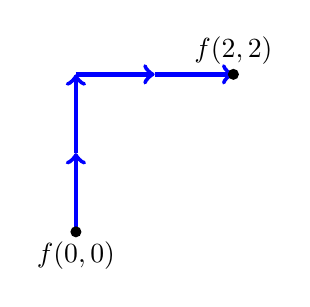
\begin{tikzpicture}
                \thegrid
                \draw[ultra thick, blue, ->] (0,0) -- (0,1);
                \draw[ultra thick, blue, ->] (0,1) -- (0,2);
                \draw[ultra thick, blue, ->] (0,2) -- (1,2);
                \draw[ultra thick, blue, ->] (1,2) -- (2,2);
                \fill[black]
                    (0,0) circle (2pt) node[below] {$f(0,0)$}
                    (2,2) circle (2pt) node[above] {$f(2,2)$};
            \end{tikzpicture}&
            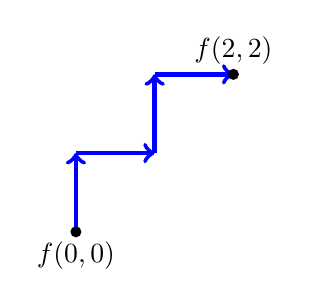
\begin{tikzpicture}
                \thegrid
                \draw[ultra thick, blue, ->] (0,0) -- (0,1);
                \draw[ultra thick, blue, ->] (0,1) -- (1,1);
                \draw[ultra thick, blue, ->] (1,1) -- (1,2);
                \draw[ultra thick, blue, ->] (1,2) -- (2,2);
                \fill[black]
                    (0,0) circle (2pt) node[below] {$f(0,0)$}
                    (2,2) circle (2pt) node[above] {$f(2,2)$};
            \end{tikzpicture}&
            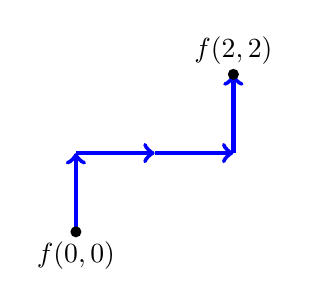
\begin{tikzpicture}
                \thegrid
                \draw[ultra thick, blue, ->] (0,0) -- (0,1);
                \draw[ultra thick, blue, ->] (0,1) -- (1,1);
                \draw[ultra thick, blue, ->] (1,1) -- (2,1);
                \draw[ultra thick, blue, ->] (2,1) -- (2,2);
                \fill[black]
                    (0,0) circle (2pt) node[below] {$f(0,0)$}
                    (2,2) circle (2pt) node[above] {$f(2,2)$};
            \end{tikzpicture}\\
            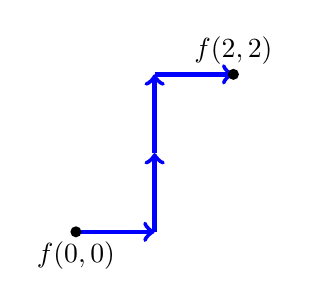
\begin{tikzpicture}
                \thegrid
                \draw[ultra thick, blue, ->] (0,0) -- (1,0);
                \draw[ultra thick, blue, ->] (1,0) -- (1,1);
                \draw[ultra thick, blue, ->] (1,1) -- (1,2);
                \draw[ultra thick, blue, ->] (1,2) -- (2,2);
                \fill[black]
                    (0,0) circle (2pt) node[below] {$f(0,0)$}
                    (2,2) circle (2pt) node[above] {$f(2,2)$};
            \end{tikzpicture}&
            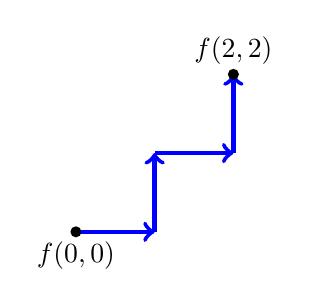
\begin{tikzpicture}
                \thegrid
                \draw[ultra thick, blue, ->] (0,0) -- (1,0);
                \draw[ultra thick, blue, ->] (1,0) -- (1,1);
                \draw[ultra thick, blue, ->] (1,1) -- (2,1);
                \draw[ultra thick, blue, ->] (2,1) -- (2,2);
                \fill[black]
                    (0,0) circle (2pt) node[below] {$f(0,0)$}
                    (2,2) circle (2pt) node[above] {$f(2,2)$};
            \end{tikzpicture}&
            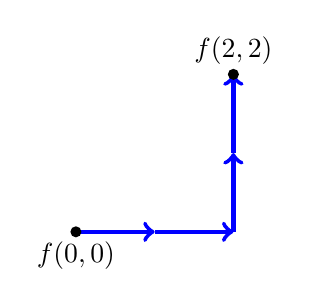
\begin{tikzpicture}
                \thegrid
                \draw[ultra thick, blue, ->] (0,0) -- (1,0);
                \draw[ultra thick, blue, ->] (1,0) -- (2,0);
                \draw[ultra thick, blue, ->] (2,0) -- (2,1);
                \draw[ultra thick, blue, ->] (2,1) -- (2,2);[]
                \fill[black]
                    (0,0) circle (2pt) node[below] {$f(0,0)$}
                    (2,2) circle (2pt) node[above] {$f(2,2)$};
            \end{tikzpicture}
        \end{tabular}
    \end{center}
    \caption{The six constraints on the computation of $f(2, 2)$.
%    $\shift 2 \shift 2 \shift 1 \shift 1 f = \shift 2 \shift 1 \shift 2 \shift 1 f = \shift 2 \shift 1 \shift 1 \shift 2 f = \shift 1 \shift 2 \shift 2 \shift 1 f = \shift 1 \shift 2 \shift 1 \shift 2 f = \shift 1 \shift 1 \shift 2 \shift 2 f$.
    }
    \label{fig:polyrec constraints}
\end{figure}

\paragraph{Multivariate \CDA~series}
%
In the second problem, we consider the notion of
\emph{constructible differentially algebraic} (\CDA) power series in commuting variables~\cite{BergeronReutenauer:EJC:1990}.
%
They were introduced in the multivariate context by Bergeron and Sattler~\cite{BergeronSattler:TCS:1995},
as solutions of systems of \emph{polynomial differential equations} of a restricted form (\cf~\cref{sec:CDA algebra} for details).
%
Such systems may not have solutions
and deciding whether this is the case is open~\cite[Remark 27]{Clemente:CONCUR:2024}.
%
Solvability of polynomial differential equations is undecidable
by a result of Denef and Lipshitz~\cite[Theorem 4.11]{DenefLipshitz:1984}
(\cref{rem:undecidability of solvability}),
and thus it is not clear whether \CDA~series have a decidable syntax.
%
We overcome this issue by showing that commutativity of shuffle automata
can be used to decide whether \CDA~systems are solvable~(\cref{thm:decidability of CDA solvability}),
thus answering the open question positively.

\subsection*{Organisation}
%
In the next section~\cref{sec:preliminaries} we present some preliminaries,
followed in~\cref{sec:commutativity} by a proof of~\cref{thm:commutativity for effective prevarieties}.
%
In \cref{sec:recognisable} we recall some known results about finite weighted automata,
which will help to put the following results in perspective.
%
Polynomial automata will be studied in~\cref{sec:Hadamard},
followed by shuffle automata in~\cref{sec:shuffle},
and infiltration automata in~\cref{sec:infiltration}.
%
(Thus the proof of \cref{thm:main theorem} is spread over these three sections.)
%
In the last section, an important remark shows that our techniques do not only solve the zeroness, equality, and commutativity problems,
but in fact we can construct a finite representation for the \emph{effective algebraic variety}
of all initial conditions ensuring zeroness, equality, resp., commutativity (\cref{rem:effective algebraic varieties}).
%
% In~\cref{sec:extensions} we discuss some extensions of our results.
% In~\cref{sec:mixed product} we discuss an extension of our results where Hadamard, shuffle, and infiltration products can co-exist in the same model.

This paper is an extended version of~\cite{Clemente:LICS:2025}.
%
In comparison to~\cite{Clemente:LICS:2025},
we have included more details and all interesting proofs.
%
Moreover, we provide the complete development for infiltration automata (\cref{sec:infiltration}),
which before was just sketched.
%
We have also introduced a new closure property,
namely closure under left anti-derivatives (\cref{sec:commutativity}),
which allows us to provide a very simple argument showing that the equality prolem
reduces back to the commutativity problem.
%
The preliminary section \cref{sec:recognisable} providing a gentle introduction in the linear case is also new.
%!TEX root main.tex
\section{Preliminaries}
\label{sec:preliminaries}

% To simplify notation,
% we assume that function application binds tighter than any other operation.
% %
% Sometimes we use redundant parentheses for clarity or emphasis.
%
% Let $\Q$ be the field of rational numbers.
%
We say that a structure (such as a class of series, a class of languages, an algebra, etc...)
is \emph{effective} if its elements can be finitely represented (with a decidable syntax),
equality between elements can be decided based on their representations,
and all the structure operations can be carried over algorithmically.
%
For instance the class of regular languages is effective,
since they can be represented by finite automata (amongst many other options)
and language equality is decidable.
%
Most results in the paper hold for any field,
however for computability considerations we need to restrict ourselves to effective fields.
%
For concreteness, we consider the field of rational numbers $\Q$,
however all our results hold for other effective fields,
such as the real numbers $\R$ or the complex numbers $\C$.

% lax begin Lax619925.Series
\paragraph{Series.}

Let $\Sigma = \set{a_1, \dots, a_d}$ be a finite input alphabet.
% We denote letters from $\Sigma$ by $a, b, c$.
% %
We denote by $\Sigma^*$ the set of \emph{finite words} over $\Sigma$,
a monoid under the operation of concatenation,
with neutral element the empty word $\e$.
% %
% We use $u, v, w$ to denote words in $\Sigma^*$.
% %
The main object of study in this paper are \emph{series} over $\Q$,
which are mappings $\Sigma^* \to \Q$.
%
These are sometimes called \emph{weighted languages}
and are denoted by $\series \Q \Sigma$.
%
We refer to~\cite{BerstelReutenauer:CUP:2010} for a general introduction.
%
We use $f, g, h$ to denote series in $\series \Q \Sigma$,
and we write a series $f$ as $\sum_{w \in \Sigma^*} f_w \cdot w$,
where the value of $f$ at $w$ is $f_w \in \Q$.
%
We also write $\coefficient w f$ for $f_w$.
%
The \emph{support} of a series $f$
is the set of words $w$ such that $f_w \neq 0$.
%
A \emph{polynomial} is a series with finite support. 
%
Thus, $3aab - \frac 5 2 bc$ is a polynomial
and $1+a+a^2 + \cdots$ is a series but not a polynomial.

The set of series is equipped with a variety of operations.
%
It carries the structure of a vector space,
with \emph{zero} $\zero$,
\emph{scalar multiplication} $c \cdot f$ with $c \in \Q$,
and \emph{addition} $f + g$ all defined element-wise by
%
\begin{align*}
    \coefficient w \zero := 0, \qquad
    \coefficient w {(c \cdot f)} := c \cdot \coefficient w f, \qquad \text{and} \qquad
    \coefficient w {(f + g)} := \coefficient w f + \coefficient w g,
    \qquad \forall w \in \Sigma^*.
\end{align*}
%
This vector space is equipped with two important families of linear maps,
called \emph{left} and \emph{right derivatives}
$\deriveleft a, \deriveright a : \series \Q \Sigma \to \series \Q \Sigma$,
for every $a \in \Sigma$.
%
They are the series analogues of language quotients:
%
For every series $f \in \series \Q \Sigma$,
they are defined element-wise by
%
\begin{align*}
    \coefficient w {(\deriveleft a f)}
        &:= \coefficient {a \cdot w} f,
    \qquad\text{resp.,}\qquad
    \coefficient w {(\deriveright a f)}
        := \coefficient {w \cdot a} f,
    \qquad \forall w \in \Sigma^*.
\end{align*}
%
The following elementary observation will be very useful.
%
\begin{restatable}[Left and right derivatives commute]{lemma}{leftRightComm}
    \label{lem:derive left right commutativity}
    For every two letters $a, b \in \Sigma$,
    we have $\deriveleft a \circ \deriveright b = \deriveright b \circ \deriveleft a$.
\end{restatable}
\noindent
(By $\deriveleft a \circ \deriveright b$ we mean the \emph{composition} of the two derivatives,
which is the function mapping a series $f$ to the series $\deriveleft a \deriveright b f$.
We avoid writing parenthesis for function application when possible.)
%
% \begin{proof}
%     This follows from associativity of concatenation of finite words:
%     Indeed, for any series $f \in \series \Q \Sigma$ and word $w \in \Sigma^*$ we have,
%     \begin{align*}
%         \coefficient w {\deriveleft u \deriveright v f}
%             &= \coefficient {uw} {\deriveright v f}
%             = \coefficient {uwv} f, \quad \text{ and } \\
%         \coefficient w {\deriveright v \deriveleft u f}
%             &= \coefficient {wv} {\deriveright v f}
%             = \coefficient {uwv} f. \qedhere
%     \end{align*}
% \end{proof}
%
% We will later equip series with several bilinear multiplication operations,
% turning them into algebras.
%
% These operations will be defined later in the releavant sections.
%
% We don't need this
% \paragraph{Concatenation product (Cauchy product)}
%
% The \emph{concatenation product} of two series $f, g$
% is the series $f \cdot g$ \st~for every input word $w$ we have
% %
% \begin{align*}
%     \coefficient w {(f \cdot g)} := \sum_{w = u \cdot v} f_u \cdot g_v,
% \end{align*}
% %
% where the sum runs over all finite words $u, v \in \Sigma^*$.
% %
% Note that we have overloaded the symbol ``$\cdot$''
% to denote both the concatenation of words and of series.
%
% \paragraph{Shuffle product}
% \label{sec:shuffle product}
% The \emph{shuffle} of two words $u, v$ is the polynomial $u \shuffle v \in \ncpoly \Q \Sigma$,
% which is defined by induction on the length of words as follows:
% %
% \begin{align*}
%     u \shuffle \e
%         &:= \e \shuffle u := u, \\
%     (a \cdot u) \shuffle (b \cdot v)
%         &:= a \cdot (u \shuffle (b\cdot v)) + b \cdot ((a \cdot u) \shuffle v).
% \end{align*}
% %
% For instance, $ab \shuffle c = cab + acb + abc$ and $a \shuffle a = 2aa$.
% %
% This operation is lifted on series $f, g$ by distributivity:
% $f \shuffle g := \sum_{u, v \in \Sigma^*} f_u \cdot g_v \cdot (u \shuffle v)$.
% %
% We will come back to the shuffle product and its properties in \cref{sec:shuffle}.
%
Derivatives are extended to all finite words homomorphically:
$\deriveleft \e f := f$ and $\deriveleft {a \cdot w} f := \deriveleft w (\deriveleft a f)$
for all $a \in \Sigma$ and $w \in \Sigma^*$ (note that the order is reversed);
similarly for right derivatives.
% lax end
% lax begin Lax619925.Prevariety
\paragraph{Prevarieties of series.}
% We now recall an important notion from the theory of series.
%
Let $\SS$ be a class of series,
and for an alphabet $\Sigma$ let $\SS_\Sigma$ the subset of $\SS$
consisting of series over input alphabet $\Sigma$. %of the form $\series \Q \Sigma$.
%
We require that $\SS_\Gamma \supseteq \SS_\Sigma$ for every alphabet $\Gamma \supseteq \Sigma$.
%
A class of series $\SS$ is a \emph{prevariety} %(\cf~\cite[Sec.~III.1]{Reutenauer_1980})
if the following two conditions hold, for every alphabet $\Sigma$:
%
\begin{enumerate}[label=\textbf{(V.\arabic*)}]
    
    \item \label{prevariety:A}
    $\SS_\Sigma$ is a vector space over $\Q$.

    \item \label{prevariety:B}
    Closure under derivatives:
    For every series $f \in \SS_\Sigma$ and letter $a \in \Sigma$,
    the series $\deriveleft a f$ and $\deriveright a f$ are in $\SS_\Sigma$.

\end{enumerate}
%
(A \emph{variety}, as introduced by Reutenauer,
is a prevariety which satisfies an additional condition (\cf~\cite[Sec.~III.1]{Reutenauer_1980});
we will not need this notion in the rest of the paper.)
% \begin{enumerate}[label=\textbf{(V.\arabic*)}]
%     \setcounter{enumi}{2}
%     \item \label{prevariety:C}
%     For every series $f \in \SS_\Sigma$
%     and algebra homomorphism%
%     \footnote{
%         The corresponding requirement in \cite[Sec.~III.1]{Reutenauer_1980}
%         demands closure \wrt~algebra homomorphisms of the form $\varphi \in \series \Q \Gamma \to \series \Q \Sigma$.
%         %
%         However $f \circ \varphi$ may not be defined when $\varphi$ produces series with infinite supports.
%         For instance take $f = \varphi(a) = 1 + a + a^2 + \cdots$.
%         Then $(f \circ \varphi)(a) = \inner f {\varphi(a)} = 1 + 1 + \cdots$ is not defined.
%         %
%         For this reason $\varphi$ needs to be restricted to be a homomorphism of series with finite supports.
%     }
%     $\varphi : \ncpoly \Q \Gamma \to \ncpoly \Q \Sigma$,
%     % $\varphi \in \series \Q \Gamma \to \series \Q \Sigma$,
%     % $\varphi : \Gamma^* \to \series \Q \Sigma$,
%     the series $f \circ \varphi$ is in $\SS_\Gamma$.
% \end{enumerate}
% %
% In the rest of the paper we will need only the notion of prevariety.
%
The \emph{equality problem} for a prevariety of series $\SS$ is the following decision problem:
Given (finite representations of) two series $f, g \in \SS$, is it the case that $f = g$?
%
In the special case when $g = \zero$ we obtain the \emph{zeroness problem}.
%
A class of series $\SS$ is an \emph{effective prevariety} if it is a prevariety,
and moreover
%
\begin{enumerate}
    \item Every series in $\SS$ admits a decidable finite presentation.
    \item The closure properties \cref{prevariety:A} and \cref{prevariety:B} %in the definition of prevariety
    can be carried over algorithmically by manipulating finite presentations.
    \item The equality problem is decidable for series in $\SS$.
\end{enumerate}
%
% The notion of effective variety is defined in the expected way.
%
\noindent
% In the first point, we do not care about the specific finite representation of a series,
% but only that it can be finitely represented.
% For instance, regular languages are finitely represented by finite automata, regular expressions, or formulas in monadic second-order logic.
% %
%(By a \emph{finite presentation} for series we mean a concrete syntax
%in the same sense, \eg, finite automata are finite presentations for regular languages.)
%
Thanks to the equivalence $f = g \iff f - g = \zero$ and~\cref{prevariety:A},
the notion of effective prevariety does not change if we replace the third condition above
with the following seemingly weaker one:
%
\begin{enumerate}
    \item[3')] the zeroness problem is decidable for series in $\SS$.
\end{enumerate}
%
\noindent
For instance, the class of rational series is an effective prevariety~\cite[Sec.~III.2.b]{Reutenauer_1980},
as we recall later in section~\cref{sec:recognisable}.
% lax end
\section{Commutativity problem}
\label{sec:commutativity}
% lax begin Lax619925.Commutativity

We introduce the main problem that we study.
%
The \emph{commutative image} of a word $w \in \Sigma^*$ (sometimes called \emph{Parikh image})
over a totally ordered alphabet $\Sigma = \set{a_1, \dots, a_d}$
is the vector $\Parikh w := \tuple{\multiplicity {a_1} w, \dots, \multiplicity {a_d} w} \in \N^d$,
where $\multiplicity {a_j} w$ is the number of occurrences of $a_j$ in $w$.
%
For two words $u, v$ we write $u \sim v$ if they have the same commutative image,
\ie, one word can be obtained from the other by permuting the positions of letters.
%
For instance, $a_1a_1a_2 \sim a_1a_2a_1 \sim a_2a_1a_1$,
since the commutative image of all three words is $\tuple{2, 1} \in \N^2$.
%
A series $f \in \series \Q \Sigma$ is \emph{commutative} 
(called \emph{échangeable} in~\cite{Fliess:1981})
if for every two words $u, v \in \Sigma^*$ with the same commutative image $u \sim v$,
the series produces the same value $f_u = f_v$.

On the face of it, commutativity demands to check infinitely many equalities.
%
Our simple, but crucial observation is that it can be characterised by finitely many equations.
%
Clearly, if $f$ is commutative, then for every input symbols $a, b \in \Sigma$ we have
%
\begin{align}
    \label{eq:swap}
    \tag{\textsf{swap}}
    \deriveleft a \deriveleft b f &= \deriveleft b \deriveleft a f, \quad \text{ and } \\
    \label{eq:rotate}
    \tag{\textsf{rotate}}
    \deriveleft a f &= \deriveright a f.
\end{align}
%
Indeed, the first equation corresponds to exchanging the first two input letters $abw \sim baw$,
and the second equation corresponds to a rotation $aw \sim wa$.
%
Since swaps and rotations suffice to generate all commutatively equivalent words,
we obtain the following characterisation.
%
\begin{lemma}[Characterisation of commutativity]
    \label{lem:commutativity}
    A series $f \in \series \Q \Sigma$ is commutative if, and only if,
    it satisfies equations~\cref{eq:swap} and \cref{eq:rotate},
    for every $a, b \in \Sigma$.
\end{lemma}
%
\noindent
Thanks to \cref{lem:commutativity},
commutativity is decidable for effective prevarieties of series.
%
Indeed, if $\SS$ is a prevariety and $f \in \SS$,
then $\deriveleft a f, \deriveright a f, \in \SS$,
as well as all the other series mentioned in \cref{eq:swap,eq:rotate}.
%
By effectiveness, we can construct finite representations for these series and decide the equality tests.
%
This observation will allow us to decide commutativity for rich classes of series
for which the commutativity problem is nontrivial.
%
\thmCommutativityForPrevarieties*

\begin{remark}
    \Cref{thm:commutativity for effective prevarieties} allows us
    to reduce commutativity to finitely many equality tests.
    %
    The observation that commutativity can be characterised by finitely many equations is certainly not novel.
    For instance, in the context of formal verification
    one could find an analogous statement in~\cite[Prop.~2]{ChenSongWu:CAV:2016}.
\end{remark}

The three classes of series that we consider in~\cref{sec:Hadamard,sec:shuffle,sec:infiltration} will turn out to be effective prevarieties,
and thus commutativity is decidable for them.
%
One may wonder whether equality reduces back to commutativity, so that the two problems are in fact inter-reducible.
This will indeed be the case, thanks to an additional closure property that we introduce next.
%
We say that a series $g \in \series \Q \Sigma$
is a \emph{left anti-derivative} of a tuple of series $f = \tuple{f_a}_{a \in \Sigma} \in \series \Q \Sigma^\Sigma$
if $\deriveleft a g = f_a$ for all $a \in \Sigma$.
%
Clearly, once we fix the initial condition $g_\e \in \Q$,
anti-derivatives are unique.
%
A class of series $\SS$ is \emph{closed under left anti-derivatives} if
whenever $g$ is a left anti-derivative of a tuple of series $f$ from $\SS_\Sigma$,
then $g$ is also in $\SS_\Sigma$.
%
\begin{restatable}{lemma}{commutativityGeneralisesEquality}
    \label{lem:equality reduces to commutativity}
    Le $\SS$ be an effective prevariety of series, except that the equality problem is not assumed to be decidable.
    If $\SS$ is effectively closed under left anti-derivatives,
    then the zeroness problem effectively reduces to the commutativity problem.
\end{restatable}
\begin{proof}
    Consider a finite alphabet $\Sigma$ and a series $f \in \SS_\Sigma$ over $\Sigma$.
    Let $a, b \not \in \Sigma$ be two fresh letters not in $\Sigma$
    and define the enlarged alphabet $\Gamma := \Sigma \cup \set{a, b}$.
    %
    Let $g \in \SS_\Gamma$ be the unique series such that $g_\e = g_x = 0$ for all $x \in \Gamma$,
    and, for every $x, y \in \Gamma$,
    %
    \begin{align*}
        \deriveleft y \deriveleft x g =
        \begin{cases}
            f
                &\text{if } x = a, y = b, \text{ and } \\
            \zero
                &\text{otherwise.}
        \end{cases}
    \end{align*}
    %
    Since $\SS$ is closed under anti-derivatives, $g$ is in $\SS_\Gamma$.
    %
    We claim that $g$ is commutative if, and only if, $f = \zero$.
    The ``if'' direction is clear since $f = \zero$ implies $g = \zero$, which is commutative.
    For the ``only if'' direction, assume that $f \neq \zero$, so that there is a word $w \in \Sigma^*$ in its support $f(w) \neq 0$.
    Then $g(abw) = f(w) \neq 0$ however $g(baw) = 0$,
    and thus $g$ is not commutative.
\end{proof}

In~\cref{sec:Hadamard,sec:shuffle,sec:infiltration}
we leverage~\cref{thm:commutativity for effective prevarieties,lem:equality reduces to commutativity}
for three expressive classes of series, together with respective applications.
%
%Some extensions will be mentioned in the last section~\cref{sec:extensions}.
% lax end
%!TEX root main.tex
\section{Linearly-finite series and recognisable series}
\label{sec:recognisable}
% lax begin Lax619925.Recognisable

This brief section does not contain any new results,
however it will be instructive in comparison with the stronger results
developed in~\cref{sec:Hadamard,sec:shuffle,sec:infiltration}.
%
%Recall that a \emph{vector space} over the rationals $\Q$ is a tuple $\V = \tuple{V; %\zero, \cdot, +}$
%consisting of the zero vector $\zero$, a scalar product $\cdot : \Q \times V \to V$a
%and compatible addition operation $+ : V \times V \to V$.
%
% A \emph{linear transition system} consists of a set $V$ simultaneously carrying the structure of a weighted transition system and a vector space.
% %
% Formally, a \emph{linear transition system} (\LTS) is a tuple
% $\A = \tuple{\Sigma, V; F, \delta; \zero, \cdot, +}$
% where $\T = \tuple {\Sigma, V; F, \delta}$ is a \WTS\-
% and $\V = \tuple{V; \zero, \cdot, +}$ is a vector space (over the rationals $\Q$).
% %
% Moreover, we require that the output mapping $F : V \to \Q$
% and the transition functions $\delta_a : V \to V$ (for all $a \in \Sigma$) are linear.
% %
% For instance, series with left derivatives
% $\Tleft = \tuple{\Sigma, \series \Q \Sigma; \e, \deriveleft {}; \zero, \cdot, +}$
% form a linear transition system.

\paragraph{Linearly-finite series.}

We recall a semantic mechanism to define classes of series
that will be useful in the rest of the paper in comparison to more general classes.
%
Given a set of series $F \subseteq \series \Q \Sigma$,
let their \emph{linear span}, denoted by $\linearspan \Q F$,
be the set of finite linear combinations of series from $F$,
with coefficients from $\Q$.
%
In other words, elements of this set are of the form $c_1 \cdot f_1 + \cdots + c_n \cdot f_n$
for some $f_1, \dots, f_n \in F$ and $c_1, \dots, c_n \in \Q$.
%
It is easy to see that $\linearspan \Q F$ is a vector space over $\Q$ containing $F$,
and in fact it is the smallest such vector space.
%
Sets of series of the form $\linearspan \Q {f_1, \dots, f_k}$ are called \emph{finitely generated},
with \emph{generators} $f_1, \dots, f_k$.
%
We say that a series $f \in \series \Q \Sigma$ is \emph{linearly finite}
if it belongs to a finitely generated $\Q$-vector space of series
closed under left derivatives $\deriveleft a$, $a \in \Sigma$.
%
In other words, $f$ is linearly finite when there are generators $f_1, \dots, f_k \in \series \Q \Sigma$ \st:
%
\begin{enumerate}[label=\textbf{(R.\arabic*)}]
    \item \label{linearly_finite:1} $f \in \linearspan \Q {f_1, \dots, f_k}$ and
    \item \label{linearly_finite:2} $\deriveleft a f_i \in \linearspan \Q {f_1, \dots, f_k}$
    for every $a \in \Sigma$ and $1 \leq i \leq k$,
\end{enumerate}

\begin{remark}
    We would get the same class if we additionally required that the generators
    are obtained from $f$ itself by a finite number of left derivatives.
    %
    In other words, we could take the generators to be of the form $f_i = \deriveleft {w_i} f$ for some words $w_i \in \Sigma^*$.
    %
    Since this will not be the case for the more general classes of series that we will consider in the rest of the paper,
    we have chosen the definition above.
\end{remark}

\begin{lemma}
    \label{lem:recognisable closure properties}
    The class of linearly finite series is effectively closed under
    scalar product, addition, left derivatives and anti-derivatives.
\end{lemma}
%
\begin{proof}
    Closure under scalar product follows from the definition of linear span.
    %
    Regarding closure under addition, let $f, g$ be linearly finite series with generators $F$, resp., $G$.
    Then $f + g$ is linearly finite with generators $F \cup G$.
    %
    Closure under left derivatives holds by design:
    If $f$ is linearly finite with generators $G$,  %= \set {f_1, \dots, f_k}$,
    then for every $a \in \Sigma$ the series $\deriveleft a f$ is also linearly finite with the same set of generators.
    %
    % Indeed, by \cref{linearly_finite:1} $f$ is of the form $\sum_{i = 1}^k c_i \cdot f_i$ for some $c_i \in \Q$,
    % and thus by linearity of left derivative we have $\deriveleft a f = \sum_{i = 1}^k c_i \cdot \deriveleft a f_i$.
    % %
    % But now by \cref{linearly_finite:2} we can replace each $\deriveleft a f_i$ by a linear combination of the generators,
    % showing that $\deriveleft a f$ is in the linear span of $G$.
    %
    Finally, for closure under anti-derivatives
    consider linearly finite series $f_1, \dots, f_d$ with generators, resp., $G_1, \dots, G_d$
    \st~$\deriveleft {a_j} f = f_j$ for every $1 \leq j \leq d$.
    %
    Then $f$ is linearly finite with generators $\set {f, f_1, \dots, f_d} \cup G_1 \cup \cdots \cup G_d$.
\end{proof}

The class of linearly finite series is also closed under right derivatives,
however we will obtain this from a stronger closure property, namely closure under reversal.
%
To show the latter, we will use a stronger representation for linearly finite series,
which we recall next.

\paragraph{Linear representations.}

A \emph{linear representation} is a tuple $\tuple{\Sigma, k, x, y, M}$,
where $\Sigma = \set{a_1, \dots, a_d}$ is a finite alphabet,
$k \in \N$ is the \emph{dimension} of the representation,
$x \in \Q^{1 \times k}$ is a row vector of \emph{initial weights},
$y \in \Q^{k \times 1}$ is a column vector of \emph{final weights},
and $M : \Sigma \to \Q^{k \times k}$ is the \emph{transition function},
assigning to each input letter $a \in \Sigma$ a transition matrix $M(a) \in \Q^{k \times k}$.
%
The transition function $M$ is extended homomorphically to all input words $M : \Sigma^* \to \Q^{k \times k}$
by $M(\e) := I_k$ (the $k \times k$ identity matrix)
and $M(a \cdot w) := M(a) \cdot M(w)$ for every $a \in \Sigma$ and $w \in \Sigma^*$.
%
A linear representation \emph{recognises} the series $f \in \series \Q \Sigma$
mapping an input word $w \in \Sigma^*$ to $\coefficient w f := x \cdot M(w) \cdot y$.
%
A series is \emph{recognisable} if it is recognised by some linear representation.
%
The following coincidence result is classical (\cf~\cite[Proposition~5.1]{BerstelReutenauer:CUP:2010}).
%
\begin{lemma}
    A series is recognisable if, and only if, it is linearly finite.
\end{lemma}
%
% \begin{proof}
%     For the ``only if'' direction, assume that $f$ is recognisable.
%     Let $\tuple{\Sigma, k, x, y, M}$ be a linear representation recognising $f$.
%     %
%     Consider the series $g := M \cdot y \in \series {\Q^{k \times 1}} \Sigma$.
%     %
%     In other words, $g_i(w)$ is the $i$-th component of the vector $M(w) \cdot y$.
%     %
%     Then $f$ is linearly finite with generators $g_1, \dots, g_k$.
%     Indeed, $f = u \cdot M \cdot y = \sum_{i = 1}^k u_i \cdot g_i$, showing~\cref{linearly_finite:1}.
%     Moreover, $\deriveleft a g \in \series {\Q^{k \times 1}} \Sigma$ is the series that maps an input word $w$ to
%     %
%     \begin{align*}
%         g(a \cdot w)
%         = M(a) \cdot M(w) \cdot y
%         = M(a) \cdot g(w),
%     \end{align*}
%     %
%     and thus all components of $\deriveleft a g = M(a) \cdot g$ are in the linear span of the generators.
%
%     For the other direction, assume that $f$ is linearly finite
%     with generators $g = \tuple{g_1, \dots, g_k} \in \series \Q \Sigma^{k \times 1}$.
%     %
%     Since $f$ is in the linear span of the generators by~\cref{linearly_finite:1},
%     there are coefficients $x \in \Q^{1 \times k}$ \st~$f = x \cdot g$.
%     %
%     For every input symbol $a \in \Sigma$,
%     by~\cref{linearly_finite:2} each component of $\deriveleft a g$ is in the linear span of the generators,
%     and thus there is a matrix $M(a) \in \Q^{k \times k}$ \st~$\deriveleft a g = M(a) \cdot g$.
%     %
%     Finally, let $y = g(\e) \in \Q^{k \times 1}$ be the vector of constant terms of the generators.
%     %
%     Then $f$ is recognised by the linear representation $\tuple{\Sigma, k, x, y, M}$.
%     %
%     \begin{claim*}
%         We have $g = M \cdot y$.
%     \end{claim*}
%     \begin{claimproof}
%         We proceed by coinduction.
%         In the base case, we have $g(\e) = y = M(\e) \cdot y$.
%         %
%         In the coinductive case we have 
%         $\deriveleft a g = M(a) \cdot g = M(a) \cdot M \cdot y = (\deriveleft a M) \cdot y = \deriveleft a (M \cdot y)$.
%     \end{claimproof}
%     %
%     Thanks to the claim we have $f = x \cdot g = x \cdot M \cdot y$,
%     as required.
% \end{proof}
%
\noindent
Thanks to the lemma above,
recognisable series are closed under the operations from~\cref{lem:recognisable closure properties}.
%
The advantage of linear representations is that they make it possible to show stronger closure properties,
as we now demonstrate.
%
The \emph{reversal} of series $f \in \series \Q \Sigma$ is the series $\reversal f \in \series \Q \Sigma$
which reverses the order of the letters in the input.
%
That is, for every input word $w \in \Sigma^*$ we have $\coefficient w {(\reversal f)} := \coefficient {\reversal w} f$,
where $\reversal w$ is the word obtained from $w$ by reversing the order of its letters.
%
For instance, $\reversal {(a b c)} = c b a$.
%
Note that reversal is an endomorphism on the vector space of series.
%
\begin{lemma}
    If $f \in \series \Q \Sigma$ is recognisable, then $\reversal f$ is also recognisable.
\end{lemma}
%
\begin{proof}
    Let $f$ be recognised by a linear representation $\tuple{\Sigma, k, x, y, M}$.
    Then its reversal $\reversal f$ is recognised by the linear representation $\tuple{\Sigma, k, \transpose y, \transpose x, \transpose M}$,
    where $\transpose M$ is the transpose of $M$, and similarly for $\transpose y, \transpose x$.
    %
    Indeed, for every input word $w \in \Sigma^*$ we have
    %
    $
        \coefficient w {(\reversal f)}
        = \coefficient {\reversal w} f
        = x \cdot M(\reversal w) \cdot y
        = x \cdot \transpose {(\transpose M(w))} \cdot y
        = \transpose y \cdot \transpose M(w) \cdot \transpose x
    $.
\end{proof}
%
\noindent
Notice that it is not so clear how to prove closure under reversal
solely based on the definition of linearly finite series.
%
Since recognisable series are closed under left derivatives and reversal,
by double reversal $\deriveright a f = \reversal {(\deriveleft a \reversal f)}$
we obtain closure under right derivatives as well.
%
\begin{corollary}
    \label{cor:recognisable derive right}
    If $f$ is recognisable then $\deriveright a f$ is also recognisable.
\end{corollary}
% \begin{proof}
    % Let $f_1, \dots, f_k$ be generators for $f$.
    % We adjoin new generators $\deriveright a f_i$
    % for every $a \in \Sigma$ and $1 \leq i \leq k$.
    % %
    % Since $f$ is in the linear span of the $f_i$'s,
    % we have that $\deriveright a f$ is in the linear span of the $\deriveright a f_i$'s,
    % thus the first condition is satisfied.
    % %
    % Now consider $\deriveleft a \deriveright b f_i$.
    % Since left and right derivatives commute by~\cref{lem:derive left right commutativity},
    % we have $\deriveleft a \deriveright b f_i = \deriveright b \deriveleft a f_i$.
    % %
    % But $\deriveleft a f_i$ is in the linear span of the $f_i$'s.
    % Since right derivation is linear,
    % $\deriveright b \deriveleft a f_i$ is in the linear span of the $\deriveright b f_i$'s.
    % \qedhere
% \end{proof}

\begin{theorem}
    The class of recognisable (= linearly finite) series is an effective prevariety.
    In particular, the commutativity problem is decidable.
\end{theorem}

% \paragraph{Minimisation of linear representations.}
% %
% If a rational series is commutative,
% then in a minimal linear representation the transition matrices commute pairwise.

\paragraph{Towards more general classes.}

In the next sections~\cref{sec:Hadamard,sec:shuffle,sec:infiltration}
we will consider classes of series which generalise the recognisable ones.
%
In each case, the more general class will be obtained by considering a notion of product of series,
thus moving from a vector space structure to a more general algebra structure.
%
The basic closure properties as in~\cref{lem:recognisable closure properties} will follow from first principles.
%
Decidability of the zeroness problem will be obtained as an application of Hilbert finite basis theorem
for finitely generated polynomial algebras with finitely many variables.
%
The price to pay is that such classes of series will not be closed under reversal in general.
%
Consequently, in order to show that they are prevarieties
we will need to show closure under right derivatives by other means.
% lax end
%!TEX root main.tex
\section{Hadamard automata and Hadamard-finite series}
\label{sec:Hadamard}

In this section, we study a weighted model of computation strongly related to polynomial automata
and the class of series its recognises.
%
We begin in~\cref{sec:Hadamard:preliminaries} with some mathematical preliminaries.
%
In~\cref{sec:Hadamard-finite series} we define Hadamard-finite series, generalising the recognisable series,
and present their closure properties.
%
Hadamard automata are defined and studied in~\cref{sec:Hadamard automata},
where they are shown to recognise precisely the Hadamard-finite series.
%
This leads to the main result of the section:
Hadamard-finite series constitute an effective prevariety~(\cref{thm:Hadamard prevariety})
and thus the commutativity problem is decidable for this model\-
(\cref{thm:Hadamard-finite series - decidable commutativity}).
%
We conclude in~\cref{sec:multivariate polyrec} with an application of the commutativity problem
to a class of multivariate number sequences defined by polynomial recursions~(\cref{thm:polyrec consistency}).

\subsection{Preliminaries}
\label{sec:Hadamard:preliminaries}

\subsubsection{Difference algebra}
\label{sec:difference algebra}

Let $\A = \tuple{A; 0, 1, {+}, {*}}$ be an \emph{algebra} (over the field of rational numbers),
that is a vector space equipped with an associative commutative bilinear product
with identity $1$~\cite[Ch.~3, §1]{Bourbaki:Algebra:I:1974}.
%
An algebra \emph{endomorphism} is a linear function $F : A \to A$ \st
%
\begin{align}
    \label{eq:endomorphism}
    \tag{endomorphism rule}
    F(1) = 1
        \qquad\text{and}\qquad
        F(\alpha * \beta) = F \alpha * F \beta,
        \quad\text{for all } \alpha, \beta \in A.
\end{align}
%
A \emph{difference algebra}~\cite{RMCohn:DifferenceAlgebra:1965,Levin:DifferenceAlgebra:2008}
is an algebra $\tuple{A; 0, 1, {+}, {*}, (F_j)_{1\leq j\leq d}}$
together with finitely many endomorphisms $F_1, \dots, F_d : A \to A$.
%
Unlike what is usually assumed in the difference algebra literature,
we do not require the $F_i$'s to pairwise commute.
%
Difference algebras will provide the semantic background for the rest of the section.

As an example, consider the algebra of multivariate polynomials
$\tuple{\poly \Q X; 0, 1, {+}, {\cdot}}$,
where $X = \tuple{X_1, \dots, X_k}$ is a tuple of commuting variables.
%
%When the variable names do not matter,
%we sometimes write $\poly \Q k$ instead of $\poly \Q X$.
%
An endomorphism $F$ acts on a polynomial $\alpha \in \poly \Q X$
just by evaluation $F \alpha = \alpha(F(X_1), \dots, F(X_k))$,
and thus it is uniquely defined once we have fixed $F(X_1), \dots, F(X_k) \in \poly \Q X$.
%
% This presentation choice will make it easier to compare homomorphisms
% with shuffles and infiltrations in the upcoming sections.
%
If we fix distinguished endomorphisms $F_1, \dots, F_d$,
then the algebra of polynomials acquires the structure of a difference algebra
$\tuple{\poly \Q X; 0, 1, {+}, {\cdot}, (F_j)_{1 \leq j \leq d}}$.
%
Other examples of difference algebras will be presented in \cref{sec:Hadamard algebra,sec:shift algebra}.

\subsubsection{Hadamard difference algebra}
\label{sec:Hadamard algebra}

We define a product operation on series
which will be central for the development of this section.
%
The \emph{Hadamard product}~\cite{Fliess:1974} of two series $f, g \in \series \Q \Sigma$,
denoted by $f \hadamard g$,
is defined element-wise:
For every $w \in \Sigma^*$,
$\coefficient w (f \hadamard g) := \coefficient w f \cdot \coefficient w g$.
%
For instance, if we have two polynomials $2 \cdot aab - c$ and $3 \cdot aab + b$ (in noncommuting variables),
their Hadamard product is $6 \cdot aab$.
%
This is an associative and commutative operation, it distributes over sum,
and the identity element is the series $\one = \sum_{w\in \Sigma^*} 1 \cdot w$ mapping every word to $1$,
giving rise to the \emph{Hadamard algebra} $\tuple{\series \Q \Sigma; \zero, \one, {+}, {\hadamard}}$.
%
The Hadamard product for series is reminiscent of the notion of \emph{intersection} in language theory
and of \emph{fully synchronous composition} in concurrency theory.

In order to make it easier to compare the Hadamard product
to the shuffle and infiltration products studied later,
we find it convenient to provide the following alternative,
coinductive definition
(\cf~\cite[Definition 8.1]{BasoldHansenPinRutten:MSCS:2017}):
%
For any two series $f, g \in \series \Q \Sigma$,
their Hadamard product $f \hadamard g$
is the unique series \st
%
\begin{align}
    \tag{${\hadamard}$-$\e$}
    \label{eq:hadamard:base}
    \coefficient \e {(f \hadamard g)}
        &= f_\e \cdot g_\e, \\
    \tag{${\hadamard}$-$\deriveleft a$}
    \label{eq:hadamard:step}
        \deriveleft a (f \hadamard g)
        &= \deriveleft a f \hadamard \deriveleft a g,
        \ \forall a \in \Sigma.
\end{align}
%
%Thus it gives rise to the \emph{Hadamard algebra} of series
%$\series \Q \Sigma_{\hadamard} = \tuple{\series \Q \Sigma, {+}, {\hadamard}}$.
%
Equation \cref{eq:hadamard:step} states that left derivatives are endomorphisms \wrt~the Hadamard product.
%
We thus obtain the \emph{Hadamard difference algebra} of series
%\begin{align*}
    $\series \Q \Sigma_{\hadamard} := \tuple{\series \Q \Sigma; \zero, \one, {+}, {\hadamard}, (\deriveleft a)_{a \in \Sigma}}$,
%\end{align*}
which will provide the semantic background
for the forthcoming Hadamard automata.
%
Right derivatives are also Hadamard algebra endomorphisms,
which will be useful later.
% which will be used later in the proof of~\cref{lem:Hadamard closure properties}.
%
\begin{restatable}{proposition}{lemRightDerivationHadamardEndo}
    \label{lem:right derivation Hadamard endomorphism}
    Right derivatives $\deriveright a$ (with $a \in \Sigma$) are Hadamard algebra endomorphisms.
    I.e., they are linear, preserve the multiplicative identity $\deriveright a \one = \one$,
    and commute with Hadamard product:
    %
    \begin{align}
        \tag{${\hadamard}$-$\deriveright a$}
        \label{eq:derive hadamard right}
        \deriveright a (f \hadamard g) = \deriveright a f \hadamard \deriveright a g,
        \quad\forall a \in \Sigma.
    \end{align}
\end{restatable}
%
% \begin{proof}
%     Linearity follows directly from the definition of $\deriveright a$.
%     Equation~\cref{eq:derive hadamard right} could be proved coinductively,
%     however a direct argument suffices since the Hadamard product acts element-wise:
%     For every $w \in \Sigma^*$ and $a \in \Sigma$,
%     %
%     \begin{align*}
%         \coefficient w {\deriveright a (f \hadamard g)}
%         &= \coefficient {wa} {(f \hadamard g)}
%         = \coefficient {wa} f \cdot \coefficient {wa} g
%         = \coefficient w \deriveright a f \cdot \coefficient w \deriveright a g
%         = \coefficient w (\deriveright a f \hadamard \deriveright a g). \qedhere
%     \end{align*}
% \end{proof}

\subsection{Hadamard-finite series}
\label{sec:Hadamard-finite series}

In this section we rely on the structure of the Hadamard algebra
to define a finitely presented class of series.
%
For series $f_1, \dots, f_k \in \series \Q \Sigma$,
let $\poly \Q {f_1, \dots, f_k}_{\hadamard}$ be the smallest Hadamard algebra containing $f_1, \dots, f_k$.
%
Hadamard algebras of this form are called~\emph{finitely generated},
with \emph{generators} $f_1, \dots, f_k$.
%
It is a \emph{difference Hadamard algebra}
if it is additionally closed under the endomorphisms $\deriveleft a$, $a \in \Sigma$.
%
\begin{definition}[Hadamard-finite series]
    \label{def:Hadamard finite}
    A series is \emph{Hadamard finite} if it belongs to a
    finitely generated difference Hadamard algebra.
\end{definition}
%
\noindent
The following lemma will be our working definition of Hadamard-finite series.
%
\begin{restatable}{lemma}{lemHadamardFiniteWorkingDefinition}
    \label{lem:Hadamard finite - working definition}
    A series $f$ is Hadamard finite iff there are generators $f_1, \dots, f_k$ \st:
    %
    \begin{enumerate}
        \item $f \in \poly \Q {f_1, \dots, f_k}_{\hadamard}$.
        %\Ie, there exists a polynomial $p \in \poly \Q {y_1, \dots, y_k}$
        %\st~$f = p(f_1, \dots, f_k)$.

        \item $\deriveleft a f_i \in \poly \Q {f_1, \dots, f_k}_{\hadamard}$
        for every $a \in \Sigma$ and $1 \leq i \leq k$.
        %
        \Ie, there are polynomials $p^{(a)}_i \in \poly \Q {y_1, \dots, y_k}$ \st
        %
        \begin{align}
            \label{eq:Hadamard finite equations}
            \deriveleft a f_i = p^{(a)}_i(f_1, \dots, f_k),
            \quad\text{for all } a \in \Sigma, 1 \leq i \leq k.
        \end{align}
    \end{enumerate}
    %
    Moreover, we can assume without loss of generality that $f$ equals one of the generators $f = f_1$.
\end{restatable}
%
\noindent
We call~\cref{eq:Hadamard finite equations}~a \emph{system of Hadamard-finite equations}.
%
Note that every choice for the constant terms $\coefficient \e {f_i} \in \Q$
extends to a unique series solution of~\cref{eq:Hadamard finite equations}.
%
Consequently, a Hadamard-finite series can be finitely presented by
the constant terms and the polynomials $p_i^{(a)} \in \poly \Q {y_1, \dots, y_k}$.
%
%
\begin{proof}
    If $f$ is Hadamard finite, then the two conditions hold by definition.
    \Wlg~we can take $f = f_1$ to be one of the generators
    since we can just add $f$ to the generators,
    without changing the validity of the two conditions.

    For the other direction, assume that there are generators $f_1, \dots, f_k$ with $f = f_1$ satisfying the two conditions.
    %
    We need to show that the finitely generated algebra $A := \poly \Q {f_1, \dots, f_k}_{\hadamard}$ is closed under left derivatives.
    %
    To this end, consider a series $g \in A$.
    There is a polynomial $p \in \poly \Q {y_1, \dots, y_k}$ \st~$g = p(f_1, \dots, f_k)$.
    %
    Take now the left derivative of both sides.
    Since they are homomorphisms of $A$, we have
    $\deriveleft a g = \deriveleft a (p(f_1, \dots, f_k)) = p(\deriveleft a f_1, \dots, \deriveleft a f_k)$.
    %
    By the second condition, $\deriveleft a f_1, \dots, \deriveleft a f_k \in A$,
    and thus $\deriveleft a g \in A$ since $A$ is an algebra, as required.
\end{proof}

\begin{remark}
    Hadamard-finite equations have been considered under the name of
    \emph{polynomial recurrent relations} by Sénizergues\-
    \cite[Definition 5]{Senizergues:CSR:2007},
    where they are claimed, without proof, to coincide
    with those recognised by deterministic pushdown automata of level 3\-
    \cite[Corollary 3]{Senizergues:CSR:2007},
    and to have a decidable equality problem\-
    \cite[Theorem 5]{Senizergues:CSR:2007}.
    %
    In the context of arbitrary semirings,
    they also appear under the name of \emph{Hadamard-polynomial equations}~\cite[Sec.~6]{KostolanyiMisun:TCS:2018}.
\end{remark}

\begin{remark}[Cauchy product and Cauchy-finite series]
    The definition of Hadamard-finite series (as well as the shuffle and infiltration-finite series from the next sections) follows a natural pattern.
    %
    In fact, \emph{every} algebra of series $\tuple{\series \Q \Sigma; 0, 1, {+}, {\product}}$
    gives rise to a corresponding class of $*$-finite series:
    A series $f \in \series \Q \Sigma$ is \emph{$*$-finite}
    if it belongs to a finitely generated sub-algebra closed under $\deriveleft a$ ($a \in \Sigma$).
    %
    For instance, taking ``$\product$'' to be the \emph{Cauchy product} (also known as \emph{concatenation product})
    we obtain the \emph{Cauchy-finite series},
    which have been studied in~\cite{Wechler:MFCS:1979} and shown to coincide with the class of algebraic series.
    %
    Note that Cauchy product is not commutative, unlike the products that we consider in this paper,
    and thus does not fall under the scope of the techniques that we develop.
\end{remark}

\begin{remark}
    When all the polynomials involved in the definition of a Hadamard-finite series have degree $\leq 1$
    (\ie, they are linear), we recover the notion of recognisable series from~\cref{sec:recognisable}.
\end{remark}

We recall some basic closure properties of Hadamard-finite series.
All of them follow straightforwardly from the definitions.

\begin{restatable}[Closure properties of Hadamard-finite series]{lemma}{lemHadamardClosureProperties}
    \label{lem:Hadamard closure properties}
    The class of Hadamard-finite series is an effective difference algebra,
    \ie, it contains $\zero$, $\one$, and it is effectively closed under scalar product,
    sum, Hadamard product, and left derivatives.
    %
    Moreover, Hadamard-finite series are effectively closed under right derivatives and left anti-derivatives.
    %
    % Additionally,
    % \begin{itemize}
    %     \item if $f$ is a Hadamard finite,
    %     then $\deriveright a f$ is effectively Hadamard finite, and
    %     %
    %     \item If $g \in \series \Q \Sigma$ is an anti-derivative
    %     of a tuple of Hadamard-finite series $f = \tuple{f_a}_{a \in \Sigma} \in \series \Q \Sigma^\Sigma$,
    %     then $g$ is effectively Hadamard finite.
    % \end{itemize}
\end{restatable}
%
\noindent
When we say that Hadamard-finite series are effectively closed under right derivatives
we mean that there is an algorithm that, given in input a finite presentation for $f$ and an input symbol $a \in \Sigma$,
produces in output a finite presentation for $\deriveright a f$.
%
A similar remark applies to the effectiveness of the other closure properties.
%
Closure under anti-derivatives will be used in conjunction to~\cref{lem:equality reduces to commutativity}
to show that the commutativity problem is at least as hard as the equality problem.
%
\begin{proof}
    The series $\zero$ and $\one$ are obviously Hadamard finite.
    %
    Effective closure under scalar product $c \cdot f$ (with $c \in \Q$), addition $f + g$,
    left derivatives $\deriveleft a f$, and left anti-derivatives is done as in~\cref{lem:recognisable closure properties}.
    %
    Regarding closure under Hadamard product $f \hadamard g$,
    it is easy to show that if $f_1, \dots, f_k$ and $g_1, \dots, g_\ell$ are generators for $f$, resp., $g$,
    then $f_1, \dots, f_k, g_1, \dots, g_\ell$ can be taken to generate $f \hadamard g$.
    %
    % Since $\deriveleft a \zero = \zero$ and $\deriveleft a \one = \one$,
    % the series $\zero$ and $\one$ are both Hadamard finite.
    %
    We consider now closure under right derivatives.
    %
    Consider a Hadamard-finite series $f \in A$ for the finitely generated Hadamard algebra
    %
    \begin{align*}
        A := \poly \Q {f_1, \dots, f_k}_{\hadamard}
    \end{align*}
    %
    closed under left derivatives.
    %
    Fix an input symbol $a \in \Sigma$.
    %
    We consider new generators $\deriveright a f_i$, for every $1 \leq i \leq k$,
    yielding the finitely generated Hadamard algebra 
    %
    \begin{align*}
        B := \poly \Q {\deriveright a f_1, \dots, \deriveright a f_k}_{\hadamard}.
    \end{align*}
    %
    By~\cref{lem:Hadamard finite - working definition},
    the proof is concluded by the following two claims.
    %
    \begin{claim*}
        $\deriveright a f \in A$.
    \end{claim*}
    %
    \begin{claimproof}
        Since $f$ is in the Hadamard algebra generated by the $f_i$'s
        and right derivative is an endomorphism by~\cref{lem:right derivation Hadamard endomorphism},
        $\deriveright a f$ is in the Hadamard algebra generated by the $\deriveright a f_i$'s,
        \ie, $\deriveright a f \in A$.
    \end{claimproof}
    %
    \begin{claim*}
        For every $b \in \Sigma$ and $1 \leq i \leq k$,
        $\deriveleft b \deriveright a f_i \in A$.
    \end{claim*}
    %
    \begin{claimproof}
        Since left and right derivatives commute by~\cref{lem:derive left right commutativity},
        we have $\deriveleft b \deriveright a f_i = \deriveright a \deriveleft b f_i$.
        %
        But $\deriveleft b f_i$ is in the Hadamard algebra generated by the $f_i$'s
        and since right derivative is an endomorphism by~\cref{lem:right derivation Hadamard endomorphism},
        $\deriveright a \deriveleft b f_i \in A$.
    \end{claimproof}
\end{proof}

In this section we have defined the class of Hadamard-finite series in a semantic fashion,
based on which we have shown effective closure properties in~\cref{lem:Hadamard closure properties}.
%
In order to show that Hadamard-finite series constitute an effective prevariety,
it remains to show that the zeroness problem is decidable for them.
%
In order to achieve this, we introduce in the next section a syntactic presentation of the same class
via a corresponding notion of automata.

\subsection{Hadamard automata}
\label{sec:Hadamard automata}

We define the central computation model of the section.

\paragraph{Syntax.}

A \emph{Hadamard automaton} is a tuple $\AA = \tuple{\Sigma, X, F, \Delta}$
where $\Sigma$ is a finite \emph{input alphabet},
$X = \set{X_1,  \dots X_k}$ is a finite set of \emph{nonterminal symbols},
$F : X \to \Q$ is the \emph{output function} (or \emph{initial condition}),
and $\Delta : \Sigma \to X \to \poly \Q X$ is the \emph{transition function}.
%
A Hadamard automaton is \emph{linear} if $\Delta_a X_i$ is a polynomial of degree $\leq 1$
for all $a \in \Sigma$ and $1 \leq i \leq k$.

\paragraph{Semantics.}

A \emph{configuration} of a Hadamard automaton is a polynomial $\alpha \in \poly \Q X$.
%
For every input symbol $a \in \Sigma$,
the transition function $\Delta_a : X \to \poly \Q X$
is extended to a unique endomorphism $\Delta_a : \poly \Q X \to \poly \Q X$ of the polynomial algebra of configurations.
In other words, $\Delta_a$ acts by evaluation:
$\Delta_a(\alpha) = \alpha(\Delta_a(X_1), \dots, \Delta_a(X_k))$.
%
Finally, transitions from single letters
are extended to all finite input words homomorphically:
For every configuration $\alpha \in \poly \Q X$,
input word $w \in \Sigma^*$, and letter $a \in \Sigma$,
we have $\Delta_\e \alpha := \alpha$
and $\Delta_{a \cdot w} \alpha := \Delta_w \Delta_a \alpha$.
%
We have all ingredients to define the \emph{semantics} of a Hadamard automaton $\AA$,
which is a function $\Asem \AA \_ : \poly \Q X \to \series \Q \Sigma$
mapping a configuration $\alpha \in \poly \Q X$ to the series $\Asem \AA \alpha \in \series \Q \Sigma$ \st
%
\begin{align}
    \label{eq:semantics}
    \coefficient w {(\Asem \AA \alpha)} &:= F \Delta_w \alpha,
        \quad \text{for all } w \in \Sigma^*.
\end{align}
%
In other words, from the initial configuration $\alpha$ the automaton reads $w$ and goes to configuration $\Delta_w \alpha$,
from which the output function $F$ is applied to produce the output value $F \Delta_w \alpha \in \Q$.
% 
For this last step, $F$ is extended from nonterminals to configurations homomorphically
$F \beta = \beta(F X_1, \dots, F X_k)$. % (i.e., polynomial evaluation).
%
The series \emph{recognised} by the automaton $\AA$ is $\Asem \AA {X_1}$.

\begin{remark}
    The class of series recognised by linear Hadamard automata
    coincide with Schützenberger's recognisable series~\cite{Schutzenberger:IC:1961},
    which have been discussed in~\cref{sec:recognisable}.
\end{remark}

\begin{example}
    \label{ex:Hadamard automaton 1}
    Revisiting~\cref{ex:intro:1} in the syntax of Hadamard automata,
    we have a single nonterminal $X = \set{A}$,
    output function $F_c$ defined by $F_c A := c$ ($c \in \Q$),
    and transitions by
    %
    \begin{align*}
        \Delta_{a_1} A := A^2
            \quad\text{and}\quad
                \Delta_{a_2} A := 1 - A^2.
    \end{align*}
    %
    For instance, when $c = 0$ starting from the initial configuration $A$ and reading input $u = a_1 a_2$
    we obtain configuration $\Delta_{a_2} \Delta_{a_1} A = \Delta_{a_2} A^2 = (1 - A^2)^2$
    and thus $\Asem \AA A_u = 1$.
    %
    Reading $v = a_2 a_1$ yields a different configuration
    $\Delta_{a_1} \Delta_{a_2} A = 1 - A^4$,
    however $\Asem \AA A_v = 1$.
    %
    In fact, $\Asem \AA A_w$ is the count modulo $2$ of the number of $a_2$'s in $w$,
    and thus $\Asem \AA A$ is a commutative series.

    It can be checked that also the output functions $F_1, F_{-1}$
    defined by $F_1 A := 1$, resp., $F_{-1} A := -1$
    give rise to commutative series.
    %
    However, no other choice does.
    %
    For instance, $F_2$ defined by $F_2 A := 2$ does not yield a commutative series,
    since $\Asem \AA A_{a_1 a_2} = (1 - 2^2)^2 = 9$,
    but $\Asem \AA A_{a_2 a_1} = 1 - 2^4 = -15$.
\end{example}

A Hadamard automaton endows the algebra of configurations
with the structure of a difference algebra of polynomials
$\tuple{\poly \Q X; 0, 1, +, \cdot, (\Delta_a)_{a \in \Sigma}}$.
%
This allows us to connect the difference algebra of configurations
with the difference algebra of Hadamard series they recognise.
% In the next lemma we show that the semantics function connects
% the difference algebra of configurations with the difference algebra of series.
%
\begin{restatable}[Properties of the semantics]{lemma}{lemPropertiesofSemantics}
    \label{lem:Hadamard automata - properties of the semantics}
    The semantics of a Hadamard automaton is a \emph{homomorphism} from
    the difference algebra of polynomials
        $\tuple{\poly \Q X; 0, 1, +, \cdot, (\Delta_a)_{a \in \Sigma}}$
    to the difference Hadamard algebra of series 
        $\tuple{\series \Q \Sigma; \zero, \one, +, \hadamard, (\deriveleft a)_{a \in \Sigma}}$.
    %
    In other words, $\Asem \AA 0 = \zero$, $\Asem \AA 1 = \one$,
    and, for all $\alpha, \beta \in \poly \Q X$,
    %
    \begin{align}
        \label{eq:hadamard:sem:scalar-product}
        \Asem \AA {c \cdot \alpha}
            &= c \cdot \Asem \AA \alpha 
            && \forall c \in \Q, \\
        \label{eq:hadamard:sem:sum}
        \Asem \AA {\alpha + \beta}
            &= \Asem \AA \alpha + \Asem \AA \beta, \\
        \label{eq:hadamard:sem:product}
            \Asem \AA {\alpha \cdot \beta}
            &= \Asem \AA \alpha \hadamard \Asem \AA \beta, \\
        \label{eq:hadamard:sem:derivation}
        \Asem \AA {\Delta_a \alpha}
            &= \deriveleft a (\Asem \AA \alpha)
            && \forall a \in \Sigma.
    \end{align}
\end{restatable}
\begin{proof}
    Property $\Asem \AA 0 = \zero$ is trivial,
    and $\Asem \AA 1 = \one$ holds by definition:
    $\coefficient w \Asem \AA 1 = F \Delta_w 1 = F 1 = 1$.
    %
    Property~\cref{eq:hadamard:sem:derivation}
    holds by definition of the semantics.
    %
    Properties~\cref{eq:hadamard:sem:scalar-product} and~\cref{eq:hadamard:sem:sum} follow from linearity of $F$ and $\Delta_w$.
    %
    Finally, for property~\cref{eq:hadamard:sem:product}, we argue coinductively
    (the use of the coinductive assumption is marked by ``!''):
    %
    \begin{align*}
        \coefficient \e( \Asem \AA {\alpha \cdot \beta})
        &= F (\alpha \cdot \beta)
        = F \alpha \cdot F \beta
        = \coefficient \e (\Asem \AA) \alpha \cdot \coefficient \e (\Asem \AA \beta)
        = \coefficient \e (\Asem \AA \alpha \hadamard \Asem \AA \beta), \text{ and } \\
        %
        \deriveleft a (\Asem \AA {\alpha \cdot \beta})
            &= \Asem \AA {\Delta_a (\alpha \cdot \beta)}
            = \Asem \AA {\Delta_a \alpha \cdot \Delta_a \beta}
            \stackrel ! = \Asem \AA {\Delta_a \alpha} \hadamard \Asem \AA {\Delta_a \beta}
            = \deriveleft a \Asem \AA \alpha \hadamard \deriveleft a \Asem \AA \beta
            = \deriveleft a (\Asem \AA \alpha \hadamard \Asem \AA \beta). \qedhere
    \end{align*}
\end{proof}

\begin{remark}[Hadamard vs.~polynomial automata]
    \label{rem:Hadamard and polynomial automata}
    Hadamard automata are closely related to~\emph{polynomial automata}~\cite{BenediktDuffSharadWorrell:PolyAut:LICS:2017},
    a common generalisation of weighted automata~\cite{Schutzenberger:IC:1961}
    and vector addition systems~\cite{Mayr:STOC:1981}.
    %
    A state in a polynomial automaton is a tuple of rational numbers,
    which upon reading an input letter is modified by applying a polynomial update function;
    at the end of the run a polynomial output function is applied to produce the final weight.
    %
    To compare, Hadamard automata start from an initial polynomial
    and modify it by applying polynomial endomorphisms;
    at the end of the computation the state polynomial is evaluated on a particular tuple of rational numbers.
    %
    The two models are equivalent, up to reversal of the input:
    A series $f$ is recognised by a Hadamard automaton
    iff its reversal $f^R$ is recognised by a polynomial automaton.
    %
    %L: reversal already defined
    %(The \emph{reversal} of $f$ is the series $f^R$ mapping $a_1 \cdots a_n$ to $f(a_n \cdots a_1)$.)
    %
    We show this equivalence in detail in~\cref{app:polynomial automata}.
    
    Zeroness for polynomial automata is decidable with Ackermann complexity
    \-\cite[Corollary 1]{BenediktDuffSharadWorrell:PolyAut:LICS:2017},
    by an algorithm based on Hilbert's finite basis theorem
    originating in the work of Novikov and Yakovenko~\cite{NovikovYakovenko:1999}.
    %
    Since zeroness is invariant under reversal,
    this result also applies to Hadamard automata.
    %
    Since commutativity is invariant under reversal,
    our results also apply to polynomial automata.

    In the special case of an input alphabet with just one letter $\Sigma = \set a$,
    Hadamard (and polynomial) automata specialise to \emph{polynomial recursive sequences}\-
    \cite{Cadilhac:Mazowiecki:Paperman:Pilipczuk:Senizergues:ToCS:2021}.
    %
    They have also been considered in~\cite{BorealeGorla:CONCUR:2021} in a coalgebraic setting,
    where zeroness is shown to be decidable by the same algorithm as for polynomial automata above
    specialised to $\Sigma = \set a$~\cite[Theorem 4.1]{BorealeGorla:CONCUR:2021},
    however without complexity analysis.
    %
    It is currently an open problem to find an algorithm deciding the equality problem for polynomial recursive sequences
    of elementary complexity~\cite{ClementeDontenBuryMazowieckiPilipczuk:STACS:23}.

    Over more general commutative semirings,
    % (which are more general than the field of rational numbers considered in this paper),
    polynomial automata have been introduced as
    \emph{alternating weighted automata}~\cite{KostolanyiMisun:TCS:2018},
    further studied in~\cite{Grabolle:EPTCS:2021}
    (albeit without algorithmic results).
\end{remark}

The following lemma states that Hadamard automata recognise precisely the Hadamard-finite series.
%
Its proof relies on~\cref{lem:Hadamard automata - properties of the semantics,lem:Hadamard finite - working definition}.
%
\begin{restatable}{lemma}{lemHadamardAutomataAndSeries}
    \label{lem:Hadamard automata and series}
    A series is recognised by a Hadamard automaton if, and only if,
    it is Hadamard finite.
\end{restatable}
\begin{proof}
    % The proof is a direct consequence of the definitions.
    %
    For the ``only if'' direction, let $f = \Asem \AA {X_1}$
    be recognised by a Hadamard automaton $\AA =\tuple{\Sigma, X, F, \Delta}$
    with nonterminals $X = \tuple{X_1, \dots, X_k}$.
    %
    We show that $f$ is Hadamard finite
    by applying~\cref{lem:Hadamard finite - working definition}.
    %
    Consider the Hadamard algebra $A := \poly \Q {f_1,\dots, f_k}_{\hadamard}$
    finitely generated by series $f_i := \Asem \AA {X_i}$ for all $1 \leq i \leq k$.
    %
    Clearly $f \in A$.
    %
    Now consider generator $f_i$ and input symbol $a \in \Sigma$,
    and we need to show $\deriveleft a f_i \in A$.
    %
    By~\cref{lem:Hadamard automata - properties of the semantics},
    the semantics is a homomorphism of difference algebras, and thus
    %
    $\deriveleft a f_i
        = \deriveleft a {(\Asem \AA {X_i})}
        = \Asem \AA {\Delta_a X_i}
        = (\Delta_a X_i)(\Asem \AA {X_1}, \dots \Asem \AA {X_k})
        = (\Delta_a X_i)(f_1, \dots, f_k) \in A$,
    as required.

    For the ``if'' direction, let $f \in \series \Q \Sigma$ be Hadamard finite.
    %
    By~\cref{lem:Hadamard finite - working definition},
    there are series $f_1, \dots, f_k \in \series \Q \Sigma$ with $f = f_1$
    generating a Hadamard algebra $A = \poly \Q {f_1, \dots, f_k}_{\hadamard}$
    \st, for every generator $f_i$ and input symbol $a \in \Sigma$,
    there is a polynomial $p_i^a \in \poly \Q {X_1, \dots, X_k}$
    \st~$\deriveleft a f_i = p_i^a(f_1, \dots, f_k)$.
    %
    We have all ingredients to build a Hadamard automaton recognising $f_1$.
    %
    Consider the automaton $\AA = \tuple{\Sigma, X, F, \Delta}$
    with nonterminals $X := \tuple{X_1, \dots, X_k}$,
    output mapping $F(X_i) := \coefficient \e f_i$
    and transitions
    %
    \begin{align*}
        \Delta_a(X_i) := p_i^a(X_1, \dots, X_k),
        \quad \text{for all } 1 \leq i \leq k \text{ and } a \in \Sigma.
    \end{align*}
    %
    The proof is concluded by showing $\Asem \AA {X_i} = f_i$ for every $1 \leq i \leq k$.
    We argue coinductively.
    First, the two series have the same constant term by construction,
    %
    $\coefficient \e {(\Asem \AA{X_i})} = F \Delta_\e X_i = F X_i = \coefficient \e f_i$.
    %
    Second, the tails agree
    %
    \begin{align*}
        \deriveleft a {(\Asem \AA {X_i})}
        &= \Asem \AA {\Delta_a X_i} = 
            &&\text{(by~\cref{lem:Hadamard automata - properties of the semantics})} \\
        &= \Asem \AA {p_i^a(X_1, \dots, X_k)} = 
            &&\text{(def.~of $\Delta_a$)} \\
        &= p_i^a(\Asem \AA {X_1}, \dots, \Asem \AA {X_k}) = 
            &&\text{(by~\cref{lem:Hadamard automata - properties of the semantics})} \\
        &= p_i^a(f_1, \dots, f_k) = 
            &&\text{(by~coinduction)} \\
        &= \deriveleft a f_i.
            &&\text{(def.~of $p_i^a$)} \qquad \qedhere
    \end{align*}
\end{proof}

\begin{example}
    \label{ex:Hadamard finite equations 1}
    We illustrate~\cref{lem:Hadamard automata and series}
    on the Hadamard automaton from~\cref{ex:Hadamard automaton 1}.
    Let $f := \Asem \AA A$.
    %
    The corresponding Hadamard-finite equations are
    %
%    \begin{align*}
    $\deriveleft {a_1} f = f^2$ and $\deriveleft {a_2} f = \one - f^2$.
    % \end{align*}
    %
    (The square operation is to be understood as Hadamard square,
    \ie, $f^2 = f \hadamard f$;
    recall that $\one = \sum_{w \in \Sigma^*} 1 \cdot w$ is the Hadamard identity.)
    %
    It follows that $\poly \Q {f}_{\hadamard}$
    is a difference Hadamard algebra, and thus $f$ is Hadamard finite.
\end{example}

\begin{theorem}
    \label{thm:Hadamard prevariety}
    The class of Hadamard-finite series is an effective prevariety.
\end{theorem}
\begin{proof}
    The two closure conditions~\cref{prevariety:A} and~\cref{prevariety:B}
    follow from~\cref{lem:Hadamard closure properties}.
    %
    By~\cref{lem:Hadamard automata and series} and~\cref{rem:Hadamard and polynomial automata},
    the equality problem for Hadamard-finite series
    is (effectively) equivalent to the equality problem for polynomial automata,
    and the latter is decidable by~\cite[Corollary 1]{BenediktDuffSharadWorrell:PolyAut:LICS:2017}.
\end{proof}

We now have all ingredients to prove our main result for Hadamard-finite series.
%
\begin{theorem}
    \label{thm:Hadamard-finite series - decidable commutativity}
    The commutativity problem for Hadamard-finite series (equivalently, Hadamard and polynomial automata) is Ackermann-complete.
\end{theorem}
\begin{proof}
    Thanks to~\cref{thm:commutativity for effective prevarieties} and \cref{thm:Hadamard prevariety},
    the commutativity problem for Hadamard-finite series is decidable.
    %
    In fact, we have reduced the commutativity problem over alphabet $\Sigma$
    to $\card \Sigma^2 + \card \Sigma$ equivalence queries (\cf~\cref{lem:commutativity}).
    %
    On the other hand, by~\cref{lem:Hadamard closure properties},
    Hadamard-finite series are effectively closed under anti-derivatives,
    and thus by~\cref{lem:equality reduces to commutativity}
    the equivalence problem for Hadamard-finite series
    reduces to the commutativity problem.
    %
    Moreover, this reduction can be done efficiently, \ie, in polynomial time.
    %
    Since the complexity of equivalence for polynomial automata is Ackermann-complete\-
    \cite[Theorem 1 + Corollary 1]{BenediktDuffSharadWorrell:PolyAut:LICS:2017},
    the same is true for commutativity of Hadamard-finite series,
    Hadamard and polynomial automata.
\end{proof}

\subsection{Application: Multivariate polynomial recursive sequences}
\label{sec:multivariate polyrec}

We introduce a class of multivariate recursive sequences
generalising the univariate \emph{polynomial recursive sequences} (in short, \emph{polyrec})
from~\cite{Cadilhac:Mazowiecki:Paperman:Pilipczuk:Senizergues:ToCS:2021}.
%
We will make a crucial use of~\cref{thm:Hadamard-finite series - decidable commutativity}
to argue that this class can be presented \emph{effectively} by polynomial recursive equations.
%
In other words, we will show that polynomial recursive equations are a \emph{decidable syntax} for polyrec sequences:
%
There is an algorithm which, given in input a system of polynomial recursive equations and an initial condition,
decides whether they actually define a (polyrec) sequence at all.
%
The lack of an effective presentation
has been an obstacle to the study of a multivariate generalisation of polyrec sequences.

In~\cref{sec:shift algebra} we begin with some preliminaries about multivariate sequences,
in~\cref{sec:polyrec} we define multivariate polyrec sequences,
whose basic properties we study in ~\cref{sec:polyrec properties}.
%
Finally in~\cref{sec:consistency of polyrec equations} we use~\cref{thm:Hadamard-finite series - decidable commutativity}
to argue that their syntax is effective.

\subsubsection{Difference sequence algebra}
\label{sec:shift algebra}

Fix a dimension $d \in \N_{\geq 1}$.
%
For every $1 \leq j \leq d$,
by $e_j$ we denote the $j$-th unit vector in $\N^d$.
%
A \emph{multivariate sequence} is a function $f : \N^d \to \Q$.
%
We equip the set of sequences with the structure of a difference algebra
$\tuple{\N^d \to \Q; \zero, \one, {+}, {\cdot}, (\shift j)_{1 \leq j \leq d}}$,
where $\zero$, $\one$, scalar product $c \cdot f$ ($c \in \Q$),
sum $f + g$, and Hadamard product $f \cdot g$ are defined element-wise.
%
Note that we overload the notation for the scalar and Hadamard product.
%
Moreover, the \emph{$j$-th left shift} endomorphism $\shift j$ maps a sequence $f : \N^d \to \Q$
to the sequence $\shift j f$ \st
%
\begin{align*}
    (\shift j f)(n) := f(n + e_j),
    \quad \text{for all } n \in \N^d.
\end{align*}
%
Unlike the difference algebra of Hadamard series from~\cref{sec:Hadamard algebra},
the endomorphisms $\shift j$'s pairwise commute
$\shift j \circ \shift h = \shift h \circ \shift j$.
%which we call the \emph{shift algebra}.

\subsubsection{Polyrec sequences}
\label{sec:polyrec}

A $d$-variate sequence $f : \N^d \to \Q$ is \emph{polyrec}
if there exist $k \in \N_{\geq 1}$,
auxiliary sequences $f_1, \dots, f_k : \N^d \to \Q$ with $f = f_1$,
and polynomials $p^{(j)}_i \in \poly \Q {y_1, \dots, y_k}$ for all $1 \leq i \leq k$ and $1 \leq j \leq d$, \st
%
\begin{align}
    \label{eq:polyrec}
    \shift j f_i
        = p^{(j)}_i(f_1, \dots, f_k),
        \quad \forall 1 \leq i \leq k, 1 \leq j \leq d.
\end{align}
%
%for all $1 \leq i \leq k$ and $1 \leq j \leq d$.
%
In other words, for each $f_i$ and coordinate $1 \leq j \leq d$
there is a distinct recursive equation
specifying how future values can be computed from the current one.
%
We call systems of the form~\cref{eq:polyrec} \emph{systems of polyrec equations}.
%
Notice that the definition of a polyrec sequence contains the \emph{promise} that $f_1, \dots, f_k$ exist solving the polyrec equations,
however it is not trivial to establish whether solutions of polyrec equations exist,
and thus it is not clear whether polyrec sequences have an effective syntax.
%
We will return to this important issue in~\cref{sec:consistency of polyrec equations}.

The univariate case $d = 1$ corresponds to the polyrec sequences
from~\cite{Cadilhac:Mazowiecki:Paperman:Pilipczuk:Senizergues:ToCS:2021},
a rich class containing the linear recursive sequences (such as the Fibonacci numbers),
as well as fast growing sequences such as $2^{2^n}$.
%
Notice that in this case every initial condition extends (uniquely) to a solution of a system of polyrec equations~\cref{eq:polyrec},
and thus polyrec equations are an effective syntax for univariate polyrec sequences.
%
%L: this was said before
%The zeroness and equivalence problems for univariate polyrec sequences are decidable
%(with Ackermann complexity~\cite{BenediktDuffSharadWorrell:PolyAut:LICS:2017}),
%and whether there is an elementary algorithm is currently an open problem
%(\cf~\cite{ClementeDontenBuryMazowieckiPilipczuk:STACS:23}).
%
In order to develop intuition, we show below some examples of polyrec sequences.
%
\begin{example}
    We begin with a simple example, univariate and linear.
    %
    The \emph{Fibonacci sequence} $F : \N \to \Q$
    is well-known to satisfy the linear recursion $F(n+2) = F(n+1) + F(n)$.
    %
    We can turn this into the polyrec format by introducing an auxiliary sequence $G : \N \to \Q$ \st\-
    %
    $\shift 1 F = F + G$ and $\shift 1 G = F$.
    %
    % In fact, the difference equations above are even linear (with constant coefficients),
    % and thus the Fibonacci sequence is a linear recursive sequence.
    In this way, one shows that all linear recursive sequences are polyrec.
\end{example}

\begin{example}
    \label{ex:polyrec 1}
    We now consider a bivariate example $f : \N^2 \to \Q$.
    %
    For every $n_1, n_2 \in \N$, let 
    $f(n_1, n_2) := 2^{2^{n_1}} \cdot 2^{3^{n_2}}$.
    %
    Introducing auxiliary sequences $g(n_1, n_2) := 2^{2^{n_1}}$ and $h(n_1, n_2) := 2^{3^{n_2}}$
    we have polyrec equations
    %
    \begin{align*}
        \arraycolsep=1pt
        \begin{array}{rl}
            \shift 1 f &= f \cdot g, \\
            \shift 2 f &= f \cdot h^2,
        \end{array}
        \quad
        \begin{array}{rl}
            \shift 1 g &= g^2, \\
            \shift 2 g &= g,
        \end{array}
        \quad
        \begin{array}{rl}
            \shift 1 h &= h, \\
            \shift 2 h &= h^3.
        \end{array}
    \end{align*}
    % and thus $f, g, h$ are polyrec.
\end{example}

\begin{example}
    The bivariate factorial $f(n_1, n_2) := n_1! \cdot n_2!$ satisfies the recursion
    %
    \begin{align*}
        f(n_1+1, n_2) &= (\underline {n_1} + 1) \cdot f(n_1, n_2), \\
        f(n_1, n_2+1) &= (\underline {n_2} + 1) \cdot f(n_1, n_2).
    \end{align*}
    %
    This is not in the polyrec format~\cref{eq:polyrec},
    because of the two underlined occurrences of the index variables $n_1, n_2$.
    %
    Linear recursions with coefficients polynomial in $n_1, \dots, n_d$, as above,
    are called \emph{P-recursive}~\cite{Zeilberger:JMAA:1982}.
    %
    We can introduce auxiliary sequences $g(n_1, n_2) := n_1$ and $h(n_1, n_2) := n_2$
    and transform P-recursions into polyrec equations
    %
    \begin{align*}
        \arraycolsep=1pt
        \begin{array}{rl}
            \shift 1 f &= (g+\one) \cdot f, \\
            \shift 2 f &= (h+\one) \cdot f,
        \end{array}
        \quad
        \begin{array}{rl}
            \shift 1 g &= \one + g, \\
            \shift 2 g &= g,
        \end{array}
        \quad
        \begin{array}{rl}
            \shift 1 h &= h, \\
            \shift 2 h &= \one + h.
        \end{array}
    \end{align*}
    %
    A similar argument shows that $n_1! + n_2!$ is polyrec.
    %
    In fact, polyrec include all $P$-recursive definitions with a constant leading term
    (\cf~\cite[Proposition 3.6]{Lipshitz:D-finite:JA:1989}),
    also called \emph{monic $P$-recursive}\-
    \cite[page 5]{Buna-MargineanChevalShirmohammadiWorrell:POPL:2024}.
    %
    For instance, $n!$ is monic $P$-recursive since $(n+1)! = (n+1) \cdot n!$,
    but the natural recursion for the \emph{Catalan numbers} $C_n$, which is $\underline {(n+2)} \cdot C_{n+1} = (4n+2) \cdot C_n$, is not
    (the underlined term is non-constant).
    %
    In fact, the Catalan numbers are known not to be polyrec~\cite[Corollary 4.1]{Cadilhac:Mazowiecki:Paperman:Pilipczuk:Senizergues:ToCS:2021},
    and thus they are not monic P-recursive either.
\end{example}
%
\begin{remark}
    All the examples so far are sums of products of univariate polyrec sequences.
    %
    For examples not of this form,
    consider the polyrec sequences $(n_1 + n_2)!$ and $2^{2^{n_1 + n_2}}$.
    %
    This shows that the characterisation of multivariate \emph{linear} recursive sequences
    in~\cite[Proposition 2.1]{Karhumaki:TCS:1977} as sums of products of univariate linear recursive sequences
    does not generalise to polyrec.
\end{remark}
%
\noindent
More examples will be shown in~\cref{sec:consistency of polyrec equations}.

\subsubsection{Closure properties of polyrec sequences.}
\label{sec:polyrec properties}
%
Multivariate polyrec sequences are a well-behaved class of sequences.
%
They are closed under the algebra operations (scalar product, sum, and Hadamard product),
shifts $\shift j f$, sections, and diagonals.
%
The last two operations have not been defined yet.
%
A \emph{section} of a {$d$-variate} sequence $f : \N^d \to \Q$
is an {$e$-variate} sequence with $e < d$ which is obtained from $f$
by fixing one or more coordinates to a constant value~\cite[Definition 3.1]{Lipshitz:D-finite:JA:1989}.
%
For instance, if $f(n_1, n_2)$ is a bivariate sequence, then $g(n_1) := f(n_1, 7)$ is a section thereof,
obtained by fixing the second coordinate to be $n_2 := 7$.
%
Since sections are defined element-wise,
they commute with the operations of scalar product, sum, and Hadamard product,
and with shifts not involving the coordinates being fixed.
%
It follows that sections of polyrec sequences are polyrec.

\begin{example}
    For instance, if $\shift 1 f = \one - f^2$,
    then its section $g$ satisfies the initial condition $g(0) = f(0, 7)$
    and the same recursive equation $\shift 1 g = \one - g^2$,
    preserving the polyrec format
    (the information about $\shift 2 f$ is discarded when fixing the second coordinate).
\end{example}

A \emph{diagonal} of a {$d$-variate} sequence $f : \N^d \to \Q$
is an $e$-variate sequence with $e < d$ which is obtained from $f$
by requiring a subset of the coordinates to be equal
and then by projecting them to a single coordinate\-
\cite[Definition 2.6]{Lipshitz:D-finite:JA:1989}.
%
For instance, the sequence $h : \N^2 \to \Q$ \st\-
$h(n_1, n_3) := f(n_1, n_1, n_3)$, for all  $n_1, n_3 \in \N$,
is the diagonal of $f : \N^3 \to \Q$
obtained by identifying the first two coordinates.
%
Again, this is an element-wise operation,
and thus it commutes with the operations of scalar product, sum, Hadamard product,
and of shifts not involving the coordinates being identified.
%
Consequently, diagonals of polyrec sequences are polyrec.

\begin{example}
    For instance, if $\shift 1 f = \one - f^2$, $\shift 2 f = f^3$, and $\shift 3 f = \one + 2 \cdot f$
    then the diagonal $h$ satisfies $\shift 1 h = (\one - h^2)^3$ and $\shift 2 h = \one + 2 \cdot h$,
    preserving the polyrec format.
    %
    % Note that this is a conditional statement
    % and we do not claim that such an $f$ exists.
    %
    (By composing in the other order, we get $\shift 1 h = 1 - (h^3)^2$, but one equation suffices:
    If $f$ exists, then it will satisfy both equations.)
\end{example}

%
%Polyrec sequences constitute an effective difference algebra
%(this will follow from our isomorphism lemma~\cref{lem:Hadamard isomorphism lemma}).

\subsubsection{Consistency of polyrec equations}
\label{sec:consistency of polyrec equations}

So far we have defined a class of multivariate sequences, and we have argued that this class is robust
by presenting examples and closure properties.
%
However, we have sidestepped a crucial issue,
namely whether the equations~\cref{eq:polyrec} together with an initial condition
do actually define a sequence.
%
By the shape of the equations,
a given initial condition gives rise to \emph{at most one} solution.
%
However, whether a solution exists at all is nontrivial.
%
\begin{problem}[Polyrec consistency problem]
    \label{problem:polyrec consistency}
    The \emph{consistency problem} for polyrec equations
    takes as input a set of polyrec equations~\cref{eq:polyrec}
    together with an initial condition $c \in \Q^k$,
    and it amounts to decide whether there is a sequence solution $f \in (\N^d \to \Q)^k$ 
    extending the initial condition $f(0) = c$.
\end{problem}
%
\noindent
We emphasise that~\cref{problem:polyrec consistency} is about polyrec equations,
which may or may not represent a sequence,
and the question is finding out which one is the case.
%
We show that~\cref{problem:polyrec consistency} is decidable,
thus showing that the syntax of polyrec sequences~\cref{eq:polyrec} is \emph{effective}.
%
In the univariate case $d = 1$,
\emph{every} initial condition extends to a solution,
and thus the consistency problem is trivial.
%
However, in the multivariate case $d \geq 2$,
whether a system of equations~\cref{eq:polyrec}
actually defines a (tuple of) sequence(s)
involves an infinite number of constraints to be satisfied\-
(\cf~\cref{fig:polyrec constraints}).
%
In order to develop intuition, we provide some examples
illustrating the possible situations that may arise.

\begin{example}[All initial conditions extend to a solution]
    Let $d = 2$ and consider polyrec equations
    %
    \begin{align*}
        \shift 1 f = f^3
            \quad\text{and}\quad
                \shift 2 f = f^5.
    \end{align*}
    %
    The update functions $p(x) := x^3$ and $q(x) := x^5$
    commute identically $p(q(x)) = q(p(x)) = x^{15}$.
    %
    This is a very strong condition,
    implying that \emph{every} initial condition $f(0, 0) := c \in \Q$
    extends to a sequence solution,
    namely $f(n_1, n_2) = c^{3^{n_1} \cdot 5^{n_2}}$.
\end{example}

\begin{example}[Only some initial conditions extend to a solution]
    \label{ex:polyrec equations}
    Revisiting~\cref{ex:intro:2},
    let $d = 2$ and consider polyrec equations
    %
    \begin{align*}
        \shift 1 f = f^2
            \quad\text{and}\quad
                \shift 2 f = \one - f^2.
    \end{align*}
    %
    We claim that the set of initial values extending to a solution is $\set{-1, 0, 1}$.
    %
    Indeed, if we let $p(x) := x^2$ and $q(x) := 1 - x^2$,
    then we obtain the equation $p(q(x)) = q(p(x))$.
    %
    In other words, if the initial condition $x$ extends to a sequence solution,
    then it is necessarily a root of $p(q(x)) - q(p(x)) = (1-x^2)^2 - (1 - x^4) = 2 x^2(1-x)(1+x)$.
    %
    Over $\Q$, the latter polynomial has precisely three solutions $x \in \set{-1, 0, 1}$.
    % p(q(x)) = (1 -x^2)^2 = 1 - 2x^2 + x^4
    % q(p(x)) = 1 - x^4
    % => x = 0 or x^2 = 1
    %
    Moreover, in fact $x \in \set{-1, 0, 1}$ is also sufficient for the existence of a sequence solution,
    since this set is stable under $p(x)$ and $q(x)$:
    %
    \begin{center}
    \newcommand{\littlediagram}[4]{
        \tikzset{x=8mm, y=8mm, every node/.append style={font=\footnotesize}}
        \begin{tikzpicture}
            \draw[step=8mm] (0,0) grid (1,1);
            \foreach \i in {0,...,1}
                \foreach \j in {0,...,1}
                    \fill (\i,\j) circle (1pt);
            \draw[very thick, ->] (0,0) -- (1,0) node[midway, below] {$p$};
            \draw[very thick, ->] (0,0) -- (0,1) node[midway, left] {$q$};
            \draw[very thick, ->] (0,1) -- (1,1) node[midway, above] {$p$};
            \draw[very thick, ->] (1,0) -- (1,1) node[midway, right] {$q$};
            \fill[black]
                (0,0) circle (2pt) node[below] {$#1$}
                (1,0) circle (2pt) node[below] {$#2$}
                (0,1) circle (2pt) node[above] {$#3$}
                (1,1) circle (2pt) node[above] {$#4$};
            \end{tikzpicture}
        }
    \begin{tabular}{ccc}
        \littlediagram {-1} 1 0 0&
        \littlediagram 0 0 1 1&
        \littlediagram 1 1 0 0
    \end{tabular}
    \end{center}
    %
    Consequently, all and only $f(0, 0) \in \set{-1, 0, 1}$ extend to a solution.
\end{example}

% \begin{example}[Infinitely many initial conditions extend to a solution]
%     \label{ex:infinitely any initial conditions}
%     The equations from~\cref{ex:polyrec 1} admit a solution for every initial condition
%     $c := f(0, 0), d := g(0, 0), e := h(0, 0) \in \Q$ \st~$c = d \cdot e$.
%     In this case the unique solution is
%     $f(n_1, n_2) = d^{2^{n_1}} \cdot e^{3^{n_2}}$,
%     $g(n_1, n_2) = d^{2^{n_1}}$,
%     $h(n_1, n_2) = e^{3^{n_2}}$.
%     %
%     In this case we have infinitely many initial conditions extending to a solution.
%     \lorenzo{In fact all initial conditions extend to a solution. fix this}
% \end{example}

\begin{example}[No initial condition extends to a solution]
    Let $d = 2$ and consider the polyrec equations
    %
    \begin{align}
        \label{eq:polyrec example 2}
        \shift 1 f = f^2
            \quad\text{and}\quad
                \shift 2 f = f + \one.
    \end{align}
    %
    Let the initial condition be $f(0, 0) := c \in \Q$.
    From the first equation we have $f(1, 0) = c^2$,
    and from the second $f(0, 1) = c+1$.
    %
    But then we can obtain $f(1, 1)$ in two ways,
    %
    $c^2 + 1$ and $(c+1)^2 = c^2 + 2c + 1$,
    %
    implying $c = 0$ and thus $f(1, 1) = 1$.
    %
    But now we compute $f(2, 2)$ in two ways
    obtaining $1^2 + 1 = 2$ and $(1+1)^2 = 4$.
    This leads to a contradiction,
    and thus there is no initial condition extending to a solution of~\cref{eq:polyrec example 2}.
\end{example}

% perhaps not interesting
% \begin{example}[Exactly one initial condition extends to a solution]
%     Let $d = 2$ and consider the polyrec equations
%     %
%     \begin{align}
%         \label{eq:polyrec example 3}
%         \shift 1 f = f^2
%             \quad\text{and}\quad
%                 \shift 2 f = 2\cdot f.
%     \end{align}
%     %
%     Clearly the initial condition $f(0, 0) = 0$
%     extends to the trivial solution $f = 0$.
%     %
%     In fact, no other initial condition $c := f(0, 0) \neq 0$ extends to a solution:
%     Computing $f(1, 1)$ in two ways we obtain $2 \cdot c^2 = (2c)^2$,
%     which is impossible when $c \neq 0$.
% \end{example}

%We are thus left with the problem of deciding whether a given system of polyrec equations~\cref{eq:polyrec} admits a solution.
%When the initial condition $c \in \Q^k$ is given,
%this is the same as checking membership $c \in C$ in the algebraic variety $C$ from~\cref{rem:algebraic variety of initial conditions}.
%
%When the initial condition is not fixed, the task is to decide whether $C$ is nonempty.
\noindent
\cref{problem:polyrec consistency} is an instance of the more general problem
solvability in sequences for systems of polynomial difference equations,
not necessarily of the polyrec kind~\cref{eq:polyrec}.
%
The latter problem is undecidable in full generality, as we now recall.
%
\begin{remark}
    \label{rem:undecidability of polynomial difference equations}
    The more general problem of solvability in sequences
    for systems of polynomial difference equations
    is undecidable~\cite[Proposition 3.9]{PogudinScanlonWibmer:2020}.
    %
    Nonlinear bivariate systems of two unknowns $k = d = 2$ suffice.
    %
    The undecidable systems~\cite[Eq.~(5) on pg.~21]{PogudinScanlonWibmer:2020}
    in our notation can be written as follows:
    %
    \begin{align*}
        (f - 1)(f - 2) \cdots (f - N) &= 0, \\
        (g - 1)(g - 2) \cdots (g - N) &= 0, \\
        \prod_{i = 1}^\ell ((a_i - f)^2 + (b_i - \shift 2 f)^2 + (c_i - g)^2 + (d_i - \shift 1 g)^2) &= 0,
    \end{align*}
    %
    for suitable constants $N, a_1, \dots, a_\ell, b_1, \dots, b_\ell, c_1, \dots, c_\ell \in \N$,
    where for simplicity of notation, we have identified $n \in \N$ with $n \cdot \one$.
    %
    The equations above encode plane tiling problems:
    the first two constraints force $f, g : \N^2 \to \set {1, \dots, N}$ to range over a finite set,
    and the last equation encodes horizontal and vertical tiling constraints.
    % (we do not need the details of the encoding here).
    %
    None of the equations above is in the polyrec format~\cref{eq:polyrec}.
\end{remark}

Consequently, in order to solve~\cref{problem:polyrec consistency}
we need to exploit the special shape of polyrec equations.
%
To this end, we develop a connection between sequence solutions of polyrec equations~\cref{eq:polyrec}
and Hadamard-finite series.
%
We make the very simple observation
that number sequences and commutative series contain the same information.
%
For instance, the sequence $2^{n_1} 3^{n_2}$ is ``the same'' as the series that maps
$w \in \set{a_1, a_2}^*$ to $2^{\multiplicity {a_1} w} 3^{\multiplicity {a_2} w}$.
%
This is made precise by saying that the difference sequence algebra
$\tuple{\N^d \to \Q; \zero, \one, +, \cdot, (\shift j)_{1 \leq j \leq d}}$
and the difference Hadamard algebra of commutative series
$\tuple{\commseries \Q \Sigma; \zero, \one, +, \hadamard, (\deriveleft {a_j})_{1 \leq j \leq d}}$
(with $\Sigma = \set{a_1, \dots, a_d}$)
are isomorphic.
%
The isomorphism maps a commutative series $f \in \commseries \Q \Sigma$
to the number sequence $\widetilde f : \N^d \to \Q$
\st~$\widetilde f(n_1, \dots, n_d) := f(a_1^{n_1} \cdots a_d^{n_d})$ for every $n_1, \dots, n_d \in \N$.
%
This map preserves the difference algebra operations, which has pleasant consequences.

Given a system of polyrec equations~\cref{eq:polyrec},
we construct a system of Hadamard-finite equations
%
\begin{align}
    \label{eq:Hadamard-finite companion system}
    \deriveleft {a_j} g_i = p^{(j)}_i(g_1, \dots, g_k),
    \quad \forall 1 \leq i \leq k, 1 \leq j \leq d,
\end{align}
%
which we call the \emph{companion system} to~\cref{eq:polyrec}.
%
\begin{example}
    The polyrec equations from~\cref{ex:polyrec equations}
    $\set{\shift 1 f = f^2, \shift 2 f = \one-f^2}$
    yield the companion system from~\cref{ex:Hadamard finite equations 1}
    %
    $\set{\deriveleft {a_1} g = g^2, \deriveleft {a_2} g = \one - g^2}$.
    %
\end{example}
%
\noindent
Every initial condition extends to a \emph{unique} series solution $g = \tuple{g_1, \dots, g_k} \in \series \Q \Sigma^k$
of the companion system~\cref{eq:Hadamard-finite companion system},
which can be proved by induction on the length of words.
%
By definition, this solution is a tuple of Hadamard-finite series.
%
When all components $g_1, \dots, g_k$ are commutative,
we can extract corresponding number sequences
$f_1 := \widetilde {g_1}, \dots, f_k := \widetilde {g_k} : \N^d \to \Q$,
which are precisely the unique sequence solution
to the original polyrec equations~\cref{eq:polyrec}:
%
\begin{align*}
    \shift j {f_i}
   = \shift j \widetilde {g_i}
    = \widetilde {\deriveleft {a_j} g_i}
    = \widetilde {\left(p^{(j)}_i(g_1, \dots, g_k)\right)}
   = p^{(j)}_i(\widetilde {g_1}, \dots, \widetilde {g_k})
    = p^{(j)}_i(f_1, \dots, f_k).
    \quad \forall 1 \leq i \leq k, 1 \leq j \leq d.
\end{align*}
%
On the other hand, when any component $g_i$ is noncommutative,
\cref{eq:polyrec} does not have any number sequence solution.
%
To see this, it suffices to notice that any sequence solution of~\cref{eq:polyrec}
gives rise to a commutative Hadamard-finite series solution of the companion system~\cref{eq:Hadamard-finite companion system}
(via the inverse of the isomorphism above),
but as we have observed~\cref{eq:Hadamard-finite companion system} has a unique, noncommutative solution.

The argument above gives us an algorithm for the consistency problem:
%
Construct the companion system~\cref{eq:Hadamard-finite companion system}
and check that all components of the unique Hadamard-finite series solution are commutative,
which is decidable by~\cref{thm:Hadamard-finite series - decidable commutativity}.
%
\begin{theorem}
    \label{thm:polyrec consistency}
    The polyrec consistency problem~(\cref{problem:polyrec consistency}) is decidable
    with Ackermann complexity.
\end{theorem}
% \begin{proof}
%     Fix the initial condition $c \in \Q^k$.
%     %
%     Thanks to the first part of~\cref{lem:polyrec Hadamard bridge}
%     the companion system has a unique Hadamard-finite series solution with initial condition $c$.
%     %
%     Thanks to the second part of the same lemma,
%     it suffices to check whether all components of this solution are commutative.
%     %
%     The latter can be checked thanks to~\cref{thm:Hadamard-finite series - decidable commutativity}
%     by running $k$ times the decision procedure for commutativity.
% \end{proof}
%!TEX root main.tex
\section{Shuffle automata and shuffle-finite series}
\label{sec:shuffle}

In this section we study a model of computation, called shuffle automata,
and the class of series they recognise.
%
The theoretical development can be carried over in close analogy to the Hadamard case from~\cref{sec:Hadamard}.
%
Most of the material comes from our previous work~\cite{Clemente:CONCUR:2024} (to which we refer for more details),
which here we extend by showing that the commutativity problem is decidable
and we provide a nontrivial application of it.
%
We begin in~\cref{sec:shuffle:preliminaries} with some mathematical preliminaries.
%
In~\cref{sec:shuffle automata} we recall the definition of shuffle automata
(previously called weighted basic parallel processes in~\cite{Clemente:CONCUR:2024})
and of shuffle-finite series.
%
The novel technical result in this section is that the series recognised by shuffle automata
are effectively closed under right derivatives (\cref{lem:shuffle finite right derivative}),
and thus constitute an effective prevariety (\cref{thm:shuffle finite prevariety}).
%
The closure property is nontrivial,
since the definition of shuffle automata is asymmetric \wrt~right and left derivatives.
%
Together with the \TWOEXPSPACE~algorithm for the equivalence problem~\cite[Theorem 1]{Clemente:CONCUR:2024},
we obtain that commutativity is decidable, with the same complexity (\cref{thm:shuffle finite commutativity problem}).
%
We then present in~\cref{sec:CDA algebra} an application to a class of multivariate power series,
called \emph{constructible differentially algebraic} (\CDA),
introduced by Bergeron and Sattler~\cite{BergeronSattler:TCS:1995}.
%
We show that their syntax is effective~(\cref{thm:decidability of CDA solvability}),
which was an open question in our previous work~\cite[Remark 27]{Clemente:CONCUR:2024}.

\subsection{Preliminaries}
\label{sec:shuffle:preliminaries}

\subsubsection{Differential algebra}

A \emph{derivation} of an algebra $\tuple{A; 0, 1, {+}, {*}}$ is a linear function $\delta : A \to A$
satisfying the following \emph{Leibniz rule} familiar from calculus:
%
\begin{align}
    \label{eq:Leibniz rule}
    %\tag{Leibniz rule}
    \tag{derivation rule}
    \delta(\alpha * \beta) = \delta \alpha * \beta + \alpha * \delta \beta,
    \quad\text{for all } \alpha, \beta \in A.
\end{align}
%
In particular, this entails $\delta 1 = 0$ (by taking $\alpha = \beta = 1$).
%
A \emph{differential algebra}
$\tuple{A; 0, 1, {+}, {*}, (\delta_j)_{1\leq j\leq d}}$ is an algebra
together with finitely many derivations $\delta_1, \dots, \delta_d : A \to A$\-
\cite{Ritt:DA:1950,Kaplansky:DA:1957,Kolchin:1973}.
%
Unlike what is usually done in the literature on differential algebra,
we do not require the $\delta_i$'s to pairwise commute.

\begin{example}[Differential polynomial algebra]
    \label{ex:differential polynomial algebra}
    Consider the algebra of polynomials $\tuple{\poly \Q X; 0, 1, {+}, {\cdot}}$.
    %
    A derivation $\Delta : \poly \Q X \to \poly \Q X$ acts on a polynomial by linearity and~\cref{eq:Leibniz rule}.
    %
    For instance, $\Delta (X_1 \cdot X_2) = \Delta X_1 \cdot X_2 + X_1 \cdot \Delta X_2$
    and $\Delta (X_1^5) = 5 \cdot X_1^4 \cdot \Delta X_1$.
    %
    It is a basic result in differential algebra that every function $\Delta : X \to \poly \Q X$
    extends to a unique derivation $\Delta : \poly \Q X \to \poly \Q X$~\cite[Ch.~1, Sec.~2, Ex.~4]{Kaplansky:DA:1957}
    (\cf~also~\cite[Proposition A.2]{BorealeCollodiGorla:ACMTCL:2024}).
    %
    For instance, the familiar partial derivative $\frac \oldpartial  {\oldpartial X_i}$
    (for short, $\partial {X_i} {}$)
    is the unique derivation $\Delta$ \st~$\Delta X_i = 1$ and $\Delta X_j = 0$ for $j \neq i$.
    %
    If we fix distinguished derivations $\Delta_1, \dots, \Delta_d$,
    then we obtain the polynomial differential algebra
    $\tuple{\poly \Q X; 0, 1, {+}, {\cdot}, (\Delta_j)_{1 \leq j \leq d}}$.
    %
    Polynomial differential algebras will provide the state space of configurations for shuffle automata.
    %
    Other examples of differential algebras will be presented in
    \cref{sec:shuffle algebra} and \cref{sec:CDA algebra}.
\end{example}

\subsubsection{Shuffle differential algebra}
\label{sec:shuffle algebra}

We recall a product operation on series which will be central in the development of this section.
%
The \emph{shuffle product} of two series $f \shuffle g$ is defined coinductively by
(\cf~\cite[Definition 8.1]{BasoldHansenPinRutten:MSCS:2017})
%
\begin{align}
    \tag{${\shuffle}$-$\e$}
    \label{eq:shuffle:base}
    \coefficient \e {(f \shuffle g)}
        &= f_\e \cdot g_\e, \\
    \tag{${\shuffle}$-$\deriveleft a$}
    \label{eq:shuffle:step}
        \deriveleft a (f \shuffle g)
        &= \deriveleft a f \shuffle g + f \shuffle \deriveleft a g,
        \quad \forall a \in \Sigma.
\end{align}
%
This is an associative, commutative, and bilinear operation,
with identity the series $1 \cdot \e$ mapping $\e$ to $1$ and zero everywhere else.
%
Shuffle product originates in the work of Eilenberg and MacLane in homological algebra~\cite{EilenbergMacLane:AM:1953},
and was introduced in automata theory by Fliess under the name of \emph{Hurwitz product}~\cite{Fliess:1974}.
%
It is the series analogue of the shuffle product in language theory.
It finds applications in concurrency theory,
where it models the \emph{interleaving semantics} of process composition,
and in control theory,
where it models the combinatorics of iterated integrals~\cite{Fliess:1981}.
%
Intuitively, it models all possible ways in which two sequences can be interleaved.
%
%For instance, when we run processes $ab$ and $a$ in parallel we obtain
%$ab \shuffle a = 2aab + aba$.
%
%\begin{align*}
%    &ab \shuffle a
%        = a (\deriveleft a (ab \shuffle a)) + b (\deriveleft b (ab \shuffle a)) = \\
%        &= a (\deriveleft a {(ab)} \shuffle a + ab \shuffle \deriveleft a a) + b (0)
%        % &= a (\underbrace b_{\deriveleft a f} \shuffle \underbrace a_g + \underbrace{ab}_f \shuffle \underbrace \e_{\deriveleft a g})
%        = a (b \shuffle a + ab \shuffle \e) = \\
%        &= a (ba + ab + ab) = 2aab + aba.
%\end{align*}
%
%Thus, there are two executions over input $aab$
%and one over $aba$.

By~\cref{eq:shuffle:step}, left derivatives $\deriveleft a$ ($a \in \Sigma$) are derivations for the shuffle product,
and we have thus obtained the \emph{differential shuffle algebra}
$\series \Q \Sigma_{\shuffle} := \tuple{\series \Q \Sigma; {+}, {\shuffle}, (\deriveleft a)_{a \in \Sigma}}$.
%
%This is where the semantics of shuffle automata lives.
%
It is worth noting that right derivatives are also derivations of the shuffle algebra.
This will be useful in the proof of~\cref{lem:shuffle finite right derivative}.
%
\begin{restatable}{lemma}{lemRightDerivationShuffleDer}
    \label{lem:right derivation shuffle derivation}
    Right derivatives $\deriveright a$ (with $a \in \Sigma$) are shuffle algebra derivations.
    I.e., they are linear and satisfy Leibniz rule~\cref{eq:Leibniz rule} for the shuffle product:
    %
    \begin{align}
        \tag{${\shuffle}$-$\deriveright a$}
        \label{eq:derive shuffle right}
        \deriveright a (f \shuffle g)
        = \deriveright a f \shuffle g + f \shuffle \deriveright a g,
        \quad\forall a \in \Sigma.
    \end{align}
\end{restatable}
\begin{proof}
    We have already observed linearity in~\cref{sec:preliminaries}.
    Regarding~\cref{eq:derive shuffle right}, we prove it by coinduction.
    %
    First of all, the constant term of both sides is the same, since
    %
    \begin{align*}
        \coefficient \e {\deriveright a (f \shuffle g)}
        &= \coefficient a {(f \shuffle g)} = f_a \cdot g_\e + f_\e \cdot g_a, \text{ and } \\ 
        \coefficient \e {(\deriveright a f \shuffle g + f \shuffle \deriveright a g)}
        &= \coefficient \e {(\deriveright a f \shuffle g)} + \coefficient \e {(f \shuffle \deriveright a g)}
        = \coefficient \e {\deriveright a f} \cdot \coefficient \e g + \coefficient \e f \cdot \coefficient \e \deriveright a g
        = f_a \cdot g_\e + f_\e \cdot g_a.
    \end{align*}
    %
    The proof is concluded by showing that, for every $b \in \Sigma$,
    the $b$-left derivative $\deriveleft b$ of both sides is the same:
    %
    \begin{align*}
        \deriveleft b \deriveright a (f \shuffle g)
        = \deriveleft b (\deriveright a f \shuffle g + f \shuffle \deriveright a g).
    \end{align*}
    %
    We indeed have
    %
    \begin{align*}
        &\deriveleft b \deriveright a (f \shuffle g) = \\
        &= \deriveright a \deriveleft b (f \shuffle g)
            && \text{(by~\cref{lem:derive left right commutativity})} \\ 
        &= \deriveright a (\deriveleft b f \shuffle g + f \shuffle \deriveleft b g)
            && \text{(by~\cref{eq:shuffle:step})} \\ 
        &= \deriveright a (\deriveleft b f \shuffle g) + \deriveright a (f \shuffle \deriveleft b g)
            && \text{(by linearity)} \\
        &= \deriveright a \deriveleft b f \shuffle g + \deriveleft b f \shuffle \deriveright a g
        + \deriveright a f \shuffle \deriveleft b g + f \shuffle \deriveright a \deriveleft b g
            && \text{(by coinduction)} \\
        &= \deriveleft b \deriveright a f \shuffle g + \deriveleft b f \shuffle \deriveright a g
        + \deriveright a f \shuffle \deriveleft b g + f \shuffle \deriveleft b \deriveright a g
            && \text{(by~\cref{lem:derive left right commutativity})} \\
        &= \deriveleft b (\deriveright a f \shuffle g) + \deriveleft b (f \shuffle \deriveright a g)
            && \text{(by~\cref{eq:shuffle:step})} \\ 
        &= \deriveleft b (\deriveright a f \shuffle g + f \shuffle \deriveright a g)
            && \text{(by linearity)}. \qedhere
    \end{align*}
\end{proof}

\subsection{Shuffle automata, shuffle-finite series, and their commutativity problem}
\label{sec:shuffle automata}

In this section we recall the definition of shuffle automata, the series they recognise,
and study their semantical and computational properties.
%
Shuffle automata have been introduced in~\cite{Clemente:CONCUR:2024}
under the name of \emph{weighted basic parallel processes},
a simultaneous generalisation of weighted finite automata
and a model of concurrency called \emph{basic parallel processes}~\cite{Esparza:FI:1997}.
%
For reasons of uniformity with the rest of the paper,
we shell refer to them as shuffle automata.
%
Shuffle automata find applications also in control theory~\cite{Clemente:control:arXiv:2025},
however we will not explore this topic here.

\subsubsection{Shuffle automata}
\label{sec:shuffle automata:definition}

Syntactically, a \emph{shuffle automaton} $\AA = \tuple{\Sigma, X, F, \Delta}$
is identical to a Hadamard automaton~(\cf~\cref{sec:Hadamard automata}),
however the semantics is different:
%
The transition function $\Delta_a : X \to \poly \Q X$ (for $a \in \Sigma$)
is extended to a unique derivation $\Delta_a : \poly \Q X \to \poly \Q X$
of the differential polynomial algebra of configurations (\cf~\cref{eq:Leibniz rule}).
%
We have seen in~\cref{ex:differential polynomial algebra} that such an extension exists and is unique.
The extension to all finite words and the definition of the semantics of a configuration are unchanged
(\cf~\cref{eq:semantics}).
%
The series recognised by the shuffle automaton $\AA$ is $\Asem \AA {X_1}$.

\begin{example}
    \label{ex:binomial shuffle automaton}
    Consider a binary alphabet $\Sigma = \set{a_1, a_2}$
    and three nonterminals $X = \set{X_1, X_2, X_3}$.
    %
    Let the output function be $F X_1 := 1$ and $F X_2 := F X_3 := 0$,
    and consider transitions
    %
    \begin{align*}
        \arraycolsep=1pt
        \begin{array}{rl}
            \Delta_{a_1} X_1 &:= X_1 \cdot (1 + X_3), \\
            \Delta_{a_2} X_1 &:= X_1 \cdot X_2, \\
        \end{array}
        \quad 
        \begin{array}{rl}
            \Delta_{a_1} X_2 &:= 1, \\
            \Delta_{a_2} X_2 &:= 0, \\
        \end{array}
        \quad 
        \begin{array}{rl}
            \Delta_{a_1} X_3 &:= 0, \\
            \Delta_{a_2} X_3 &:= 1.
        \end{array}
    \end{align*}
    %
    The run starting from $X_1$ and reading input $w = a_1 a_2$ is
    %
    \begin{align*}
        X_1
            &\goesto {a_1} X_1 \cdot (1 + X_3)
            \goesto {a_2} \Delta_{a_2} (X_1 \cdot (1 + X_3))
            = \Delta_{a_2} X_1 \cdot (1 + X_3) + X_1 \cdot \Delta_{a_2} (1 + X_3)
            = X_1 \cdot X_2 \cdot (1 + X_3) + X_1.
    \end{align*}
    %
    and thus $\sem {X_1}_{a_1 a_2} = F (X_1 \cdot X_2 \cdot (1 + X_3) + X_1) = 1$.
    %
    We will see in~\cref{ex:binomial CDA} that the series recognised by $X_1$
    maps $w$ to ${n \choose k} \cdot k!$ where $n := \multiplicity {a_1} w$ and $k := \multiplicity {a_2} w$.
\end{example}

We now recall some basic properties of shuffle automata.
%
A shuffle automaton endows the algebra of configurations
with the structure of a differential algebra
$\tuple{\poly \Q X; 0, 1, +, \cdot, (\Delta_a)_{a \in \Sigma}}$.
%
The following connection with the differential algebra of series
bears similarity to~\cref{lem:Hadamard automata - properties of the semantics}.
%
\begin{restatable}
    [Properties of the semantics~\protect{\cite[Lemma 8 + Lemma 9]{Clemente:CONCUR:2024}}]
    {lemma}{lemPropertiesofSemanticsOfShuffleAutomata}
    \label{lem:shuffle automata - properties of the semantics}
    The semantics of a shuffle automaton is a homomorphism from
    the differential algebra of polynomials
        $\tuple{\poly \Q X; +, \cdot, (\Delta_a)_{a \in \Sigma}}$
    to the differential shuffle algebra of series 
        $\tuple{\series \Q \Sigma; +, \shuffle, (\deriveleft a)_{a \in \Sigma}}$.
    %
    In other words, $\sem 0 = \zero$, $\sem 1 = 1 \cdot \e$,
    and, for all configurations $\alpha, \beta \in \poly \Q X$,
    %
    \begin{align}
        \label{eq:shuffle:sem:scalar-product}
        \sem {c \cdot \alpha}
            &= c \cdot \sem \alpha 
            && \forall c \in \Q, \\
        \label{eq:shuffle:sem:sum}
            \sem {\alpha + \beta}
            &= \sem \alpha + \sem \beta, \\
        \label{eq:shuffle:sem:product}
            \sem {\alpha \cdot \beta}
            &= \sem \alpha \shuffle \sem \beta, \\
        \label{eq:shuffle:sem:derivation}
        \sem {\Delta_a \alpha}
            &= \deriveleft a \sem \alpha
            && \forall a \in \Sigma.
    \end{align}
\end{restatable}

\subsubsection{Shuffle-finite series}
\label{sec:shuffle-finite series}

Shuffle automata are data structures representing series.
%
The same class of series admits a semantic presentation,
which we find more convenient to work with and which we now recall.
%
For series $f_1, \dots, f_k \in \series \Q \Sigma$,
we denote by $\poly \Q {f_1, \dots, f_k}_{\shuffle}$ the smallest shuffle algebra containing $f_1, \dots, f_k$.
%
Algebras of this form are called~\emph{finitely generated}, with \emph{generators} $f_1, \dots, f_k$.
%
When it is closed under the derivations $\deriveleft a$ (for all $a \in \Sigma$),
it is called a \emph{differential shuffle algebra}.
%
A series $f \in \series \Q \Sigma$ is \emph{shuffle finite}~\cite[Section 2.4]{Clemente:CONCUR:2024}
if it belongs to a finitely generated differential shuffle algebra
(note the analogy with Hadamard-finite series, \cf~\cref{def:Hadamard finite}).
%
In practice, we will be using the following equivalent definition of shuffle finiteness.
%
\begin{lemma}[\protect{\cite[Lemma 39]{Clemente:WBPP:arXiv:2024}}]
    \label{lem:shuffle finite:characterisation}
    A series $f \in \series \Q \Sigma$ is shuffle finite iff
    there are generators $f = f_1, \dots, f_k \in \series \Q \Sigma$ \st:
    %
    \begin{enumerate}
        \item $f \in \poly \Q {f_1, \dots, f_k}_{\shuffle}$, and
        \item $\deriveleft a f_i \in \poly \Q {f_1, \dots, f_k}_{\shuffle}$,
        for all $a \in \Sigma$ and $1 \leq i \leq k$.
    \end{enumerate}
\end{lemma}
%
\noindent
Thanks to this characterisation, we prove that shuffle-finite series coincide
with the series recognised by shuffle automata~\cite[Theorem 12]{Clemente:CONCUR:2024},
and constitute an effective differential algebra~\cite[Lemma 10]{Clemente:CONCUR:2024}.
%
We complete the picture by observing that they are effectively closed under right derivatives.
%
\begin{lemma}
    \label{lem:shuffle finite right derivative}
    If $f$ is shuffle finite, then $\deriveright a f$ is also effectively shuffle finite.
\end{lemma}
%
\noindent
The definition of shuffle-finite series is asymmetric
since it is biased towards left derivatives,
therefore closure under right derivatives is nontrivial.
%
Nonetheless, the technology of shuffle-finite series,
together with the fact that left and right derivatives commute~(\cref{lem:derive left right commutativity}),
gives a rather short proof of this fact.
% Thanks to the lemma and~\cite[Theorem 12]{Clemente:CONCUR:2024},
% series recognised by shuffle automata are closed under right derivatives.
% %
% We do not know how to establish this without shuffle-finite series,
% since it is not clear how transitions for the new automaton should be defined.
%
\begin{proof}
    The proof is similar to the one of~\cref{lem:Hadamard closure properties}.
    Let $f$ be shuffle finite and let and $f_1, \dots, f_k$ be the generators provided by~\cref{lem:shuffle finite:characterisation}.
    By the first property, $f \in A := \poly \Q {f_1, \dots, f_k}_{\shuffle}$.
    %
    Consider the shuffle algebra $B$ generated by the $f_i$'s and their right derivatives,
    %
    %\begin{align*}
        $B := \poly \Q {f_1, \dots, f_k, \deriveright a f_1, \dots, \deriveright a f_k}_{\shuffle}$.
    %\end{align*}
    %
%    The following is proved by structural induction.
    %
    \begin{claim*}
        For every series $g \in A$, we have $\deriveright a g \in B$.
    \end{claim*}
    \begin{proof}
        We proceed by induction on polynomial expressions.
        %
        In the base case, we have $g = f_i \in A$
        and there is nothing to prove.
        %
        In the case $g = g_1 + g_2$ with $g_1, g_2 \in A$,
        we have $\deriveright a g = \deriveright a g_1 + \deriveright a g_2$
        and the claim follows from the inductive assumption
        applied to $\deriveright a g_1, \deriveright a g_2$.
        %
        Finally, consider $g = g_1 \shuffle g_2$ with $g_1, g_2 \in A$.
        By the product rule for right derivatives~\cref{eq:derive shuffle right},
        we have $\deriveright a g = \deriveright a g_1 \shuffle g_2 + g_1 \shuffle \deriveright a g_2$.
        %
        By the inductive assumption, $\deriveright a g_1, \deriveright a g_2 \in B$,
        and thus the same holds for $\deriveright a g$,
    \end{proof}
    %
    Since by assumption $f \in A$,
    by the claim above we have $\deriveright a f \in B$.
    %
    We need to show that $B$ is differential,
    which, by the second point of~\cref{lem:shuffle finite:characterisation},
    amounts to prove that left derivatives of generators are themselves in $B$.
    %
    Left derivatives of the old generators $f_i$ are in $A$ (since $A$ is differential by assumption),
    and thus they are in the larger $B$.
    %
    It remains to show the same for the new generators $\deriveright a f_i$.
    %
    So consider $\deriveleft b \deriveright a f_i$ for an arbitrary $b \in \Sigma$
    and we have to show that it is in $B$.
    %
    By~\cref{lem:derive left right commutativity} left and right derivations commute,
    and thus we have $\deriveleft a \deriveright b f_i = \deriveright b \deriveleft a f_i$.
    %
    But by assumption $\deriveleft a f_i \in A$,
    therefore by the claim $\deriveright b \deriveleft a f_i \in B$, as required.
\end{proof}

We obtain the following synthesis
of the above-mentioned results from~\cite{Clemente:CONCUR:2024}
and~\cref{lem:shuffle finite right derivative}.
% are conveniently brought together by the notion of effective prevarieties.
%
\begin{theorem}
    \label{thm:shuffle finite prevariety}
    The class of shuffle-finite series is an effective prevariety.
\end{theorem}
%
\noindent
From~\cref{thm:commutativity for effective prevarieties,thm:shuffle finite prevariety},
it follows that the commutativity problem reduces efficiently to the equality problem.
%
Moreover, it is easy to see that shuffle-finite series are closed under anti-derivatives
(same proof as in~\cref{lem:recognisable closure properties}),
and the new generators are computable in polynomial time.
%
Consequently, commutativity and equality are efficiently inter-reducible.
%
Since the equality problem for shuffle-finite series is in~\TWOEXPSPACE~\cite[Theorem 1]{Clemente:CONCUR:2024},
the same complexity upper bound applies to the commutativity problem,
which is the main result of the section.
%
\begin{theorem}
    \label{thm:shuffle finite commutativity problem}
    The commutativity problem for shuffle-finite series (equivalently, series recognised by shuffle automata) is decidable in~\TWOEXPSPACE.
\end{theorem}
%
\noindent
As directly inherited from the equality problem,
the complexity upper bound is doubly exponential in the number of generators $k$.

\subsection{Application: Multivariate constructible differentially algebraic power series}
\label{sec:CDA algebra}

In this section, we recall the definition of a rich class of multivariate series in commuting indeterminates
called \emph{constructible differentially algebraic} (\CDA).
%
Based on~\cref{thm:shuffle finite commutativity problem},
we show that they have an effective syntax,
addressing a problem left open in~\cite[Remark 27]{Clemente:CONCUR:2024}.
%
We begin in~\cref{sec:differential power series algebra} with some preliminaries,
then in~\cref{sec:CDA} we recall the definition of~\CDA,
and finally we show effectiveness in~\cref{sec:solvability of CDA equations}.

\subsubsection{Differential power series algebra}
\label{sec:differential power series algebra}

In the rest of the section, fix a dimension $d \in \N_{\geq 1}$
and consider $d$ pairwise commuting \emph{independent variables} $x = \tuple{x_1, \dots, x_d}$.
%
For a multi-index $n = \tuple{n_1, \dots, n_d} \in \N^d$,
we write $x^n$ for $x_1^{n_1} \cdots x_d^{n_d}$,
and $n!$ for $n_1! \cdots n_d!$.
%
An \emph{exponential multivariate power series} (in commuting variables) is a function $f : \N^d \to \Q$,
customarily written as $f = \sum_{n \in \N^d} f_n \cdot \frac {x^n} {n!}$
where $f_n \in \Q$ is the coefficient of term $x^n$.
%
We write the set of power series as $\powerseries \Q x$.
%
For example $1 + x_1 + x_1^2 + \cdots = \frac 1 {1 - x_1}$ is a power series.
%
%Polynomials $\poly \Q x$ consist precisely of those power series
%with \emph{finite support}, \ie, with $f_n = 0$ almost everywhere.
%
We endow the set of power series with the structure of a vector space
with zero $0$, scalar product $c \cdot f$, and addition $f + g$
all defined element-wise.
%
Therefore, the vector spaces of power series and number sequences (\cf~\cref{sec:shift algebra}) are isomorphic.
However, multiplication is different.
%
While multiplication of number sequences is element-wise (Hadamard product),
for power series we define multiplication in the same way as for multiplication of polynomials.
%
In other words, if $f = \sum_{n \in \N^d} f_n \cdot \frac {x^n} {n!}$ and $g = \sum_{k \in \N^d} g_k \cdot \frac {x^k} {k!}$,
then 
%
\begin{align*}
    f \cdot g
        = \sum_{n, k \in \N^d} f_n g_k \cdot \frac {x^{n + k}} {n! k!}
        = \sum_{m \in \N^d} \left(\sum_{n + k = m} {m \choose n, k} f_n g_k\right) \cdot \frac {x^m} {m!},
\end{align*}
%
where ${m \choose n, k}$ denotes the multivariate binomial coefficient $\frac {m!}{n!k!}$.
%
At the level of sequences of coefficients, the formula above illustrates the the product of polynomials
corresponds to the binomial convolution product.
%
Finally, for every $1 \leq j \leq d$ the \emph{$j$-th partial derivative} $\partial {x_j} {}$
maps the power series $f$ to the power series
$\partial {x_j} f = \sum_{n \in \N^d} f_{n+e_j} \frac {x^n} {n!}$.
%
Notice that $\partial {x_j} {}$ is a derivation with respect to the product of power series,
since it satisfies the familiar Leibniz rule from calculus~(\cf~\cref{eq:Leibniz rule}):
%
\begin{align*}
    \partial {x_j} (f \cdot g) = (\partial {x_j} f) \cdot g + f \cdot (\partial {x_j} g).
\end{align*}
%
For example, $\partial {x_1} {\frac 1 {1 - x_1}} = \frac 1 {(1 - x_1)^2}$.
%
We have thus defined the \emph{differential power series algebra}
$\tuple{\powerseries \Q x; 0, 1, +, \cdot, (\partial {x_j})_{1 \leq j \leq d}}$.
%
Notice that in this case, unlike in the case of the differential shuffle series algebra in \cref{sec:shuffle algebra},
the derivatives are pairwise commuting
$\partial {x_j} {} \circ \partial {x_h} {} = \partial {x_h} {} \circ \partial {x_j} {}$.
%
The differential power series algebra will constitute the semantic background
for the developments in the rest of the section.

\subsubsection{\CDA~power series}
\label{sec:CDA}

Let $y$ denote a tuple of commuting indeterminates $y = \tuple{y_1, \dots, y_k}$.
%
A power series $f \in \powerseries \Q x$ is~\CDA\-
\cite{BergeronReutenauer:EJC:1990,BergeronSattler:TCS:1995}
if there exist $k \in \N_{\geq 1}$
and auxiliary power series $f_1, \dots, f_k \in \powerseries \Q x$ with $f = f_1$
satisfying a system of polynomial partial differential equations
%
\begin{align}
    \label{eq:CDA}
    \partial {x_j} f_i
        = p^{(j)}_i(f_1, \dots, f_k),
        \quad \forall 1 \leq i \leq k, 1 \leq j \leq d,
\end{align}
%
where $p^{(j)}_i \in \poly \Q y$
for all $1 \leq i \leq k$ and $1 \leq j \leq d$.
%
We call systems of the form above~\emph{systems of autonomous \CDA~equations}.
%
\begin{remark}[Autonomous \vs~non-autonomous]
    \label{rem:nonautonomous CDA}
    We could allow the \rhs~of equations to contain the independent variables $x_j$'s,
    \ie, $p^{(j)}_i \in \poly \Q {x, y}$,
    obtaining \emph{non-autonomous} equations.
    %
    This does not increase expressiveness
    since we can introduce fresh power series $g_j := x_j$
    together with equations $\partial {x_j} g_j = 1$,
    $\partial {x_h} g_j = 0$ for $h \neq j$,
    and initial conditions $g_j(0) = 0$.
    %
    For this reason, we focus on autonomous equations.
\end{remark}
%
\noindent
\CDA~power series are commonly found in combinatorics.
For example, they include all algebraic power series
(\ie, power series solutions of polynomial equations~\cite[Chapter III.16]{KuichSalomaa:1986},
\eg, $\sqrt{1 - x^2}$),
the exponential power series $e^x$,
the trigonometric power series $\sin x, \cos x$, and many others.
%
See \cite{BergeronReutenauer:EJC:1990,BergeronSattler:TCS:1995} and \cite[Sec.~3]{Clemente:CONCUR:2024}
for additional examples.
%
Additionally, \CDA~power series are closed under natural operations,
such as scalar product, addition, multiplication, differentiation, and composition
(\cf~\cite[Lemma 21]{Clemente:CONCUR:2024}).
%
They find applications in combinatorics,
since the generating functions of a large class of finite structures,
called constructible species, are \CDA~\cite[Theorem 31]{Clemente:CONCUR:2024}.
%
Finally, the \CDA~equivalence problem is decidable in~\TWOEXPTIME,
thus of elementary complexity~\cite[Theorem 3]{Clemente:CONCUR:2024};
this should be contrasted with polyrec sequences,
for which the best upper bound is Ackermannian~\cref{sec:polyrec}.

\begin{example}[Binomial coefficients]
    \label{ex:binomial CDA}
    Consider the mixed generating power series of the binomial coefficients
    $f_1 := \sum_{n, k \in \N} {n \choose k} \cdot \frac {x_1^n} {n!} \cdot x_2^k = e^{x_1 \cdot (1 + x_2)}$.
    %
    By introducing auxiliary power series $f_2 := x_1$ and $f_3 := x_2$,
    we obtain the \CDA~equations:
    \begin{align*}
        % \label{eq:binomial CDA}
        \arraycolsep=1pt
        \begin{array}{rl}
            \partial {x_1} f_1 &= f_1 \cdot (1 + f_3), \\
            \partial {x_2} f_1 &= f_1 \cdot f_2, \\
        \end{array}
        \qquad
        \begin{array}{rl}
            \partial {x_1} f_2 &= 1, \\
            \partial {x_2} f_2 &= 0, \\
        \end{array}
        \qquad
        \begin{array}{rl}
            \partial {x_1} f_3 &= 0, \\
            \partial {x_2} f_3 &= 1.
        \end{array}
    \end{align*}
\end{example}

\begin{example}[Stirling numbers of the second kind~\protect{\cite[Example 8]{BergeronSattler:TCS:1995}}]
    \label{ex:Stirling second kind CDA}
    Consider the mixed generating power series of the Stirling numbers of the second kind
    $f_1 = \sum_{n, k \in \N} S_{n, k} \cdot \frac {x_1^n} {n!} \cdot x_2^k = e^{x_1 \cdot (e^{x_2} - 1)}$.
    By introducing auxiliary power series $f_2 = e^{x_2}$ and $f_3 = x_1$
    we obtain the following \CDA~equations
    %
    \begin{align*}
        % \label{eq:Stirling CDA}
        \arraycolsep=1pt
        \begin{array}{rl}
            \partial {x_1} f_1 &= f_1 \cdot (f_2 - 1), \\
            \partial {x_2} f_1 &= f_1 \cdot f_2 \cdot f_3, \\
        \end{array}
        \ 
        \begin{array}{rl}
            \partial {x_1} f_2 &= 0, \\
            \partial {x_2} f_2 &= f_2, \\
        \end{array}
        \ 
        \begin{array}{rl}
            \partial {x_1} f_3 &= 1, \\
            \partial {x_2} f_3 &= 0.
        \end{array}
    \end{align*}
\end{example}

\noindent
We will come back to these examples in the following section.

\subsubsection{Solvability in power series of \CDA~equations}
\label{sec:solvability of CDA equations}

The definition of~\CDA~power series relies on the \emph{promise}
that the system differential equations~\cref{eq:CDA} does have a power series solution starting at a given initial value.
%
Deciding whether this is the case is a nontrivial problem,
left open in~\cite[Remark 27]{Clemente:CONCUR:2024}.
%
\begin{problem}[\CDA~solvability problem]
    \label{problem:CDA solvability}
    The \emph{solvability problem} for \CDA~equations
    takes as input a set of \CDA~equations~\cref{eq:CDA}
    together with an initial condition $c \in \Q^k$,
    and it amounts to decide whether there is a power series solution $f \in \powerseries \Q x^k$ 
    extending the initial condition $f(0) = c$.
\end{problem}
%
\noindent
We remark that the initial condition is part of the input to the solvability problem.
In the univariate case $d = 1$,
by the classic Picard-Lindelöf theorem~\cite[Theorem 3.1]{CoddingtonLevinson:1984},
\emph{every} initial condition extends to a solution,
and thus the solvability problem is trivial.
%
The multivariate case $d \geq 2$ is nontrivial,
as the following examples demonstrate.

\begin{example}[Unsolvable systems]
    \label{ex:CDA unsolvable system}
    A \CDA~system may not have any power series solution at all when $d \geq 2$,
    regardless of the initial condition.
    For instance, the following equations are unsatisfiable in power series:
    %
    \begin{align*}
        \arraycolsep=1pt
        \begin{array}{rl}
            \partial {x_1} f &= 0, \\
            \partial {x_2} f &= g,
        \end{array}
        \quad \text{and} \quad
        \begin{array}{rl}
            \partial {x_1} g &= 1, \\
            \partial {x_2} g &= 1.
        \end{array}
    \end{align*}
    %
    The equation $\partial {x_1} g = 1$ implies $g = x_1 + c(x_2)$ for some $c \in \powerseries \Q {x_2}$,
    and $\partial {x_2} g = 1$ implies $g = x_2 + d(x_1)$ for some $d \in \powerseries \Q {x_1}$.
    %
    Taken together, we have $g = a + x_1 + x_2$ for some $a \in \Q$.
    %
    The equation $\partial {x_1} f = 0$ implies $f \in \powerseries \Q {x_2}$,
    and thus $\partial {x_2} f = g \in \powerseries \Q {x_2}$, which is a contradiction.
\end{example}

\begin{example}[Sensitivity to the inital condition]
    \label{rem:not uniformably solvable}
    Existence of power series solutions
    may depend on the initial value when $d \geq 2$.
    %
    % By reinterpreting~\cref{ex:recognisable series}, % as~\CDA~equations we have:
    Consider equations
    %
    \begin{align*}
        \arraycolsep=1pt
        \begin{array}{rl}
            \partial {x_1} f &= f+g, \\
            \partial {x_2} f &= 0,
        \end{array}
        \quad \text{and} \quad
        \begin{array}{rl}
            \partial {x_1} g &= 0, \\
            \partial {x_2} g &= g.
        \end{array}
    \end{align*}
    %
    Thus $f \in \powerseries \Q {x_1}$,
    and $g = a \cdot e^{x_2 + b} \in \powerseries \Q {x_2}$, for some $a, b \in \Q$.
    %
    Since $g = \partial {x_1} f - f \in \powerseries \Q {x_2}$,
    there are no solutions with $g(0) = a \cdot e^b \neq 0$.
    %
    When $g(0) = 0$ (iff $a = 0$), we have the family of solutions
    $g = 0$ and $f = c \cdot e^{{x_1}+d}$ for every $c, d \in \Q$.
\end{example}

We now remark that solvability in power series of systems of polynomial partial differential equations,
not necessarily in the special \CDA{} format, is undecidable.
%
This should be compared to the analogous undecidability result about systems of polynomial difference equations
(\cref{rem:undecidability of polynomial difference equations}).
%
While undecidability for sequences was based on tiling problems,
for differential equations it is based on diophantine equations.

\begin{remark}
    \label{rem:undecidability of solvability}
    % So for instance $\partial {x_2} y = \tuple{\partial {x_2} {y_1}, \dots, \partial {x_2} {y_k}}$.
    % %
    % A system of \emph{algebraic partial differential equations}
    % is a system of polynomial partial differential equations of the form
    % %
    % \begin{align}
    %     \label{eq:APDE}
    %     p_i(x, y, \dots, \frac {\oldpartial^{i_1 + \cdots + i_d} y} {\oldpartial x_1^{i_1} \cdots \oldpartial x_d^{i_d}}, \dots) = 0,
    %     \quad 1 \leq i \leq k,
    % \end{align}
    % %
    % where $p_i$ is a polynomial over $\Q$ with over a suitable number of indeterminates.
    % %
    % A system of algebraic partial differential equations as in~\cref{eq:APDE}
    % is \emph{solvable in power series}
    % if there are power series $f_1, \dots, f_k \in \powerseries Q x$
    % \st~replacing every $y_i$ with $f_i$ in~\cref{eq:APDE} satisfies every equation.
    % %
    % A seminal result of Denef and Lipshitz~\cite[Theorem 3.1]{DenefLipshitz:1984}
    % shows that solvability in power series for algebraic differential equations is decidable in the univariate case $d = 1$,
    % that is for polynomial \emph{ordinary} differential equations.
    %
    % In the same paper, it is shown in the general $d$-variate case
    A seminal result of Denef and Lipshitz shows that
    solvability in power series for polynomial partial differential equations is \emph{undecidable}~\cite[Theorem 4.11]{DenefLipshitz:1984}.
    %
    In fact, this holds already for a \emph{single}, \emph{linear} partial differential equation in \emph{one unknown},
    with polynomial coefficients in $\poly \Q x$.
    %
    In order to gain insight into the shape of the undecidable equations,
    we present their reduction.
    %
    Let $P(y_1, \dots y_d) \in \poly \Z {y_1, \dots, y_d}$
    be a multivariate polynomial with integer coefficients.
    %
    Consider the non-autonomous differential equation
    %
    \begin{align}
        \label{eq:undecidable linear PDE}
        P(x_1 \cdot \partial {x_1} {}, \dots, x_d \cdot \partial {x_d} {}) f 
        = \frac 1 {1 - x_1} \cdots \frac 1 {1 - x_d},
    \end{align}
    %
    with initial condition $f(0) = P(0)^{-1}$ (assuming $P(0) \neq 0$).
    %
    For example, if $P(y_1, y_2) = 1 - 2 \cdot y_1 + y_2^2$
    then we would get the equation
    $(1 - 2 \cdot x_1 \cdot \partial {x_1} {} + (x_2 \cdot \partial {x_2} {})^2) f = \frac 1 {1 - x_1} \frac 1 {1 - x_2}$
    where $(x_2 \cdot \partial {x_2} {})^2$ is the derivation $x_2 \cdot \partial {x_2} {}$ applied twice.
    %
    Equation~\cref{eq:undecidable linear PDE} has a solution in power series
    iff $P = 0$ has no nonnegative integer solutions:
    %
    Indeed, the \rhs~is just $\sum_{n \in \N^d} x^n$
    and if $f \in \powerseries \C x$ is the power series $f = \sum_{n \in \N^d} f_n \cdot x^n$,
    then the \lhs~equals $\sum_{n \in \N^d} f_n \cdot P(n) \cdot x^n$.
    %
    As a consequence of Hilbert 10th problem (\cf~\cite{Matijasevic:2003}),
    whether $P = 0$ has a nonnegative integer solution is undecidable 
    (already for $d = 9$),
    and thus solvability in power series for \cref{eq:undecidable linear PDE} is undecidable as well.
\end{remark}

Note that~\cref{eq:undecidable linear PDE} is not in the \CDA~format.
%
One reason is that it is non-autonomous since it contains occurrences of the independent variables $x_j$'s.
This is inessential and it can be addressed by~\cref{rem:nonautonomous CDA}.
%
% In fact, we can replace $x_j$ with a fresh dependent variable $g_j$
% together with differential equations $\partial {x_j} g_j = 1$, $\partial {x_h} g_j = 0$ for $h \neq j$,
% and impose the initial condition $g_j(0) = 0$.
%
Another reason concerns the occurrence of the rational power series $\frac 1 {1 - x_j}$ on the \rhs~of~\cref{eq:undecidable linear PDE},
however this can be avoided by multiplying both sides of the equation by $(1 - x_1) \cdots (1 - x_d)$.
%    can be replaced by a fresh dependent variable $h_j$
%    with differential equations $\partial {x_j} h_j = h_j^2$, $\partial {x_h} h_j = 0$ for $h \neq j$,
%    and initial condition $h_j(0) = 1$.
%
The last reason is more fundamental:
Both $\partial {x_j} f$ and $\partial {x_h} f$ (with $j \neq h$) appear in the same equation,
which in \CDA~is not allowed.
%
Consequently, in order to decide~\cref{problem:CDA solvability} we need to exploit the~\CDA~format.
%
To this end we develop a connection between
power series solutions of \CDA~equations~\cref{eq:CDA} and shuffle automata,
in a way analogous to the development in~\cref{sec:consistency of polyrec equations}
of a connection between multivariate polyrec sequences and Hadamard automata.

% \subsubsection{\CDA~solvability and commutative shuffle-finite series}
% \label{sec:CDA solvability and commutative shuffle-finite series}

Consider an alphabet of noncommuting indeterminates $\Sigma = \set {a_1, \dots, a_d}$.
%
We observe that the differential algebra of power series
and the differential shuffle algebra of \emph{commutative} series,
%
\begin{align*}
    \tuple{\powerseries \Q x; 0, 1, {+}, {\cdot}, (\partial {x_j})_{1 \leq j \leq d}},
    \quad\text{resp.,}\quad
    \tuple{\commseries \Q \Sigma; \zero, 1 \cdot \e, {+}, {\shuffle}, (\deriveleft {a_j})_{1 \leq j \leq d}}
\end{align*}
%
are isomorphic.
%
The isomorphism maps a commutative series $f \in \commseries \Q \Sigma$
to the power series $\widetilde f = \sum_{n \in \N^d} \widetilde f_n \cdot \frac {x^n} {n!} \in \powerseries \Q x$
with coefficients $\widetilde f_{n_1, \dots, n_d} := f(a_1^{n_1} \cdots a_d^{n_d})$ for every $n_1, \dots, n_d \in \N$.
%
In other words, this is a bijective mapping preserving the algebraic and differential structure, \ie,
$\widetilde \zero = 0$, $\widetilde {1 \cdot \e} = 1$, and
%the function mapping a commutative series $f$ to a power series $\widetilde f$ is bijective,
% and it satisfies the following equations:
%
\begin{align}
    \label{eq:comm iso}
    \begin{array}{rl}
    \widetilde {c \cdot f}
        &= c \cdot \widetilde f, \\
%            &&\text{for all } c \in Q, \\
    \widetilde {f + g}
        &= \widetilde f + \widetilde g,
    \end{array}
    \qquad
    \begin{array}{rl}
    \widetilde {f \shuffle g}
        &= \widetilde f \cdot \widetilde g, \\
    \widetilde {\deriveleft {a_j} f}
        &= \partial {x_j} {\widetilde f},
            % &&\text{for all } 1 \leq j \leq d,
    \end{array}
\end{align}
%
for all $f, g \in \commseries \Q \Sigma$, $c \in \Q$, and $1 \leq j \leq d$.
%
For a system of \CDA~equations~\cref{eq:CDA},
together with an initial condition $c = (c_1, \dots, c_k) \in \Q^k$,
we construct its \emph{companion shuffle automaton} $\tuple{\Sigma, X, F, \Delta}$,
which has nonterminals $X = \tuple{X_1, \dots, X_k}$,
output function $F X_i := c_i$ for all $1 \leq i \leq k$,
and transitions
%
\begin{align}
    \label{eq:companion shuffle automaton}
    \Delta_{a_j} X_i := p^{(j)}_i(X_1, \dots, X_k),
    \quad \forall 1 \leq i \leq k, 1 \leq j \leq d.
\end{align}
%
Let $f_i := \sem {X_i}$ be the series recognised by nonterminal $X_i$ of the automaton, for all $1 \leq i \leq k$,
and write $f = \tuple{f_1, \dots, f_k}$.
%
The following lemma provides a characterisation of power series solvability of~\cref{eq:CDA}
in terms of the series recognised by the shuffle automaton.
%
\begin{lemma}
    \label{lem:CDA solvability}
    The initial condition $c$ extends to a power series solution of the \CDA~equations~\cref{eq:CDA}
    if, and only if, $f$ is a tuple of commutative series.    
\end{lemma}
%
\begin{proof}
    On the one hand,
    if $f$ is a tuple of commutative series with initial condition $\coefficient \e f = c$ solving~\cref{eq:companion shuffle automaton},
    then, by following the isomorphism,
    $\widetilde f \in \powerseries \Q x^k$
    is a tuple of power series solutions of~\cref{eq:CDA} with initial condition $f(0) = c$.
    %
    Indeed, by the properties of the semantics of shuffle automata~(\cref{lem:shuffle automata - properties of the semantics}),
    component $f_i$ satisfies differential equations
    %
    \begin{align*}
        % \label{eq:companion shuffle automaton}
        \deriveleft {a_j} f_i = p^{(j)}_i(f_1, \dots, f_k),
        \quad \forall 1 \leq i \leq k, 1 \leq j \leq d.
    \end{align*}
    %
    By applying the isomorphism to both sides of the equation above,
    by~\cref{eq:comm iso} we get
    %
    \begin{align*}
        % \label{eq:companion shuffle automaton}
        \partial {x_j} {\widetilde {f_i}}
            = \widetilde {\deriveleft {a_j} {f_i}}
            = \widetilde {\left(p^{(j)}_i(f_1, \dots, f_k)\right)}
            = p^{(j)}_i(\widetilde {f_1}, \dots, \widetilde {f_k}),
        % \quad \forall 1 \leq i \leq k, 1 \leq j \leq d.
    \end{align*}
    %
    and thus $\widetilde f$ satisfies the \CDA{} equations~\cref{eq:CDA}.
    %
    On the other hand,
    if $g \in \powerseries \Q x^k$ is a tuple of power series solutions
    of~\cref{eq:CDA} with initial condition $g(0) = c$,
    then by following the inverse of the isomorphism %defined above
    we obtain a tuple of commutative series $h \in (\commseries \Q \Sigma)^k$
    \st~$\widetilde h = g$ and $\coefficient \e h = c$,
    solving equations~\cref{eq:companion shuffle automaton}.
    %
    Since equations~\cref{eq:companion shuffle automaton}
    admit exactly one series solution with $c$ as initial condition,
    $h = f$ is the semantics of the shuffle automaton.
    %
    Consequently, $f$ is a tuple of commutative series.
\end{proof}

We illustrate the characterisation provided by \cref{lem:CDA solvability}
on two simple examples.
%
\begin{example}[Uniformably solvable systems]
    Consider the \CDA~equations from~\cref{ex:binomial CDA}.
    % and fix the initial condition $c := \tuple{1, 0, 0}$.
    The companion shuffle automaton is the one from~\cref{ex:binomial shuffle automaton}.
    %
    We claim that $\Delta_{a_1} \circ \Delta_{a_2} = \Delta_{a_2} \circ \Delta_{a_1}$.
    %
    It suffices to verify the claim for the generators $X_1, X_2, X_3$:
    %
    \begin{align*}
        \Delta_{a_1} \Delta_{a_2} X_1
            &= \Delta_{a_1} (X_1 \cdot X_2)
            = X_1 \cdot (1 + X_3) \cdot X_2 + X_1
            = X_1 + X_1 X_2 + X_1 X_2 X_3, \\
        \Delta_{a_2} \Delta_{a_1} X_1
            &= \Delta_{a_2} (X_1 \cdot (1 + X_3))
            = X_1 \cdot X_2 \cdot (1 + X_3) + X_1
            = X_1 + X_1 X_2 + X_1 X_2 X_3, \\
        \Delta_{a_1} \Delta_{a_2} X_2
            &= \Delta_{a_2} \Delta_{a_1} X_2 = 0, \\
        \Delta_{a_1} \Delta_{a_2} X_3
            &= \Delta_{a_2} \Delta_{a_1} X_3 = 0.
    \end{align*}
    %
    Thus, \emph{every} initial condition $c \in \Q^3$
    yields commutative series $\sem X = \tuple{\sem {X_1}, \sem {X_2}, \sem {X_3}} \in \series \Q {a_1, a_2}^3$
    starting at $\coefficient e \sem X = c$.
    %
    Thanks to \cref{lem:CDA solvability},
    this means that every initial condition $c \in \Q^3$
    extends to a power series solution $f \in \powerseries \Q {x_1, x_2, x_3}$ starting at $f(0) = c$.
    %
    This shows that \cref{ex:binomial CDA} is \emph{uniformably solvable}.
    %
    The solution $\tuple{e^{x_1 \cdot (1 + x_2)}, x_1, x_2}$ given there
    corresponds to the initial condition $c = \tuple{1, 0, 0}$.
\end{example}

\begin{example}
    The \CDA~equations from~\cref{ex:Stirling second kind CDA} are also uniformly solvable.
    To see this consider the companion shuffle automaton.
    It has three nonterminals $X = \set{X_1, X_2, X_3}$ and transitions
    %
    \begin{align*}
        \arraycolsep=1pt
        \begin{array}{rl}
            \Delta_{a_1} X_1 &:= X_1 (X_2 - 1), \\
            \Delta_{a_2} X_1 &:= X_1 X_2 X_3,
        \end{array}
        \quad
        \begin{array}{rl}
            \Delta_{a_1} X_2 &:= 0, \\
            \Delta_{a_2} X_2 &:= X_2,
        \end{array}
        \quad
        \begin{array}{rl}
            \Delta_{a_1} X_3 &:= 1, \\
            \Delta_{a_2} X_3 &:= 0.
        \end{array}
    \end{align*}
    %
    As in the previous example,
    $\Delta_{a_1} \circ \Delta_{a_2} = \Delta_{a_2} \circ \Delta_{a_1}$,
    since it holds for the generators $\set{X_1, X_2, X_3}$:
    %
    \begin{align*}
        \Delta_{a_1} \Delta_{a_2} X_1
            &= \Delta_{a_1} (X_1 X_2 X_3)
            = X_1 (X_2 - 1) X_2 X_3 + X_1 X_2 \\
        \Delta_{a_2} \Delta_{a_1} X_1
            &= \Delta_{a_2} (X_1 (X_2 - 1))
            = X_1 X_2 X_3 (X_2 - 1) + X_1 X_2 \\
        \Delta_{a_1} \Delta_{a_2} X_2
            &= \Delta_{a_2} \Delta_{a_1} X_2 = 0 \\
        \Delta_{a_1} \Delta_{a_2} X_3
            &= \Delta_{a_2} \Delta_{a_1} X_3 = 0.
    \end{align*}
    %
    Consequently, every initial condition $c \in \Q^3$
    yields a commutative series $\sem X \in \series \Q {a_1, a_2}^3$ starting at $\sem X = c$,
    and by \cref{lem:CDA solvability} this means that every initial condition $c \in \Q^3$
    extends to a power series solution of the \CDA{} equations in \cref{ex:Stirling second kind CDA}.
    % \begin{align*}
    %     \partial {x_1} {\partial {x_2} f}
    %     &= \partial {x_1} {(fgh)}
    %     = (fg - f) gh + fg = fg^2h - fgh + fg \\
    %     %
    %     \partial {x_2} {\partial {x_1} f}
    %     &= \partial {x_2} (fg - f)
    %     = fg^2h + fg - fgh \\
    %     %
    %     \partial {x_1} {\partial {x_2} g}
    %     &= \partial {x_1} g = 0 \\
    %     %
    %     \partial {x_2} {\partial {x_1} g}
    %     &= \partial {x_2} 0 = 0 \\
    %     %
    %     \partial {x_1} {\partial {x_2} h}
    %     &= \partial {x_1} 0 = 0 \\
    %     %
    %     \partial {x_2} {\partial {x_1} h}
    %     &= \partial {x_2} 1 = 0.
    % \end{align*}
    %
\end{example}

We now have all ingredients to solve~\cref{problem:CDA solvability}.
%
For \CDA~equations~\cref{eq:CDA} and initial condition $c \in \Q^k$
we build their companion shuffle automaton~(\cf~\cref{eq:companion shuffle automaton}),
and check that all series $\sem {X_1}, \dots, \sem {X_k}$ recognised by its nonterminals are commutative.
The latter is decidable in~\TWOEXPSPACE~by~\cref{thm:shuffle finite commutativity problem}.
%
Correctness follows from~\cref{lem:CDA solvability}.
%
\begin{theorem}
    \label{thm:decidability of CDA solvability}
    The \CDA~solvability problem~(\cref{problem:CDA solvability}) is decidable in \TWOEXPSPACE.
\end{theorem}
%!TEX root main.tex
\section{Infiltration-finite series and infiltration automata}
\label{sec:infiltration}

We have so far considered the Hadamard (\cref{sec:Hadamard}) and the shuffle products (\cref{sec:shuffle}),
motivated by their applications to polyrec sequences~(\cref{sec:polyrec}),
resp., \CDA~power series~(\cref{sec:CDA}).
%
Besides Hadamard and shuffle, in the literature one finds another product,
called \emph{infiltration} (\cref{sec:infiltration:preliminaries}).
%
We observe that the infiltration product falls under the scope of our techniques.
%
In a manner analogous to the Hadamard and shuffle products,
we can define \emph{infiltration-finite series} (\cref{sec:infiltration-finite series})
and corresponding \emph{infiltration automata} (\cref{sec:infiltration automata}),
which are novel models of computation not previously investigated.
%
The main result of this section (\cref{sec:infiltration:equality}) is that
infiltration-finite series constitute an effective prevariety
and thus the commutativity problem is decidable for this class
(\cref{thm:infiltration finite - effective prevariety}).

\subsection{Preliminaries}
\label{sec:infiltration:preliminaries}
\subsubsection{Infiltration algebras}

An \emph{infiltration function} of an algebra $\tuple{A; 0, 1, {+}, {*}}$ (in short, \emph{infiltration})
is a linear function $\delta : A \to A$ satisfying the following product rule
%
\begin{align}
    \label{eq:infiltration rule}
    \tag{infiltration rule}
    \delta(\alpha * \beta) = \delta \alpha * \beta + \alpha * \delta \beta + \delta \alpha * \delta \beta,
    \quad\text{for all } \alpha, \beta \in A.
\end{align}
%
An \emph{infiltration algebra}
$\tuple{A; 0, 1, {+}, {*}, (\delta_j)_{1\leq j\leq d}}$ is an algebra
together with finitely many, not necessarily commuting infiltration functions $\delta_1, \dots, \delta_d : A \to A$.
%
The product rule \cref{eq:infiltration rule} bears resemblance to that for
endomorphisms~\cref{eq:endomorphism} and for derivations~\cref{eq:Leibniz rule}.
%
In the next section we clarify this connection,
which will be exploited to simplify later proofs.

\subsubsection{$\sigma$-differential algebras}

Let $\sigma : A \to A$ be an endomorphism.
A \emph{$\sigma$-derivation} is a linear function $\delta : A \to A$ satisfying 
%
\begin{align}
    \label{eq:sigma-derivation rule}
    \tag{$\sigma$-derivation rule}
    \delta(\alpha * \beta) = \delta \alpha * \beta + \sigma \alpha * \delta \beta,
        \quad\text{for all } \alpha, \beta \in A.
\end{align}
%
If we take the identity endomorphism $\sigma = \id$ then we recover the notion of derivation~\cref{eq:Leibniz rule}.
%
We observe that infiltrations arise as $\sigma$-derivations of a special kind.
% which will shorten some proofs later.
%
\begin{lemma}
    \label{lem:fundamental relationship}
    Let $\sigma, \delta : A \to A$ be two functions satisfying the equation
    %
    \begin{align}
        \label{eq:fundamental relationship}
        \tag{$\sigma$-$\delta$}
        \sigma \alpha = \alpha + \delta \alpha,
            \text{ for every } \alpha \in A.
    \end{align}
    %
    \begin{enumerate}

        \item If $\sigma$ is an endomorphism,
        then the unique $\delta$ satisfying~\cref{eq:fundamental relationship} is an infiltration.
        \\
        We call $\delta$ the infiltration \emph{induced} by $\sigma$.

        \item If $\delta$ is an infiltration,
        then the unique $\sigma$ satisfying~\cref{eq:fundamental relationship} is an endomorphism.
        \\
        We call $\sigma$ the endomorphism \emph{induced} by $\delta$.

    \end{enumerate}
    %
    In both cases, $\delta$ is a $\sigma$-derivation.
\end{lemma}
%
\noindent
For instance, the identity endomorphism $\sigma = \id$
induces the trivial infiltration $\delta \alpha = 0$ (and vice versa).
%
We will use the lemma in the next section to extract an infiltration from an endomorphism,
and conversely to extract an endomorphism from an infiltration
(\cf~the proof of~\cref{lem:infiltration - unique extension}).
%
\begin{proof}
    Regarding point (1), let $\sigma$ be an endomorphism
    and consider the unique map $\delta$ satisfying~\cref{eq:fundamental relationship}.
    Linearity is clear.
    Regarding products, we have
    %
    %\begin{align*}
        $\delta (\alpha \cdot \beta)
        = \sigma (\alpha \cdot \beta) - \alpha \cdot \beta
        = \sigma \alpha \cdot \sigma \beta - \alpha \cdot \beta
        = (\alpha + \delta \alpha) \cdot (\beta + \delta \beta) - \alpha \cdot \beta
        = \alpha \cdot \delta \beta + \delta \alpha \cdot \beta + \delta \alpha \cdot \delta \beta$.
        % = \delta \alpha \cdot \beta + \sigma \alpha \cdot \delta \beta.
    % \end{align*}
    %
    Regarding point (2), let $\delta$ be an infiltration
    and let $\sigma$ be the unique map satisfying~\cref{eq:fundamental relationship}.
    %
    % Clearly $\sigma$ has been chosen so that $\delta$ is a $\sigma$-derivation.
    % It remains to check that $\sigma$ is an infiltration algebra endomorphism.
    Linearity is clear.
    Regarding products we have
    %
    % \begin{align*}
        $\sigma (\alpha \cdot \beta)
            = \alpha \cdot \beta + \delta (\alpha \cdot \beta)
            = \alpha \cdot \beta + \delta \alpha \cdot \beta + \alpha \cdot \delta \beta + \delta \alpha \cdot \delta \beta
            % = \alpha \cdot \beta + \delta \alpha \cdot \beta + \sigma \alpha \cdot \delta \beta
            = \sigma \alpha \cdot \beta + \sigma \alpha \cdot \delta \beta
            % = \sigma \alpha \cdot (\beta + \delta \beta)
            = \sigma \alpha \cdot \sigma \beta$.
    % \end{align*}
\end{proof}

\subsubsection{Infiltration algebras of polynomials}
%
As an example of an infiltration algebra,
consider the algebra of polynomials $\tuple{\poly \Q X; 0, 1, {+}, {\cdot}}$.
%
An infiltration of this algebra is thus a linear function $\Delta : \poly \Q X \to \poly \Q X$
satisfying the product rule
%
\begin{align*}
    \Delta (\alpha \cdot \beta)
        = \Delta \alpha \cdot \beta + \alpha \cdot \Delta \beta + \Delta \alpha \cdot \Delta \beta
        = \Delta \alpha \cdot \beta + S \alpha \cdot \Delta \beta,
\end{align*}
%
where we have defined $S \alpha := \alpha + \Delta \alpha$.
%
By~\cref{lem:fundamental relationship}, the function $\Delta$ is an infiltration iff $S$ is an endomorphism.
Thus the polynomial algebra with an infiltration $\Delta$ carries the structure of an $S$-differential algebra.
%
%For instance, $\Delta (X_1 \cdot X_2) = \Delta X_1 \cdot X_2 + X_1 \cdot \Delta X_2 + \Delta X_1 \cdot \Delta X_2$.
%
We have seen that any function $\Delta : X \to \poly \Q X$
extends uniquely to an endomorphism, resp., a derivation $\Delta : \poly \Q X \to \poly \Q X$.
%
We now state and prove the analogous property for infiltrations,
which will be used later in the definition of infiltration automata.
%
\begin{lemma}
    \label{lem:infiltration - unique extension}
    Any function $\Delta : X \to \poly \Q X$
    extends to a unique infiltration function $\Delta : \poly \Q X \to \poly \Q X$.
\end{lemma}
%
\begin{proof}
    Consider the map $S : X \to \poly \Q X$
    \st~$S X_i := X_i + \Delta X_i$ for all $1 \leq i \leq k$
    and extend it to an endomorphism $S : \poly \Q X \to \poly \Q X$. % as above (by evaluation of polynomials).
    %
    Now extend $\Delta$ to the whole polynomial algebra % $\Delta : \poly \Q X \to \poly \Q X$
    by letting $\Delta \alpha := S \alpha - \alpha$ for all $\alpha \in \poly \Q X$.
    %
    Since $S$ is an endomorphism
    and the pair $S, \Delta$ by definition satisfies~\cref{eq:fundamental relationship},
    by~\cref{lem:fundamental relationship} we have that $\Delta$ is an infiltration function.
    %
    Uniqueness can be shown by induction on the total degree of polynomials.
    %
    We given another argument. %invert all steps in the definition of $\Delta$ above.
    %
    Let $\Delta_1, \Delta_2 : \poly \Q X \to \poly \Q X$ be two infiltration functions
    extending $\Delta : X \to \poly \Q X$.
    %
    Then $S_1, S_2 : \poly \Q X \to \poly \Q X$ defined by
    $S_i \alpha := \alpha + \Delta_i \alpha$ ($\alpha \in \poly \Q X$, $i \in \set{1, 2}$)
    are endomorphisms by~\cref{lem:fundamental relationship}.
    %
    But $S_1, S_2$ agree on $X$, and thus $S_1 = S_2$,
    implying $\alpha + \Delta_1 \alpha = \alpha + \Delta_2 \alpha$ ($\forall \alpha \in \poly \Q X$) and thus $\Delta_1 = \Delta_2$.
\end{proof}
%
% If $\Delta_{a \in \Sigma}$ is a family of infiltrations
% %
% \begin
% \begin{remark}[Differential algebra of polynomials]
%     For every $a \in \Sigma$,
%     consider the mapping $S_a : \poly \Q X \to \poly \Q X$ \st
%     %
%     \begin{align}
        
%         \text{ for all } \alpha \in \poly \Q X.
%     \end{align}
%     %
%     This allows us to write the infiltration product rule as:
%     %

%     %
%     % In short, $S_a := 1 + \Delta_a$.
%     Since $\Delta_a$ is an infiltration function,
%     by~\cref{lem:fundamental relationship} we have that $S_a$ is an endomorphism of the polynomial ring
%     % and thus $\Delta_a$ is an $S_a$-derivation of the polynomial ring for every $a \in \Sigma$,
%     and thus $\tuple{\poly \Q X; {+}, {\cdot}, \tuple{S_a}_{a \in \Sigma}, \tuple{\Delta_a}_{a \in \Sigma}}$ is an $S$-differential algebra.
% \end{remark}

\subsubsection{Infiltration algebras of series}

We show that series can be endowed with the structure of an infiltration algebra.
While for polynomials the notion of product is fixed
and we have used it to define infiltration functions,
for series we proceed the other way around:
The transition structure given by left derivatives is fixed
and we define the infiltration product
by demanding that left derivatives be infiltration functions \wrt~this product.
%
Formally, the \emph{infiltration product} of two series $f, g \in \series \Q \Sigma$,
denoted by $f \infiltration g$,
is defined coinductively as follows:
%
\begin{align}
    \tag{${\infiltration}$-$\e$}
    \label{eq:infiltration:base}
    \coefficient \e {(f \infiltration g)}
        &= f_\e \cdot g_\e, \\
    \tag{${\infiltration}$-$\deriveleft a$}
    \label{eq:infiltration:step}
        \deriveleft a (f \infiltration g)
        &= \deriveleft a f \infiltration g
            + f \infiltration \deriveleft a g
            + \deriveleft a f \infiltration \deriveleft a g,
        \ \forall a \in \Sigma.
\end{align}
%
To see why this uniquely defines a series $f \infiltration g$,
we can reason by induction on the length of words.
%
The first rule gives us the value for the constant term. % $\coefficient \e (f \infiltration g)$.
For nonempty words, we have
%
\begin{align*}
    &\coefficient {a \cdot w} (f \infiltration g)
    = \coefficient w (\deriveleft a (f \infiltration g))
%    = \coefficient w (\deriveleft a f \infiltration g
%        + f \infiltration \deriveleft a g
%        + \deriveleft a f \infiltration \deriveleft a g)
    = \coefficient w (\deriveleft a f \infiltration g)
    + \coefficient w (f \infiltration \deriveleft a g)
    + \coefficient w (\deriveleft a f \infiltration \deriveleft a g),
\end{align*}
%
where the three coefficients for word $w \in \Sigma^*$ are obtained by the inductive assumption.
%
% For instance, a short calculation shows that $ab \infiltration a = 2aab + aba + ab$.
%
Infiltration product is an associative, commutative, and bilinear operation on series,
with identity the series $1 \cdot \e$ (the same identity as for the shuffle product).
%
We call the resulting structure $\series \Q \Sigma_{\infiltration} := \tuple{\series \Q \Sigma; \zero, 1 \cdot \e, {+}, {\infiltration}}$
the \emph{infiltration algebra} of series.
%
%The rule~\cref{eq:infiltration:step} makes $\deriveleft a$ an infiltration of this algebra.
%
Infiltration has been introduced by Chen, Fox, and Lyndon~\cite{ChenFoxLyndon:AM:1958}
in the context of the \emph{free differential calculus} of Fox~\cite{Fox:AM:1953}.
%
More recently, it has been considered in a coalgebraic setting~\cite[Sec.~8]{BasoldHansenPinRutten:MSCS:2017}.
%
From a concurrency perspective, it models the \emph{synchronising interleaving}
where processes are allowed (but not forced) to jointly perform the input actions
(thanks to the term $\deriveleft a f \infiltration \deriveleft a g$ in~\cref{eq:infiltration:step}).
%
For instance, in the interleaving semantics we have $ab \shuffle a = 2aab + aba$,
but in the synchronising interleaving we have $ab \infiltration a = 2aab + aba + ab$.

\begin{remark}
    We have chosen a coinductive approach to the definition of infiltration product
    since it brings to the foreground the similarity with Hadamard and shuffle products.
    %
    Alternatively, one can define the infiltration product on finite words by induction on their length,
    and then lift it to series by linearity and continuity~\cite[page 126]{Lothaire:CUP:1997}.
\end{remark}

\begin{remark}[Differential algebra of series]
    %
    For every input symbol $a \in \Sigma$,
    consider the linear map $\sigma_a : \series \Q \Sigma \to \series \Q \Sigma$ defined by
    %
    \begin{align}
        \tag{$\sigma_a$}
        \sigma_a f := f + \deriveleft a f,
        \text{ for every } f \in \series \Q \Sigma. %, a \in \Sigma.
    \end{align}
    %
    Sometimes we write $\sigma^L_a$ to stress that the definition is \wrt~the left derivative.
    %
    Since $\deriveleft a$ is an infiltration function,
    thanks to~\cref{lem:fundamental relationship}
    we have that $\sigma_a$ is an infiltration algebra endomorphism,
    and thus $\deriveleft a$ is a $\sigma_a$-derivation.
    %
    Using the definition of $\sigma_a$,
    the rule~\cref{eq:infiltration:step} can be rewritten more succinctly as follows:
    %
    \begin{align}
        \tag{${\infiltration}$-$\deriveleft a$'}
        \label{eq:infiltration:step'}
            \deriveleft a (f \infiltration g)
            &= \deriveleft a f \infiltration g
                + \sigma_a f \infiltration \deriveleft a g
            \ \forall a \in \Sigma.
    \end{align}
    %
    This should be compared to the fact that $\deriveleft a$ is a derivation
    (\ie, for the identity endomorphism) of the shuffle algebra.
    %
    % This helps explaining why the infiltration product behaves more similarly to
    % the shuffle product than to the Hadamard one.
\end{remark}

In the next lemma we observe that also right derivatives are infiltration functions.
This shows that infiltration product can be defined equivalently from the left and from the right.
%
This is a symmetry shared by the Hadamard and shuffle products,
however there is no reason why it should hold for an arbitrary product.
% (for instance, it fails for the concatenation product).
%
We will be using this property in the proof of closure under right derivatives for infiltration-finite series
(\cref{lem:infiltration closure}).
%
In the following, define $\sigma^R_a f := f + \deriveright a f$, for all $f \in \series \Q \Sigma$.
%
\begin{lemma}
    \label{lem:derive right infiltration}
    The right derivative operator $\deriveright a$ (with $a \in \Sigma$)
    is an infiltration function of the infiltration algebra:
    it is linear and it satisfies
    %
    \begin{align}
        \label{eq:derive right infiltration}
        \tag{${\infiltration}$-$\deriveright a$}
        \deriveright a (f \infiltration g)
        &= \deriveright a f \infiltration g
            + f \infiltration \deriveright a g
            + \deriveright a f \infiltration \deriveright a g
        = \deriveright a f \infiltration g + \sigma^R_a \infiltration \deriveright a g,
        \quad \forall f, g \in \series \Q \Sigma. % a \in \Sigma.
    \end{align}
\end{lemma}
%
\begin{proof}
    We proceed by coinduction.
    The constant terms of the two sides coincide:
    %
    \begin{align*}
        \coefficient \e (\deriveright a (f \infiltration g))
            % &= \coefficient a (f \infiltration g)
            &= \coefficient \e (\deriveleft a (f \infiltration g))
            = \coefficient \e (\deriveleft a f \infiltration g + f \infiltration \deriveleft a g + \deriveleft a f \infiltration \deriveleft a g)
            = f_a \cdot g_\e + f_\e \cdot g_a + f_a \cdot g_a = \\
            &= \coefficient \e (\deriveright a f \infiltration g + f \infiltration \deriveright a g + \deriveright a f \infiltration \deriveright a g).
    \end{align*}
    %
    Now consider an input symbol $b \in \Sigma$.
    %
    Thanks to~\cref{lem:derive left right commutativity},
    we obtain the following commutation rules:
    %
    \begin{align}
        \label{eq:commutation rules}
        \deriveright a  \deriveleft b f = \deriveleft b \deriveright a f,
            \qquad
        \sigma^R_a \delta^L_b f = \delta^L_b \sigma^R_a f,
            \qquad
        \delta^R_a \sigma^L_b f = \sigma^L_b \delta^R_a f,
            \quad\text{and}\quad
        \sigma^R_a \sigma^L_b f = \sigma^L_b \sigma^R_a f,
        \quad \forall f \in \series \Q \Sigma.
    \end{align}
    %
    % We will write $f^b$ instead of $\deriveleft b f$ for short.
    Thanks to the rules above, we have
    %
    \begin{align*}
        \deriveleft b \deriveright a (f \infiltration g)
            &= \deriveright a \deriveleft b (f \infiltration g) =
                &&\text{by~\cref{eq:commutation rules}} \\
            &= \deriveright a (\deriveleft b f \infiltration g + \sigma^L_b f \infiltration \deriveleft b g) =
                &&\text{(def.~$\infiltration$)} \\
            &= \deriveright a (\deriveleft b f \infiltration g) + \deriveright a (\sigma^L_b f \infiltration \deriveleft b g) =
                &&\text{(linearity of $\deriveright a$)} \\
            &=  \deriveright a \deriveleft b f \infiltration g + \sigma^R_a \deriveleft b f \infiltration \deriveright a g
                + \deriveright a \sigma^L_b f \infiltration \deriveleft b g + \sigma^R_a \sigma^L_b f \infiltration \deriveright a \deriveleft b g =
                &&\text{(coinduction)} \\
            &=  \deriveleft b \deriveright a f \infiltration g + \deriveleft b \sigma^R_a f \infiltration \deriveright a g
                + \sigma^L_b \deriveright a f \infiltration \deriveleft b g + \sigma^L_b \sigma^R_a  f \infiltration \deriveleft b \deriveright a g =
                &&\text{by~\cref{eq:commutation rules}} \\
            &= \deriveleft b (\deriveright a f \infiltration g)
                + \deriveleft b (\sigma^R_a f \infiltration \deriveright a g)
                &&\text{(def.~$\infiltration$)} \\
            &= \deriveleft b (\deriveright a f \infiltration g + \sigma^R_a f \infiltration \deriveright a g).
                &&\text{(linearity of $\deriveleft b$)} \qedhere
    \end{align*}
    %
    % The second equation follows from \cref{lem:fundamental relationship},
    % since we have shown that $\deriveright a$ is an infiltration function
    % and thus $\sigma^R_a$ is its induced endomorphism.
\end{proof}

% lax begin Lax619925.Infiltration
\subsection{Infiltration-finite series}
\label{sec:infiltration-finite series}

We have seen that the Hadamard and shuffle products induce corresponding classes of
Hadamard-finite~(\cref{sec:Hadamard-finite series}), resp.
shuffle-finite series~(\cref{sec:shuffle-finite series}),
together with natural closure properties.
%
The infiltration product admits an analogous development.
%
For series $f_1, \dots, f_k \in \series \Q \Sigma$,
we denote by $\poly \Q {f_1, \dots, f_k}_{\infiltration}$
the infiltration subalgebra finitely generated by the $f_i$'s.
%
% This algebra is usually not free,
% since there may be nontrivial relations between the generators.
%
An infiltration algebra is \emph{differential}
if it is closed under $\deriveleft a$, for all $a \in \Sigma$.

\begin{definition}
    A series is \emph{infiltration finite} if it belongs to a
    finitely generated differential infiltration algebra of series.
\end{definition}
%
The following lemma unpacks the definition above
and provides our working definition for infiltration finite series.
%
Its statement and proof are similar to~\cref{lem:Hadamard finite - working definition}:
We present the former but we omit the latter.
%
\begin{lemma}
    \label{lem:infiltration finite - working definition}
    A series $f \in \series \Q \Sigma$ is infiltration finite
    iff there are generators $f_1, \dots, f_k \in \series \Q \Sigma$ \st:
    \begin{enumerate}
        \item $f \in \poly \Q {f_1, \dots, f_k}_{\infiltration}$ and
        \item $\deriveleft a f_i \in \poly \Q {f_1, \dots, f_k}_{\infiltration}$
        for every $a \in \Sigma$ and $1 \leq i \leq k$.
    \end{enumerate}
    %
    Moreover, we can assume \wlg~that $f = f_1$.
\end{lemma}

Infiltration-finite series have several pleasant closure properties.

\begin{restatable}{lemma}{lemInfiltrationClosure}
    \label{lem:infiltration closure}
    The class of infiltration-finite series
    is an effective differential infiltration algebra:
    It contains $\zero$, $1 \cdot \e$, and it is effectively closed under
    scalar product $c \cdot f$,
    sum $f + g$,
    infiltration product $f \infiltration g$,
    and left derivative $\deriveleft a f$.
    %
    Moreover,
    %
    \begin{itemize}
        \item if $f$ is infiltration finite,
        then $\deriveright a f$ is effectively infiltration finite, and
        %
        \item If $g \in \series \Q \Sigma$ is an anti-derivative
        of a tuple of infiltration-finite series $f = \tuple{f_a}_{a \in \Sigma} \in \series \Q \Sigma^\Sigma$,
        then $g$ is effectively infiltration finite.
    \end{itemize}
\end{restatable}
%
\begin{proof}
    All closure properties are based on simple manipulations of the generators.
    They are based on~\cref{lem:infiltration finite - working definition}
    and follow the same pattern as for Hadamard-finite and shuffle-finite series
    (\cf~\cref{lem:Hadamard closure properties}).
    %
    As an illustration, we show closure under right derivatives.
    %
    Let $f$ be an infiltration-finite series and fix an input symbol $a \in \Sigma$.
    %
    By~\cref{lem:infiltration finite - working definition},
    there are generators $f_1, \dots, f_k$ with $f = f_1$ generating the $\deriveleft {}$-closed infiltration algebra
    %
    % \begin{align*}
        $A := \poly \Q {f_1, \dots, f_k}_{\infiltration}$.
    % \end{align*}
    %
    We adjoin new generators $\deriveright a f_1, \dots, \deriveright a f_k$,
    obtaining the larger infiltration algebra
    %
    % \begin{align*}
        $B := \poly \Q {f_1, \dots, f_k, \deriveright a f_1, \dots, \deriveright a f_k}_{\infiltration}$.
    % \end{align*}
    %
    By construction, $\deriveright a f = \deriveright a f_1$ is in $B$.
    It remains to show that $B$ is $\deriveleft {}$-closed.
    %
    Since $A$ is $\deriveleft {}$-closed, it suffices to show this for the new generators.
    %
    So consider $\deriveleft b \deriveright a f_i$
    for arbitrary $a, b \in \Sigma$ and $1 \leq i \leq k$.
    %
    By~\cref{lem:derive left right commutativity}, left and right derivatives commute,
    so we have $\deriveleft b \deriveright a f_i = \deriveright a \deriveleft b f_i$.
    %
    Since $A$ is $\deriveleft {}$-closed, $\deriveleft b f_i$ is in $A$,
    and thus we can write $\deriveleft b f_i = p_i^b(f_1, \dots, f_k)$
    for some polynomial $p_i^a$ (where product is interpreted as infiltration product).
    %
    Thanks to linearity of right derivative and~\cref{lem:derive right infiltration},
    a proof by structural induction on polynomials
    shows that $\deriveright a (p_i^a(f_1, \dots, f_k))$ can be written as a polynomial expression
    $q_i^{a, b}(f_1, \dots, f_k, \deriveright a f_1, \dots, \deriveright a f_k)$.
    %
    We thus have
    %
    $\deriveleft b \deriveright a f_i
            = \deriveright a \deriveleft b f_i
            = q_i^{a, b}(f_1, \dots, f_k, \deriveright a f_1, \dots, \deriveright a f_k)
            \in B$,
    as required.
\end{proof}

In this section we have defined the class of infiltration-finite series in a semantic fashion,
based on which we have shown effective closure properties~(\cref{lem:infiltration closure}).
%
In order to show that infiltration-finite series constitute an effective prevariety,
it remains to show that the zeroness problem is decidable for them.
%
To this end, we introduce in the next section a suitable automaton model capturing the same class.

\subsection{Infiltration automata}
\label{sec:infiltration automata}

The syntax and semantics of infiltration automata is largely parallel to that of Hadamard and shuffle automata.
An \emph{infiltration automaton} is a tuple
$\AA = \tuple{\Sigma, X, F, \Delta}$
where $\Sigma$ is a finite \emph{input alphabet},
$X = \set{X_1,  \dots X_k}$ is a finite set of \emph{nonterminal symbols},
$F : X \to \Q$ is the \emph{output function},
and $\Delta : \Sigma \to X \to \poly \Q X$ is the \emph{transition function}.
%
The only difference is how to extend the transition function $\Delta_a : X \to \poly \Q X$
from variables $X$ to configurations $\poly \Q X$.
%
Here, we extend $\Delta_a$ to a unique infiltration $\Delta_a : \poly \Q X \to \poly \Q X$,
thanks to~\cref{lem:infiltration - unique extension}.
%
In a way entirely parallel to Hadamard and shuffle automata,
this defines a semantic function $\Asem \AA \_ : \poly \Q X \to \series \Q \Sigma$.
%
When the automaton $\AA$ is fixed by the context, we also just write $\sem \_$.
%
The main property of the semantics is that it is a homomorphism,
in complete analogy for the corresponding properties for Hadamard and shuffle automata
(\cref{lem:Hadamard automata - properties of the semantics},
resp., \cref{lem:shuffle automata - properties of the semantics}).
%
\begin{lemma}[Properties of the semantics]
    \label{lem:infiltration automata - properties of the semantics}
    The semantic function $\Asem \AA \_$ is a homomorphism
    from the $S$-differential algebra of polynomials
    to the $\sigma$-differential infiltration algebra of series.
    %
    In other words, for every configurations $\alpha, \beta \in \poly \Q X$,
    %
    \begin{align}
        \label{eq:infiltration:sem:scalar-product}
        \Asem \AA {c \cdot \alpha}
            &= c \cdot \Asem \AA \alpha,
            &&\forall c \in \Q, \\
        \label{eq:infiltration:sem:sum}
        \Asem \AA {\alpha + \beta}
            &= \Asem \AA \alpha + \Asem \AA \beta, \\
        \label{eq:infiltration:sem:product}
        \Asem \AA {\alpha \cdot \beta}
            &= \Asem \AA \alpha \infiltration \Asem \AA \beta, \\
        \label{eq:infiltration:sem:endomorphism}
        \Asem \AA {S_a \alpha}
            &= \sigma_a (\Asem \AA \alpha),
            &&\forall a \in \Sigma \\
        \label{eq:infiltration:sem:derivation}
        \Asem \AA {\Delta_a \alpha}
            &= \deriveleft a (\Asem \AA \alpha),
            &&\forall a \in \Sigma.
        \end{align}
\end{lemma}
%
\begin{proof}
    Property~\cref{eq:infiltration:sem:derivation}
    holds by definition of the semantics.
    %
    Properties~\cref{eq:infiltration:sem:scalar-product} and~\cref{eq:infiltration:sem:sum}
    follow from linearity of $\deriveleft a$ and $\Delta_a$.
    %
    From these, \cref{eq:infiltration:sem:endomorphism} follows easily:
    %
    $
        \sem {S_a \alpha}
        = \sem {\alpha + \Delta_a \alpha}
        = \sem \alpha + \sem {\Delta_a \alpha}
        = \sem \alpha + \deriveleft a \sem \alpha
        = \sigma_a \sem \alpha$.
    %
    For the last property~\cref{eq:infiltration:sem:product}, we proceed coinductively.
    %
    Clearly, the constant term of $\sem {\alpha \cdot \beta}$ and $\sem \alpha \infiltration \sem \beta$
    is the same, namely $F \alpha \cdot F \beta$.
    %
    For the coinductive step, we show that the left derivatives
    of $\sem {\alpha \cdot \beta}$ and $\sem \alpha \infiltration \sem \beta$ coincide:
    %
    % For readability, we write $\alpha^a$ for $\Delta_a \alpha$ when $\alpha \in \poly \Q X$
    % and $f^a$ for $\deriveleft a f$ when $f \in \series \Q \Sigma$.
    %
    \begin{align*}
        \deriveleft a \sem {\alpha \cdot \beta}
            &= \sem {\Delta_a (\alpha \cdot \beta)}
            = \sem {\Delta_a \alpha \cdot \beta + S_a \alpha \cdot \Delta_a \beta}
            = \sem {\Delta_a \alpha \cdot \beta} + \sem {S_a \alpha \cdot \Delta_a \beta}
            \stackrel ! = \sem {\Delta_a \alpha} \infiltration \sem \beta
                + \sem {S_a \alpha} \infiltration \sem {\Delta_a \beta} = \\
            &= (\deriveleft a {\sem \alpha}) \infiltration \sem \beta
                + (\sigma_a \sem \alpha )\infiltration \deriveleft a \sem \beta
            = \deriveleft a (\sem \alpha \infiltration \sem \beta). \qedhere
    \end{align*}
\end{proof}

The following characterisation connects infiltration automata and infiltration-finite series.
Thanks to it, we can use algorithmic results on infiltration automata for infiltration-finite series.
%
We omit the proof, which is analogous to that of~\cref{lem:Hadamard automata and series},
relying on~\cref{lem:infiltration automata - properties of the semantics,lem:infiltration finite - working definition}.
%
\begin{restatable}{lemma}{lemInfiltrationAutomataInfiltrationFinite}
    \label{lem:infiltration automata = infiltration finite}
    A series is recognised by an infiltration automaton
    if, and only if, it is infiltration finite.
\end{restatable}

\subsection{Equality problem}
\label{sec:infiltration:equality}

We show that the equality problem for infiltration-finite series is decidable.
%
% When $\Sigma = \set a$ (i.e., for univariate sequences, \aka~streams, $\N \to \Q$)
% decidability follows from \cite[Theorem 4.2]{BorealeCollodiGorla:ACMTCL:2024}.
% %
% We show that this can be generalised to arbitrary finite alphabets $\Sigma$.
%
To this end, we leverage a classic technique based on chains of polynomial ideals and Hilbert's finite basis theorem.
%
This technique has been used by Novikov and Yakovenko to derive decidability results
on continuous time and discrete time dynamical systems~\cite{NovikovYakovenko:1999}.
%
In the terminology of this paper,
their results yield decidability of equality for univariate ($\Sigma = \set a$) Hadamard-finite and shuffle-finite series.
%
It has provided the basis of several subsequent decidability results,
such as in the work of Benedikt \etal~for multivariate ($\card \Sigma \geq 1$) Hadamard-finite series
(\aka~polynomial automata \cite{BenediktDuffSharadWorrell:PolyAut:LICS:2017}),
in our work on multivariate shuffle-finite series~\cite{Clemente:CONCUR:2024},
and in the work of Boreale \etal~for univariate infiltration-finite series~\cite{BorealeGorla:CONCUR:2021,BorealeCollodiGorla:ACMTCL:2024}.

Fix an infiltration automaton $\AA = \tuple{\Sigma, X, F, \Delta}$
recognising an infiltration-finite series $f = \Asem \AA {X_1} \in \series \Q \Sigma$.
%
Since equality reduces to zeroness, we show how to decide $\Asem \AA {X_1} = \zero$.
%
For a set of configurations $P \subseteq \poly \Q X$,
let the \emph{polynomial ideal generated by $P$}, written $\ideal P$,
be the set of all polynomials of the form $\beta_1 \cdot \alpha_1 + \cdots + \beta_n \cdot \alpha_n$,
with $\alpha_1, \dots, \alpha_n \in P$ configurations in $P$
and $\beta_1, \dots, \beta_n \in \poly \Q X$ arbitrary configurations.
%
(We refer to \cite{CoxLittleOShea:Ideals:2015} for more details on algebraic geometry.)
%
We will be looking at the ideal $\ideal C$ generated by all reachable configurations
$C := \setof{\Delta_w X_1 \in \poly \Q X}{w \in \Sigma^*}$.
%
The intuition is that, while the set of reachable configurations $C$ is complicated
(formally, its membership problem is undecidable),
the ideal it generates $\ideal C$ is simple:
It is finitely generated (as an ideal)
and we can compute a finite set of generators for it.
%
In other words, $\ideal C$ is effectively finitely generated.
%
Moreover, the ideal abstraction is sound for the zeroness problem:
when the generators vanish, so do all polynomials in the ideal they generate,
and so no information is lost.

For a length $n \in \N$,
consider the polynomial ideal $I_n$
generated by all configurations reachable from $X_1$
by reading words of length $\leq n$:
%
\begin{align*}
    I_n := \idealof {\Delta_w X_1} {w \in \Sigma^{\leq n}}.
\end{align*}
%
The following lemma describes the relevant properties of these ideals.
%
\begin{lemma}
    \label{lem:infiltration ideals}
    \begin{enumerate}
        \item $I_n \subseteq I_{n+1}$.
        \item $\Delta_a I_n \subseteq I_{n+1}$.
        \item $I_{n+1} = I_n + \idealof {\Delta_a I_n} {a \in \Sigma}$.
        \item $I_n = I_{n+1}$ implies $I_n = I_{n+1} = I_{n+2} = \cdots$.
    \end{enumerate}
\end{lemma}
\begin{proof}
    The first point holds since the operation of constructing the ideal generated by a set
    is monotonic for inclusion of sets.
    %
    To prove the second point we use the fact that $\Delta_a$ is an infiltration
    (this is the only property relying directly on this).
    %
    Let $\alpha \in \Delta_a I_n$. Then $\alpha$ is of the form
    %
    \begin{align*}
        \alpha
        &= \Delta_a \sum_{i = 1}^m \beta_i \cdot \Delta_{w_i} X_1
        = \sum_{i = 1}^m \Delta_a (\beta_i \cdot \Delta_{w_i} X_1)
        = \sum_{i = 1}^m (\Delta_a \beta_i \cdot \underbrace{\Delta_{w_i} X_1}_{\in I_n}
            + S_a \beta_i \cdot \underbrace{\Delta_a \Delta_{w_i} X_1}_{\in I_{n+1}}),
    \end{align*}
    %
    which is clearly in $I_{n+1}$.
    %
    We now consider the third point.
    The ``$\supseteq$'' inclusion holds by the first two points
    and the fact that $I_{n+1}$ is an ideal.
    %
    For the other inclusion, let $\alpha \in I_{n+1}$.
    We can write $\alpha$ separating words of length exactly $n+1$ from the rest, and we have
    %
    \begin{align*}
        \alpha
            &= \underbrace \beta_{\in I_n}
            + \sum_{w \in \Sigma^{n+1}} \beta_w \cdot \Delta_w X_1
            = \beta + \sum_{a \in \Sigma} \sum_{w \in \Sigma^n} \beta_{w \cdot a} \cdot \Delta_{w \cdot a} X_1
            = \beta + \sum_{a \in \Sigma} \sum_{w \in \Sigma^n} \beta_{w \cdot a} \cdot \Delta_a \underbrace{\Delta_w X_1}_{\in I_n},
    \end{align*}
    %
    where the latter quantity is clearly in the ideal generated by $\Delta_a I_n$.
    %
    The last point follows from the previous one
    since we have shown that $I_{n+1}$ is a function of $I_n$.
\end{proof}

Now consider the chain of ideals
%
\begin{align}
    \label{eq:infiltration ideal chain}
    I_0 \subseteq I_1 \subseteq \cdots \subseteq \poly \Q X.
\end{align}
%
By \emph{Hilbert's finite basis theorem}~\cite[Theorem 4, §5, Ch. 2]{CoxLittleOShea:Ideals:2015},
there is $N \in \N$ \st~the chain stabilises $I_N = I_{N+1} = \cdots$.
%
Thanks to the last point of~\cref{lem:infiltration ideals}, such an $N$ is computable:
Indeed, $N$ can be taken to be the smallest $n \in \N$ \st~$I_n = I_{n+1}$,
and ideal equality can be decided by checking that the generators of $I_{n+1}$ are all in $I_n$.
% lax begin Lax619925.IdealMembership
The latter test is an instance of the \emph{ideal membership problem},
which is decidable (in exponential space)~\cite{Mayr:STACS:1989}.
% lax end
%
We call such minimal $N$ the \emph{stabilisation index} of the ideal chain.
%
We remark that it is crucial that such an $N$ not only exists
(as follows already from Hilbert's theorem, whose proof is notoriously non-constructive),
but it can be computed.
%
The following property provides a decidable criterion for zeroness.
%
\begin{lemma}
    \label{lem:infiltration zeroness characterisation}
    Let $N \in \N$ be the stabilisation index
    of the ideal chain~\cref{eq:infiltration ideal chain}.
    %
    We then have
    \begin{align*}
        \Asem \AA {X_1} = \zero
        \qquad \text{if, and only if,} \qquad
        \coefficient w (\Asem \AA {X_1}) = 0
        \text{ for all } w \in \Sigma^{\leq N}.
    \end{align*}
\end{lemma}
\begin{proof}
    The ``only if'' direction is trivial.
    %
    For the other direction, assume that the semantics is zero for words of length $\leq N$.
    %
    Thanks to the properties of the semantics (\cref{lem:infiltration automata - properties of the semantics}),
    for every word $w \in \Sigma^*$ we can write
    %
    \begin{align*}
        \deriveleft w \sem {X_1}
        &= \sem {\Delta_w X_1}
        = \sem {\sum_{u \in \Sigma^{\leq N}} \beta_u \cdot \Delta_u X_1}
        = \sum_{u \in \Sigma^{\leq N}} \sem {\beta_u} \infiltration \sem {\Delta_u X_1},
    \end{align*}
    %
    where we have used the fact that $\Delta_w X_1$ is in $I_N$.
    %
    By taking constant terms on both sides, we have
    \begin{align*}
        \coefficient w \sem {X_1}
        &= \coefficient \e (\deriveleft w \sem {X_1})
        = \sum_{u \in \Sigma^{\leq N}} \coefficient \e \sem {\beta_u} \cdot \coefficient \e \sem {\Delta_u X_1}
        = \sum_{u \in \Sigma^{\leq N}} \coefficient \e \sem {\beta_u} \cdot \coefficient \e (\deriveleft u \sem {X_1})
        = \sum_{u \in \Sigma^{\leq N}} \coefficient \e \sem {\beta_u} \cdot \coefficient u \sem {X_1}.
    \end{align*}
    %
    But $u$ has length $\leq N$, and thus by the assumption $\coefficient u \sem {X_1} = 0$,
    implying $\coefficient w \sem {X_1} = 0$, as required.
\end{proof}
%
\begin{restatable}{theorem}{thmEqInfiltrationDec}
    \label{thm:infiltration finite - decidable equality}
    The equality problem for infiltration-finite series is decidable.
\end{restatable}
\begin{proof}%[Proof of~\cref{thm:infiltration finite - decidable equality}]
    By using the effective closure properties of infiltration-finite series,
    we reduce equality $f = g$ to zeroness $f - g = \zero$.
    %
    So let $f = \Asem \AA {X_1}$ be an infiltration-finite series,
    recognised by an infiltration automaton $\AA$.
    %
    Compute the stabilisation index $N \in \N$ of the ideal chain~\cref{eq:infiltration ideal chain}.
    Thanks to~\cref{lem:infiltration zeroness characterisation},
    we can decide $f = \zero$
    by enumerating all words $w$ of length $\leq N$
    and checking $\coefficient w f = 0$.
    %
    The latter test is performed by applying the semantics of the infiltration automaton.
\end{proof}

\begin{remark}[Effective algebraic variety of initial conditions]
    \label{rem:effective algebraic varieties}
    The zeroness algorithm above solves a more general problem.
    %
    Not only it decides whether a given initial condition gives rise to the zero semantics,
    but it also shows that the set of all such initial conditions
    forms an \emph{effective algebraic variety} (in the sense of algebraic geometry)
    and computes a finite representation for it in the form of a finite set of polynomials, as we now explain.
    %
    In fact, the same remark applies to equivalence and commutativity,
    and to Hadamard and shuffle automata.

    Given any set of polynomials $P \subseteq \poly \Q X$,
    let their \emph{zero set} $V(P) \subseteq \C^k$ be the set of their common zeroes,
    %
    \begin{align*}
        V(P) := \setof{x \in \C^k}{\forall p \in P : p(x) = 0}.
    \end{align*}
    %
    Sets of the form $V(P) \subseteq \C^k$ for some $P \subseteq \poly \Q X$
    are called \emph{algebraic varieties}~\cite[§2, Ch.~1]{CoxLittleOShea:Ideals:2015}
    and play a prominent role in algebraic geometry.
    %
    Fix a Hadamard, shuffle, or infiltration automaton $\AA_F = \tuple{\Sigma, X, F, \Delta}$,
    where we have made explicit the dependency of the automaton on the initial condition $F$.
    %
    In the algebraic framework,
    it is more natural to consider a slightly more general class of initial conditions $F : X \to \C$,
    mapping nonterminals to complex numbers.
    %
    For every initial configuration $\alpha \in \poly \Q X$,
    let $\FF_\alpha$ be the set of initial conditions giving rise to the zero semantics from $\alpha$,
    %
    \begin{align*}
        % \FF := \setof{F : X \to \C}{\Asem {\AA_F} {\alpha} \text{ is commutative}}.
        \FF_\alpha := \setof{F : X \to \C}{\Asem {\AA_F} \alpha = \zero}.
    \end{align*}
    %
    Thus, by definition $\FF_\alpha$ is the set of common zeroes $\FF_\alpha = V(P)$ of the (possibly infinite) set of polynomials
    %
    \begin{align*}
        %\label{eq:commutativity polynomials}
        %P := \setof {\Delta_u \alpha - \Delta_v \alpha \in \poly \Q X}{u, v \in \Sigma^*, u \sim v},
        P := \setof {\Delta_w \alpha \in \poly \Q X}{w \in \Sigma^*},
    \end{align*}
    %
    %where recall that $u \sim v$ means that $u, v$ are permutation equivalent.
    %
    and thus $\FF_\alpha$ is an algebraic variety.
    %
    The zeroness problem amounts to decide whether a given initial condition $F$ is in this algebraic variety,
    which is just an instance of the membership problem.
    %
    In fact, we can replace $P$ by the polynomial ideal it generates,
    and obtain that $\FF_\alpha = V(P) = V(\ideal P)$ is also the set of common zeroes of $\ideal P$.
    %
    But $\ideal P$ is just the limit $\bigcup_{n = 0}^\infty I_n$ of the polynomial ideal chain~\cref{eq:infiltration ideal chain}.
    %
    We know that there is a computable $N \in \N$ \st~$\ideal P = I_N = \ideal {P_N}$,
    and thus $\FF_\alpha$ is the set of common zeroes $\FF_\alpha = V(P_N)$
    of the \emph{finite} and \emph{computable} set of polynomials $P_N \subseteq P$
    obtained by considering words of length $\leq N$,
    %
    \begin{align*}
        P_N := \setof {\Delta_w \alpha \in \poly \Q X}{w \in \Sigma^{\leq N}}.
    \end{align*}
    %
    As a consequence, $\FF_\alpha$ is an \emph{effective} algebraic variety,
    since its membership problem $F \in \FF_\alpha$ is decidable:
    it suffices to check whether all polynomials in $P_N$ vanish on $F$.
    %
    We can use $P_N$ to solve the following two variants of the zeroness problem:
    %
    \begin{enumerate}
        \item %{$\exists$-commutativity}: 
        Decide whether \emph{there exists} an initial condition $F : X \to \C$
        giving rise to the zero semantics.

        Thanks to \emph{Hilbert's Nullstellensatz}~\cite[Theorem 1, §1, Ch.~4]{CoxLittleOShea:Ideals:2015},
        this amounts to check whether the ideal generated by $P_N$ does not contain $1$.
        %
        The latter can be established with standard techniques
        from computational algebraic geometry,
        such as \emph{Gröbner bases}~\cite[Ch.~2]{CoxLittleOShea:Ideals:2015}.

        \item %{$\forall$-commutativity}:
        Decide whether \emph{every} initial condition $F : X \to \C$
        gives rise to the zero semantics.
        %
        This is equivalent to $P_N = \set 0$.
    \end{enumerate}
\end{remark}

The following theorem summarises the results on infiltration-finite series that we have obtained.
%
\begin{theorem}
    \label{thm:infiltration finite - effective prevariety}
    The class of infiltration-finite series is an effective prevariety.
    Consequently, the commutativity problem is decidable.
    Finally, the commutativity problem is at least as hard as the equivalence problem (under polynomial time reductions)
\end{theorem}
%
\begin{proof}
    The effective closure properties~\cref{prevariety:A,prevariety:B} 
    have been established in~\cref{lem:infiltration closure}
    and decidability of equality in~\cref{thm:infiltration finite - decidable equality}.
    %
    Decidability of commutativity follows from \cref{thm:commutativity for effective prevarieties}.
    %
    Hardness of commutativity follows from~\cref{lem:equality reduces to commutativity}
    and the fact that infiltration-finite series are effectively closed under anti-derivatives~(\cref{lem:infiltration closure}).
\end{proof}
% lax end
% \input{08_extensions}

\begin{acks}
  We warmly thank Arka Ghosh, Aliaume Lopez, and Filip Mazowiecki %, and Andrew Ryzhikov
  for valuable discussions during the preparation of this work.
\end{acks}

% \bibliographystyle{ACM-Reference-Format}
% \bibliography{master}

\printbibliography

\appendix
%!TEX root main.tex

\section{Polynomial vs.~Hadamard automata}
\label{app:polynomial automata}
% lax begin Lax946791.PolynomialAutomata

In this section, we give more details about the relationship
between polynomial and Hadamard automata,
expanding on~\cref{rem:Hadamard and polynomial automata}.
%
% Our presentation of polynoimial automata follows~\cite{Bojanczyk:AutomataToolbox:2025}.
%
A \emph{polynomial automaton}~\cite{BenediktDuffSharadWorrell:PolyAut:LICS:2017} is a tuple
$\AA = \tuple{k, \Sigma, Q, q_I, \Delta, F}$
where $k \in \N$ is the \emph{dimension},
$\Sigma$ is a finite \emph{input alphabet},
$Q = \Q^k$ is the set of \emph{states},
$q_I \in Q$ is the \emph{initial state},
$\Delta : \Sigma \to Q \to Q$ is the polynomial \emph{transition function},
and $F : Q \to \Q$ is the polynomial \emph{output function}.
%
For every input symbol $a \in \Sigma$,
the polynomial map $\Delta^a : Q^k \to Q^k$
is presented as a tuple of polynomials $\Delta^a = \tuple{\Delta^a_1, \dots, \Delta^a_k} \in \poly \Q {y_1, \dots, y_k}^k$,
inducing a polynomial action on states
%
\begin{align*}
    q \cdot a := \Delta^a(q) = \tuple{\Delta^a_1(q), \dots, \Delta^a_k(q)} \in Q,
    \quad\text{for all } q \in Q.
\end{align*}
%
Similarly, the polynomial output function $F$ is presented as a polynomial $F \in \poly \Q {y_1, \dots, y_k}$
inducing the corresponding polynomial map
$F(q) = F(q_1, \dots, q_k) \in \Q$ for every $q = \tuple{q_1, \dots, q_k} \in Q$.
%
The action of $\Sigma$ is extended to words $w \in \Sigma^*$ homomorphically:
$q \cdot \e := q$ and $q \cdot (a \cdot w) := (q \cdot a) \cdot w$.
%
The \emph{semantics} of a state $q \in Q$ of a polynomial automaton $\AA$
is the series defined as follows:
%
\begin{align*}
    \Asem \AA q &\in \series \Q \Sigma \\
    \coefficient w (\Asem \AA q) &:= F(q \cdot w), \quad \text{for every } w \in \Sigma^*.
\end{align*}
%
The semantics of the automaton $\AA$ is the series recognised by the initial state
$\Asem \AA {q_I} {}$.
%
The following lemma shows that polynomial automata recognise precisely the Hadamard-finite series,
up to reversal of the input.
%
Since Hadamard-finite series coincide with the series recognised by Hadamard automata
(\cref{lem:Hadamard automata and series}),
the same holds for Hadamard automata.
%
\begin{lemma}
    A series $f \in \series \Q \Sigma$ is recognisable by a polynomial automaton
    if, and only if, its reversal $f^R$ is Hadamard finite
    (equivalently, recognised by a Hadamard automaton).
\end{lemma}
%
\noindent
Recall that $f^R$ is the series that maps a word $w \in \Sigma^*$ to $f(w^R)$,
where $w^R = a_n \cdots a_1$ is the reversal of $w = a_1 \cdots a_n$.
%
\begin{proof}
    For the ``only if'' direction,
    let $\AA$ be a polynomial automaton recognising
    the series $f = \Asem \AA {q_I}$.
    %
    For every $1 \leq i \leq k$,
    consider the series $g_i \in \series \Q \Sigma$ defined as
    %
    \begin{align*}
        g_i(w) := \pi_i(q_I \cdot w^R),
        \quad \text{for all } w \in \Sigma^*.
    \end{align*}
    %
    In other words, $g_i(w)$ is the value of component $i$
    after reading $w^R$ from the initial state.
    %
    Consider now the Hadamard algebra
    %
    \begin{align*}
        A := \poly \Q {g_1, \dots, g_k}_{\hadamard} \subseteq \series \Q \Sigma.
    \end{align*}
    %
    Thanks to the working characterisation of Hadamard-finite series from~\cref{lem:Hadamard finite - working definition},
    this part of the proof is concluded by the following two claims.
    %
    \begin{claim*}
        $f^R$ is in $A$.
    \end{claim*}
    \begin{proof}
        By definition of $f$, we have $f = \Asem \AA {q_I} {}$.
        Consequently for every $w \in \Sigma^*$ we have
        %
        \begin{align*}
            f^R(w)
                &= F(q_I \cdot w^R)
                = F(\pi_1(q_I \cdot w^R), \dots, \pi_k(q_I \cdot w^R))
                = F(g_1(w), \dots, g_k(w)),
        \end{align*}
        and thus $f^R = F(g_1, \dots, g_k)$ is in $A$,
        as required.
    \end{proof}

    \begin{claim*}
        For every $a \in \Sigma$ and $1 \leq i \leq k$,
        we have $\deriveleft a g_i \in A$.
    \end{claim*}
    \begin{proof}
        By the definition of $g_i$, for every $w \in \Sigma^*$ we have
        %
        \begin{align*}
            (\deriveleft a g_i)(w)
                &= g_i(a \cdot w)
                = \pi_i(q_I \cdot (a \cdot w)^R)
                = \pi_i(q_I \cdot (w^R \cdot a))
                = \pi_i((q_I \cdot w^R) \cdot a)
                = \Delta^a_i(q_I \cdot w^R)
                = \Delta^a_i(g_1(w), \dots, g_k(w)),
        \end{align*}
        and thus $\deriveleft a g_i = \Delta^a_i(g_1, \dots, g_k)$
        is in $A$, as required.
    \end{proof}

    For the ``if'' direction, let $g \in \series \Q \Sigma$
    belong to a finitely generated Hadamard algebra $A := \poly \Q {g_1, \dots, g_k}_{\hadamard}$
    closed under left derivatives $\deriveleft a$ (with $a \in \Sigma$).
    %
    Since $g \in A$, we can write $g = F(g_1, \dots, g_k)$
    for some polynomial $F \in \poly \Q {y_1, \dots, y_k}$.
    %
    For every $1 \leq i \leq k$ and $a \in \Sigma$,
    the series $\deriveleft a g_i$ is in $A$ and thus it can be written as
    $\Delta^a_i(g_1, \dots, g_k)$ for some polynomial $\Delta^a_i \in \poly \Q {y_1, \dots, y_k}$.
    %
    Finally, let $q_I := \tuple{g_1(\e), \dots, g_k(\e)} \in \Q^k$ be the tuple of constant terms of the generators.
    %
    This provides us with the data required to construct a dimension $k$ polynomial automaton
    $\AA = \tuple{k, \Sigma, Q, q_I, \Delta, F}$.
    %
    The proof is concluded with the following two claims.
    %
    \begin{claim*}
        For every $1 \leq i \leq k$ and $w \in \Sigma^*$, we have
        \begin{align*}
            g_i(w) = \pi_i(q_I \cdot w^R).
        \end{align*}
    \end{claim*}
    \begin{proof}
        We proceed by induction on $w$.
        In the base case $w = \e$, by definition we have
        $\pi_i(q_I \cdot \e^R) = \pi_i(q_I) = g_i(\e)$.
        In the inductive case, we have
        %
        \begin{align*}
            g_i(a \cdot w)
                &=\coefficient w (\deriveleft a g_i)
                = \coefficient w (\Delta^a_i(g_1, \dots, g_k))
                = \Delta^a_i(g_1(w), \dots, g_k(w))
                = \Delta^a_i(\pi_1(q_I \cdot w^R), \dots, \pi_k(q_I \cdot w^R))
                = \Delta^a_i(q_I \cdot w^R) = \\
                &= \pi_i((q_I \cdot w^R) \cdot a)
                = \pi_i(q_I \cdot (w^R \cdot a))
                = \pi_i (q_I \cdot (a \cdot w)^R).
            \qedhere
        \end{align*}
    \end{proof}
    \begin{claim*}
        We have $g = \sem {q_I}^R$.
    \end{claim*}
    \begin{proof}
        Consider an arbitrary $w \in \Sigma^*$,
        and we need to show $g(w) = F(q_I \cdot w^R)$.
        %
        Thanks to the previous claim, we have
        %
        $g(w)
                = F(g_1(w), \dots, g_k(w))
                = F(\pi_1(q_I \cdot w^R), \dots, \pi_k(q_I \cdot w^R))
                = F(q_I \cdot w^R)$.
    \end{proof}
    \qedhere
\end{proof}
% lax end

% \section{stuff}

% A \emph{series bisimulation} is a binary relation ${\rel} \subseteq \series \Q \Sigma \times \series \Q \Sigma$
% \st~whenever $f \rel g$ we have
% %
% \begin{enumerate}
%     \item $\coefficient \e f = \coefficient \e g$, and
%     \item $\deriveleft a f \rel \deriveleft a g$, for every $a \in \Sigma$.
% \end{enumerate}
% %
% An induction on the length of finite words shows that $f \rel g$ implies $f = g$.
% % when ${\rel}$ is a bisimulation.
% %
% For a relation ${\rel}$, let ${\tilderel}$ be the smallest congruence containing ${\rel}$.
% In other words, $f_0 \tilderel f_1, g_0 \tilderel g_1$ implies
% %
% \begin{enumerate}
%     \item $(c \cdot f_0) \tilderel (c \cdot f_1)$, for all $c \in \Q$,
%     \item $(f_0 + g_0) \tilderel (f_1 + g_1)$, and
%     \item $(f_0 \product g_0) \tilderel (f_1 \product g_1)$
% \end{enumerate}
% %
% A \emph{series bisimulation up-to-context} is a binary relation ${\rel} \subseteq \series \Q \Sigma \times \series \Q \Sigma$
% \st~whenever $f \rel g$ we have
% %
% \begin{enumerate}
%     \item $\coefficient \e f = \coefficient \e g$, and
%     \item $\deriveleft a f \tilderel \deriveleft a g$, for every $a \in \Sigma$.
% \end{enumerate}
% %
% A structural induction on polynomial expressions shows that if $\rel$ is a bisimulation up-to-context,
% then $\tilderel$ is a bisimulation.
% %
% Consequently we obtain the following coinductive reasoning principle.
% %
% \begin{lemma}
%     If $\rel$ is a bisimulation up-to-context and $f \rel g$ then $f = g$.
% \end{lemma}

\end{document}
\endinput
